\documentclass[11pt, uplatex, dvipdfmx]{jsarticle}
\usepackage{graphicx}
\usepackage{amsmath,amsfonts,enumerate,bm,fancyhdr, braket, setspace, emathEy}
\usepackage{plext}
\newcommand{\ds}{\displaystyle}

\renewcommand{\tagform}[1]{(#1)}%
\preEqlabel{}

\pagestyle{fancy}


\chead{積分基本問題集} 

\begin{document}

\thispagestyle{empty}


\begin{center}
  \pbox<t>{\Huge \hspace{1.5in} 積 分 基 本 問 題 集  弐}
\end{center}

\newpage


次の2重積分または広義積分を求めよう.

  \vspace{.2in}

  \begin{enumerate}[(1)]
    \setlength{\itemsep}{.3in}
    
  \item $\ds D=\Set{ (x,y) | 0 \leq x \leq 1, \, 0 \leq y \leq 2}, \quad 
    \iint_D xe^{xy} \ dx dy$
    
  \item $\ds D=\Set{(x,y) | x \leq y \leq1, \, 0 \leq x \leq 1}, \quad
    \iint_D\sin (\pi y^2) \ dx dy$
    
  \item $\ds D=\Set{(x,y)  |  0 \leq x \leq y, \, 0 \leq y \leq \sqrt{\pi} }, \quad
    \iint_D x^2 \cos (y^2) \ dx dy$
    
  \item $\ds D=\Set{(x,y)  |  x+y \leq 2, \, y^2 \leq x, \, 0 \leq y}, \quad 
    \iint_D xy \ dx dy$

  \item $\ds   D=\Set{(x,y)  |  1 \leq x^2+y^2 \leq 9 }, \quad 
    \iint_D \log(x^2+y^2) \ dx dy$
    
  \item $\ds   D=\Set{(x,y) | x^2+y^2 \leq 1}, \quad
    \iint_D e^{-x^2-y^2}  \ dx dy$

  \item $\ds D=\Set{(x,y) | x^2+y^2 \leq 16 }, \quad 
    \iint_D \cos(x^2+y^2) \ dx dy$
    
  \item $\ds D=\Set{(x,y) | 1 \leq x+y \leq 2, \, 1 \leq x-y \leq 3 }, \quad
    \iint_D (x^2-y^2) \ dx dy$
    
  \item $\ds D=\Set{(x,y) | \frac{\pi}{6} \leq x+y \leq \frac{\pi}{4},
      \, 0 \leq x-y \leq \frac{\pi}{2} }, \; \;
    \iint_D (x-y)\tan(x+y) \ dx dy$
    
  \item $\ds D=\Set{ (x,y) | \frac{x^2}{4} + y^2 \leq 1 }, \quad
    \iint_D(x^2+y^2) \ dx dy $
    
  \item $\ds D=\Set{ (x,y) | 1 \leq x \leq 2, \, 0 \leq y \leq x }, \quad
    \iint_D \frac{xy}{x^2+y^2} \ dx dy$
    
  \item $\ds D = \Set{(x,y) | x^2+y^2 \leq 1, \, x \leq x^2+y^2, \, 0 \leq x , \, 0 \leq y }, \quad
    \iint_D \sqrt{x^2+y^2} \ dx dy$
    
  \item $\ds D=\Set{(x,y) | \sqrt{x} + \sqrt{\frac{y}{2}} \leq 1 }, \quad
    \iint_D xy \ dx dy$
    
  \item $\ds D =\Set{ (x,y) | 1 \leq x+y \leq 4, \, 0 \leq x, \, 0 \leq y }, \quad
    \iint_D \frac{x^2+y^2}{(x+y)^3} \ dx dy$
    
  \item $\ds D=\Set{(x,y) | 1 \leq x \leq 2, \, 0 \leq y \leq x }, 
    \quad \iint_D \frac{x+y}{x^2} e^{\frac{y}{x}} \ dx dy$
    
  \item $\ds D=\Set{(x,y) | 0< x \leq 1, \, 0 < y \leq 1},\quad
    \iint_D \frac{dxdy}{x+y}$

  \item $\ds D=\Set{(x,y) | 0 \leq x, \, 0 \leq y }, \quad
    \iint_D e^{-x-y} \ dx dy$

  \item $\ds D=\Set{(x,y) | 0 < x \leq 1, \, 0 \leq y \leq x}, \quad 
    \iint_D e^{\frac{y}{x}} \ dx dy$

  \item $\ds D=\Set{(x,y) | 0 \leq x \leq 1, \, 0 \leq y \leq x, \, (x,y) \neq (0,0)}, \quad
    \iint_D \frac{x+y}{x^2+y^2} \ dx dy$
    
  \item $\ds D=\Set{(x,y) | 0 \leq x \leq 1, \, 0 \leq y <x }, \quad
    \iint_D \frac{dx dy}{\sqrt{x^2-y^2}}$

  \item $\ds D=\Set{(x,y) | x^2+y^2 < 1}, \quad
    \iint_D \frac{1-x}{\sqrt{1-x^2-y^2}} \ dx dy$

  \item $\ds D=\Set{ (x,y) | 0 \leq  y \leq e^{-x^2} }, \quad
    \iint_D \ dx dy$
    
  \item $\ds D=\Set{(x,y) | 0 \leq y \leq 1, \, y \leq x \leq 1, \, (x,y) \neq (0,0)}, \quad
    \iint_D \sin \frac{y}{x} \ dx dy$

  \item $\ds \iint_{\mathbb{R}^2} e^{-|x|-|y|-|x+y|} \ dx dy$

  \end{enumerate}


\newpage


%%%%%%%%%%%%%%%%%%%%%%%%%%%%%%%%%%%%%%%%%%%%%%%%%%%%%%%%%%

   
   \begin{enumerate}[(1)]
     \setlength{\itemsep}{.1in}
     
   \item 閉領域 $D$ を縦線集合と見なして重積分を累次積分に書き直しせばよい.
     \begin{align*}
       \iint_D xe^{xy} \ dx dy 
       & = \int_{0}^{1} \left(\int_{0}^{2} x e^{xy} \ dy \right)dx
         = \int_{0}^{1} \Big[ e^{xy} \Big]_{y=0}^{y=2} \ dx
         = \int_{0}^{1} \left(e^{2x} - 1 \right) dx\\
       &= \frac{1}{2}e^2 - \frac{3}{2}.
     \end{align*}
     
   \item 閉領域 $D$ を $xy$ 平面に図示すると図\ref{fig:no2}の通りである.
     \begin{figure}[h]
       \centering
       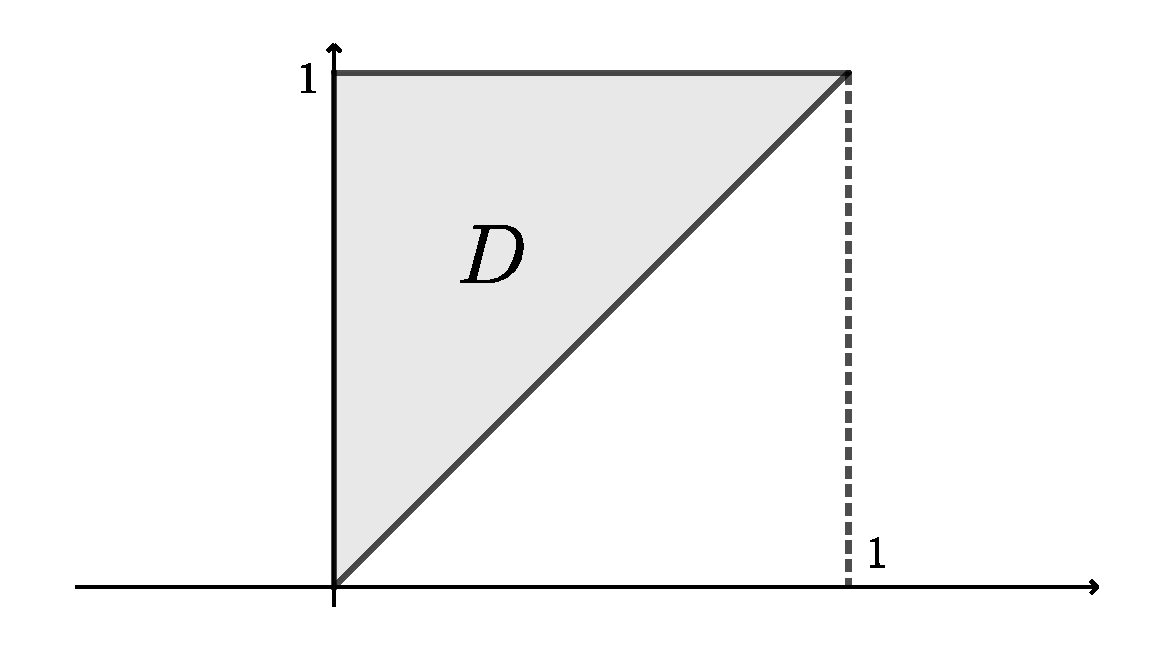
\includegraphics[height=4cm]{./pictures/no2.pdf}
       \caption{$D=\Set{ (x,y) \ | \ 0 \leq x \leq 1, \, x \leq y \leq 1 }$}\label{fig:no2}
     \end{figure}
     
     これより $D$ は横線集合として
     \[
       D= \Set{ (x,y)  |  0 \leq y \leq 1, \, 0 \leq x \leq y}
     \]
     と表せるので,重積分は以下の累次積分に書き直せる.
     \begin{align*}
       \iint_{D} \sin \left( \pi y^2\right) \ dy dx
       &= \int_{0}^{1} \left(\int_{0}^{y} \sin (\pi y^2) \ dx \right) dy
         = \int_{0}^{1} \Big[ x \sin (\pi y^2) \Big]_{x=0}^{x=y} \ dy\\
       &=\int_{0}^{1} y \sin (\pi y^2) \ dy = \left[-\frac{1}{2\pi}
         \cos (\pi y^2) \right]_{0}^{1}=\frac{1}{\pi}.
     \end{align*}
     
   \item 閉領域 $D$ を $xy$ 平面に図示すると,図\ref{fig:no3}の通りである.
     \begin{figure}[h]
       \centering
       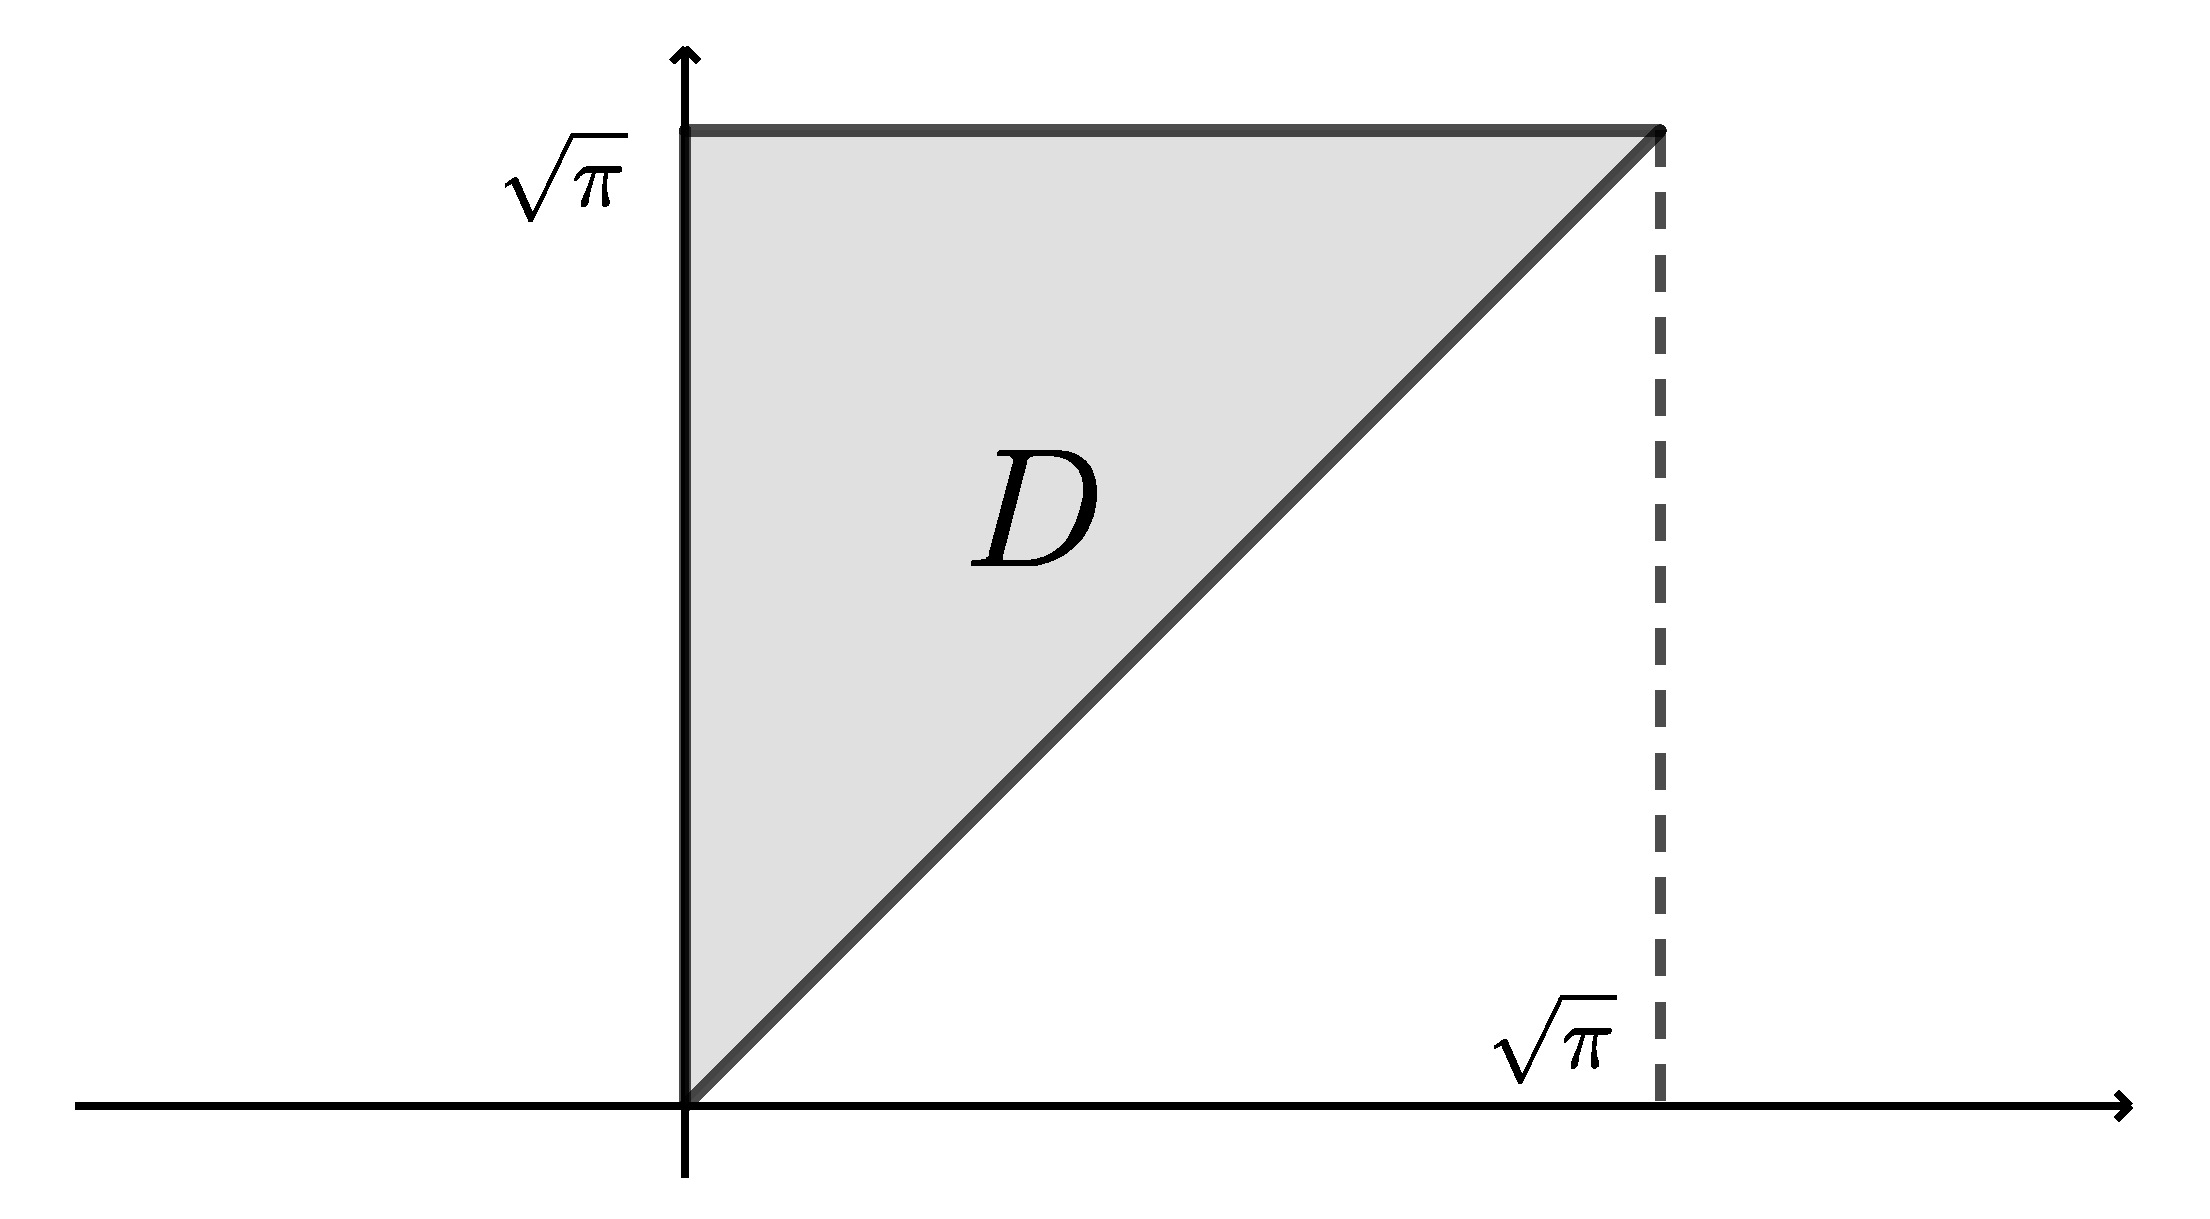
\includegraphics[height=4cm]{./pictures/no3.pdf}
       \caption{$D=\Set{ (x,y) \ | \ 0 \leq x \leq y, \, 0 \leq y \leq \sqrt{\pi} }$}\label{fig:no3}
     \end{figure}
     
     $D$ を横線集合と見なして重積分を累次積分に書き直せばよい.
     \begin{align*}
       \iint_{D} x^2 \cos (y^2) \ dx dy 
       &= \int_{0}^{\sqrt{\pi}} \left( \int_{0}^{y} x^2 \cos (y^2) \ dx \right)dy
         = \int_{0}^{\sqrt{\pi}} \left[ \frac{1}{3} x^3 \cos(y^2) \right]_{x=0}^{x=y} \ dy\\
       &= \frac{1}{3} \int_{0}^{\sqrt{\pi}} y^3 \cos (y^2) \ dy 
         = \frac{1}{3} \left[\frac{1}{2} y^2 \sin(y^2) + \frac{1}{2}\cos(y^2)\right]_{0}^{\sqrt{\pi}}\\
       &=-\frac{1}{3}.
     \end{align*}


   \item 閉領域 $D$ を $xy$ 平面に図示すると,図\ref{fig:no4}の通りである.
     \begin{figure}[h]
       \centering
       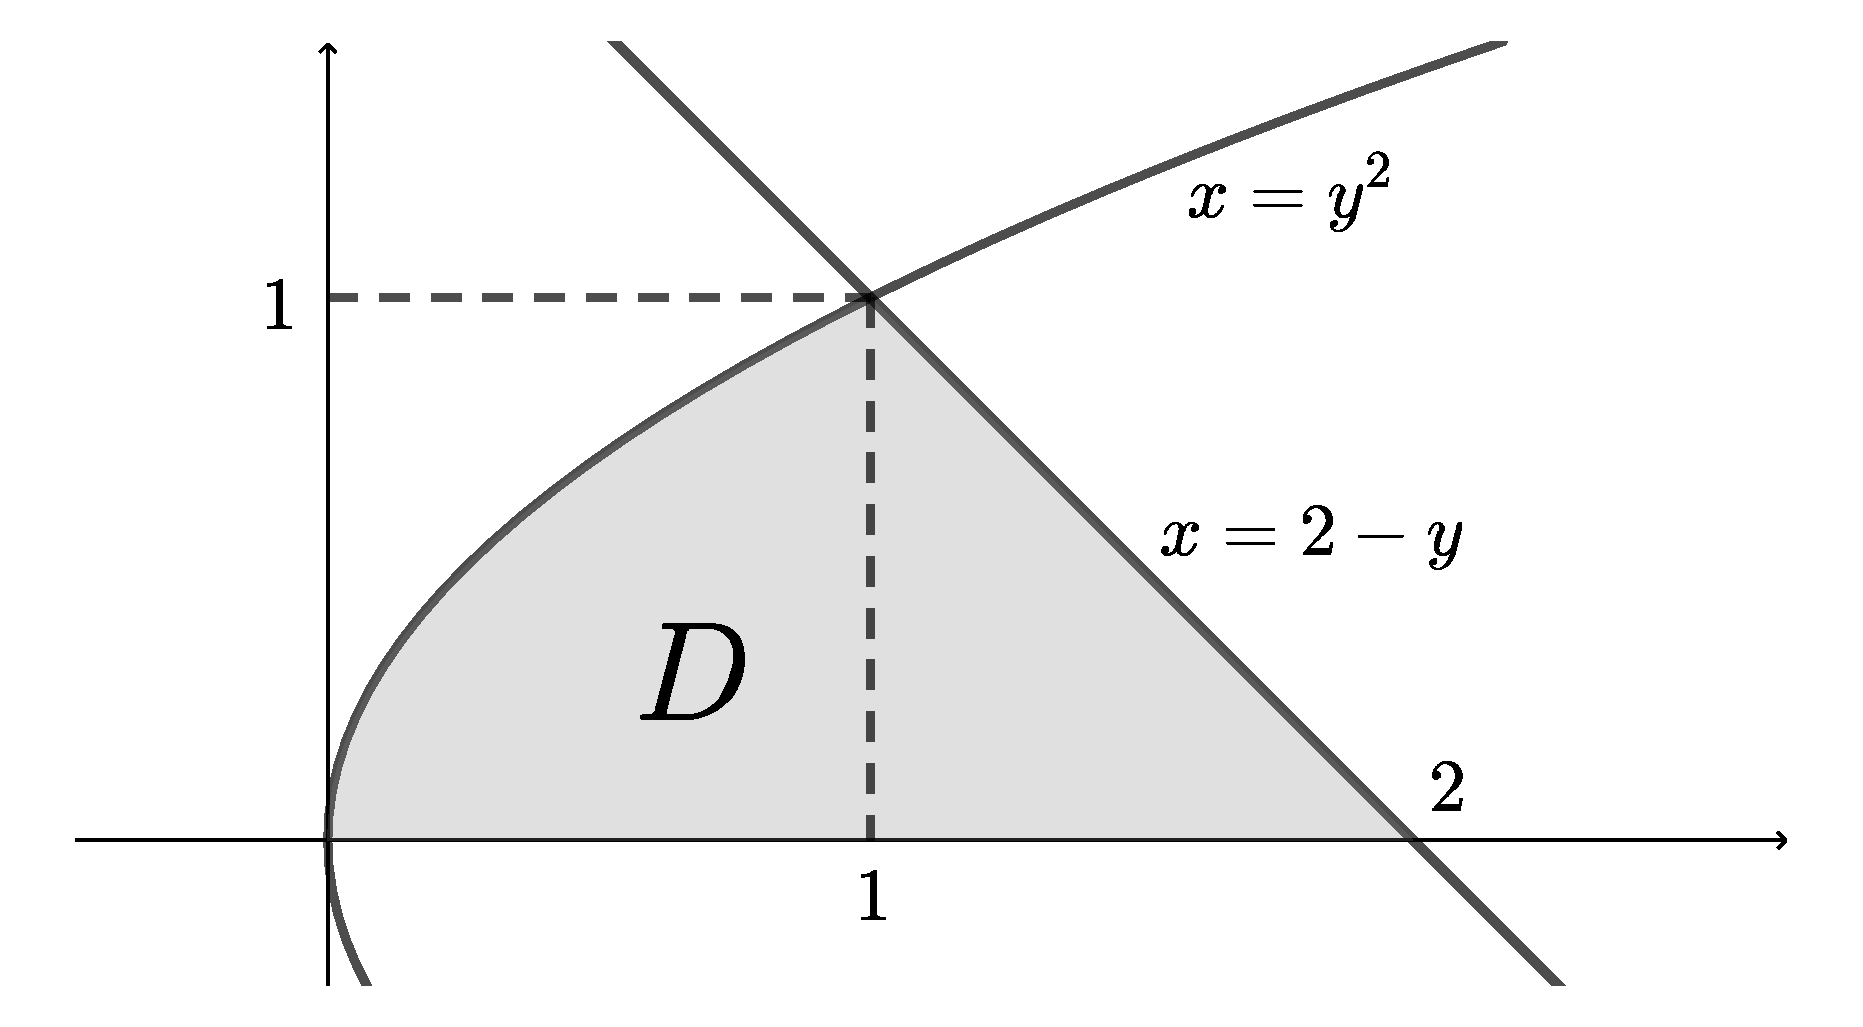
\includegraphics[height=4cm]{./pictures/no4.pdf}
       \caption{$D=\Set{(x,y) \ | \ x+y \leq 2, \, y^2 \leq x, \, 0 \leq y }$} \label{fig:no4}
     \end{figure}
     
     これより $D$ は横線集合として
     \[
       D=\Set{ (x,y)  |  0 \leq y \leq 1, \, y^2 \leq x \leq 2-y }
     \]
     と表せるので,重積分は以下の累次積分に書き直せる.
     \begin{align*}
       \iint_D xy \ dx dy 
       &= \int_{0}^{1} \left( \int_{y^2}^{2-y} xy \ dx \right) dy
         =\int_{0}^{1} \left[ \frac{1}{2}x^2y \right]_{x=y^2}^{x=2-y} \ dx\\
       &=\int_{0}^{1} \left( -\frac{1}{2}y^5 + \frac{1}{2} y^3 - 2y^2 + 2y \right) dy
         =\frac{3}{8}.
     \end{align*}
     
   \item 閉領域 $D$ を $xy$ 平面に図示すると,図\ref{fig:no5}の通りである.
    \begin{figure}[h]
       \centering
       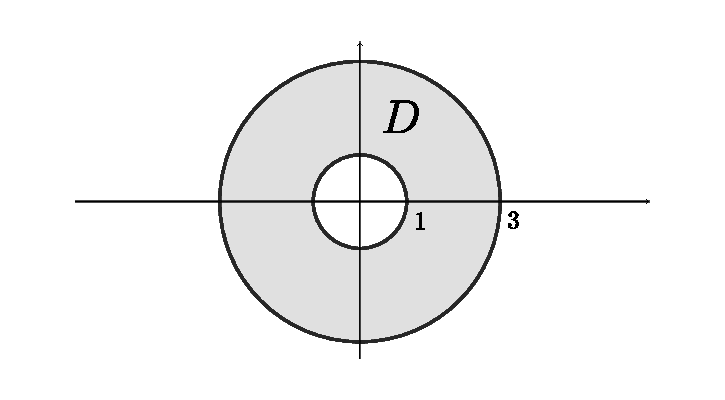
\includegraphics[height=3.5cm]{./pictures/no5.pdf}
       \caption{$D=\Set{ (x,y) \ | \ 1 \leq x^2+y^2 \leq 9}$}\label{fig:no5}        
     \end{figure}

     極座標変換
     \[
       x=r\cos \theta, \; y=r \sin \theta
     \]
     によって $r\theta$ 平面上の集合
     \[
       E=\Set{ (r, \theta)  |  1 \leq r \leq 3, \, 0 \leq \theta < 2\pi}
     \]
     が $xy$ 平面上の閉領域 $D$ に変換される.集合 $E$ を $r\theta$ 平面に図
     示すると図\ref{fig:no5p}の通りである.
     \begin{figure}[h]
       \centering
       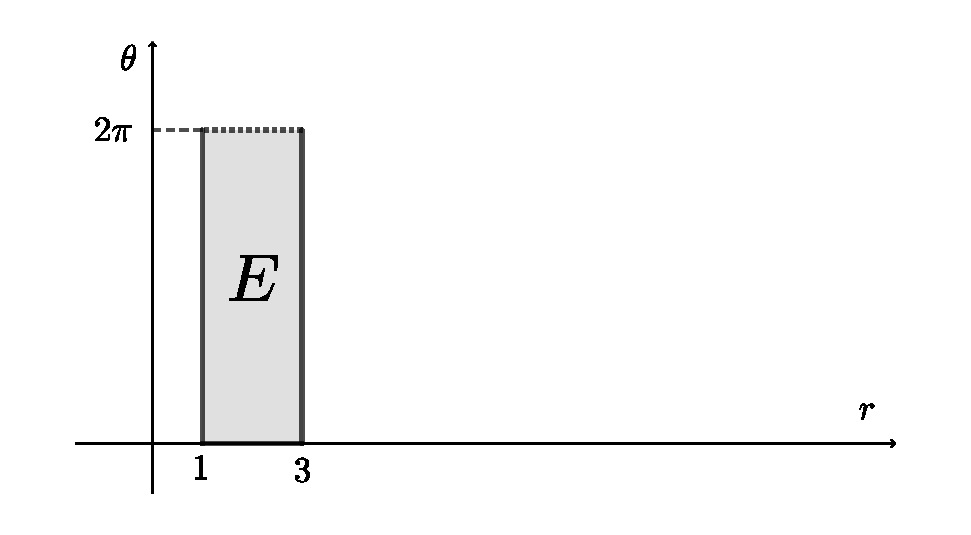
\includegraphics[height=4cm]{./pictures/no5p.pdf}
       \caption{$E=\Set{(r,\theta) \ | \ 1 \leq r \leq 3, \, 0 \leq \theta < 2 \pi}$}\label{fig:no5p}
     \end{figure}

     変換のヤコビアンは
     \begin{spacing}{1.3}    
       \[
         J(r, \theta) = \left|
           \begin{array}{cc}
             \frac{\partial x}{\partial r} & \frac{\partial x}{\partial \theta}\\
             \frac{\partial y}{\partial r} & \frac{\partial y}{\partial \theta}
           \end{array}
         \right| = \left|
           \begin{array}{rr}
             \cos \theta & -r\sin \theta\\
             \sin \theta & r\cos \theta
           \end{array}
         \right| = r
       \]
     \end{spacing}
     であるから,重積分は以下の様に書き直せる.
     \begin{align*}
       \iint_D \log (x^2+y^2) \ dxdy 
       &= \iint_E (\log r^2)|J(r,\theta)| \ dr d\theta 
         = \int_{0}^{2\pi} \left(  \int_{1}^{3} 2r \log r \ dr \right) d\theta\\
       &= \int_{0}^{2\pi} \left[ r^2 \log r - \frac{1}{2}r^2 \right]_{1}^{3} d\theta
         =\left(9\log 3 - 4\right) \int_{0}^{2\pi} d\theta\\
       &= -8\pi +18\pi \log 3.
     \end{align*}

   \item 閉領域 $D$ を $xy$ 平面に図示すると,図\ref{fig:no6}の通りである.
     \begin{figure}[h]
       \centering
       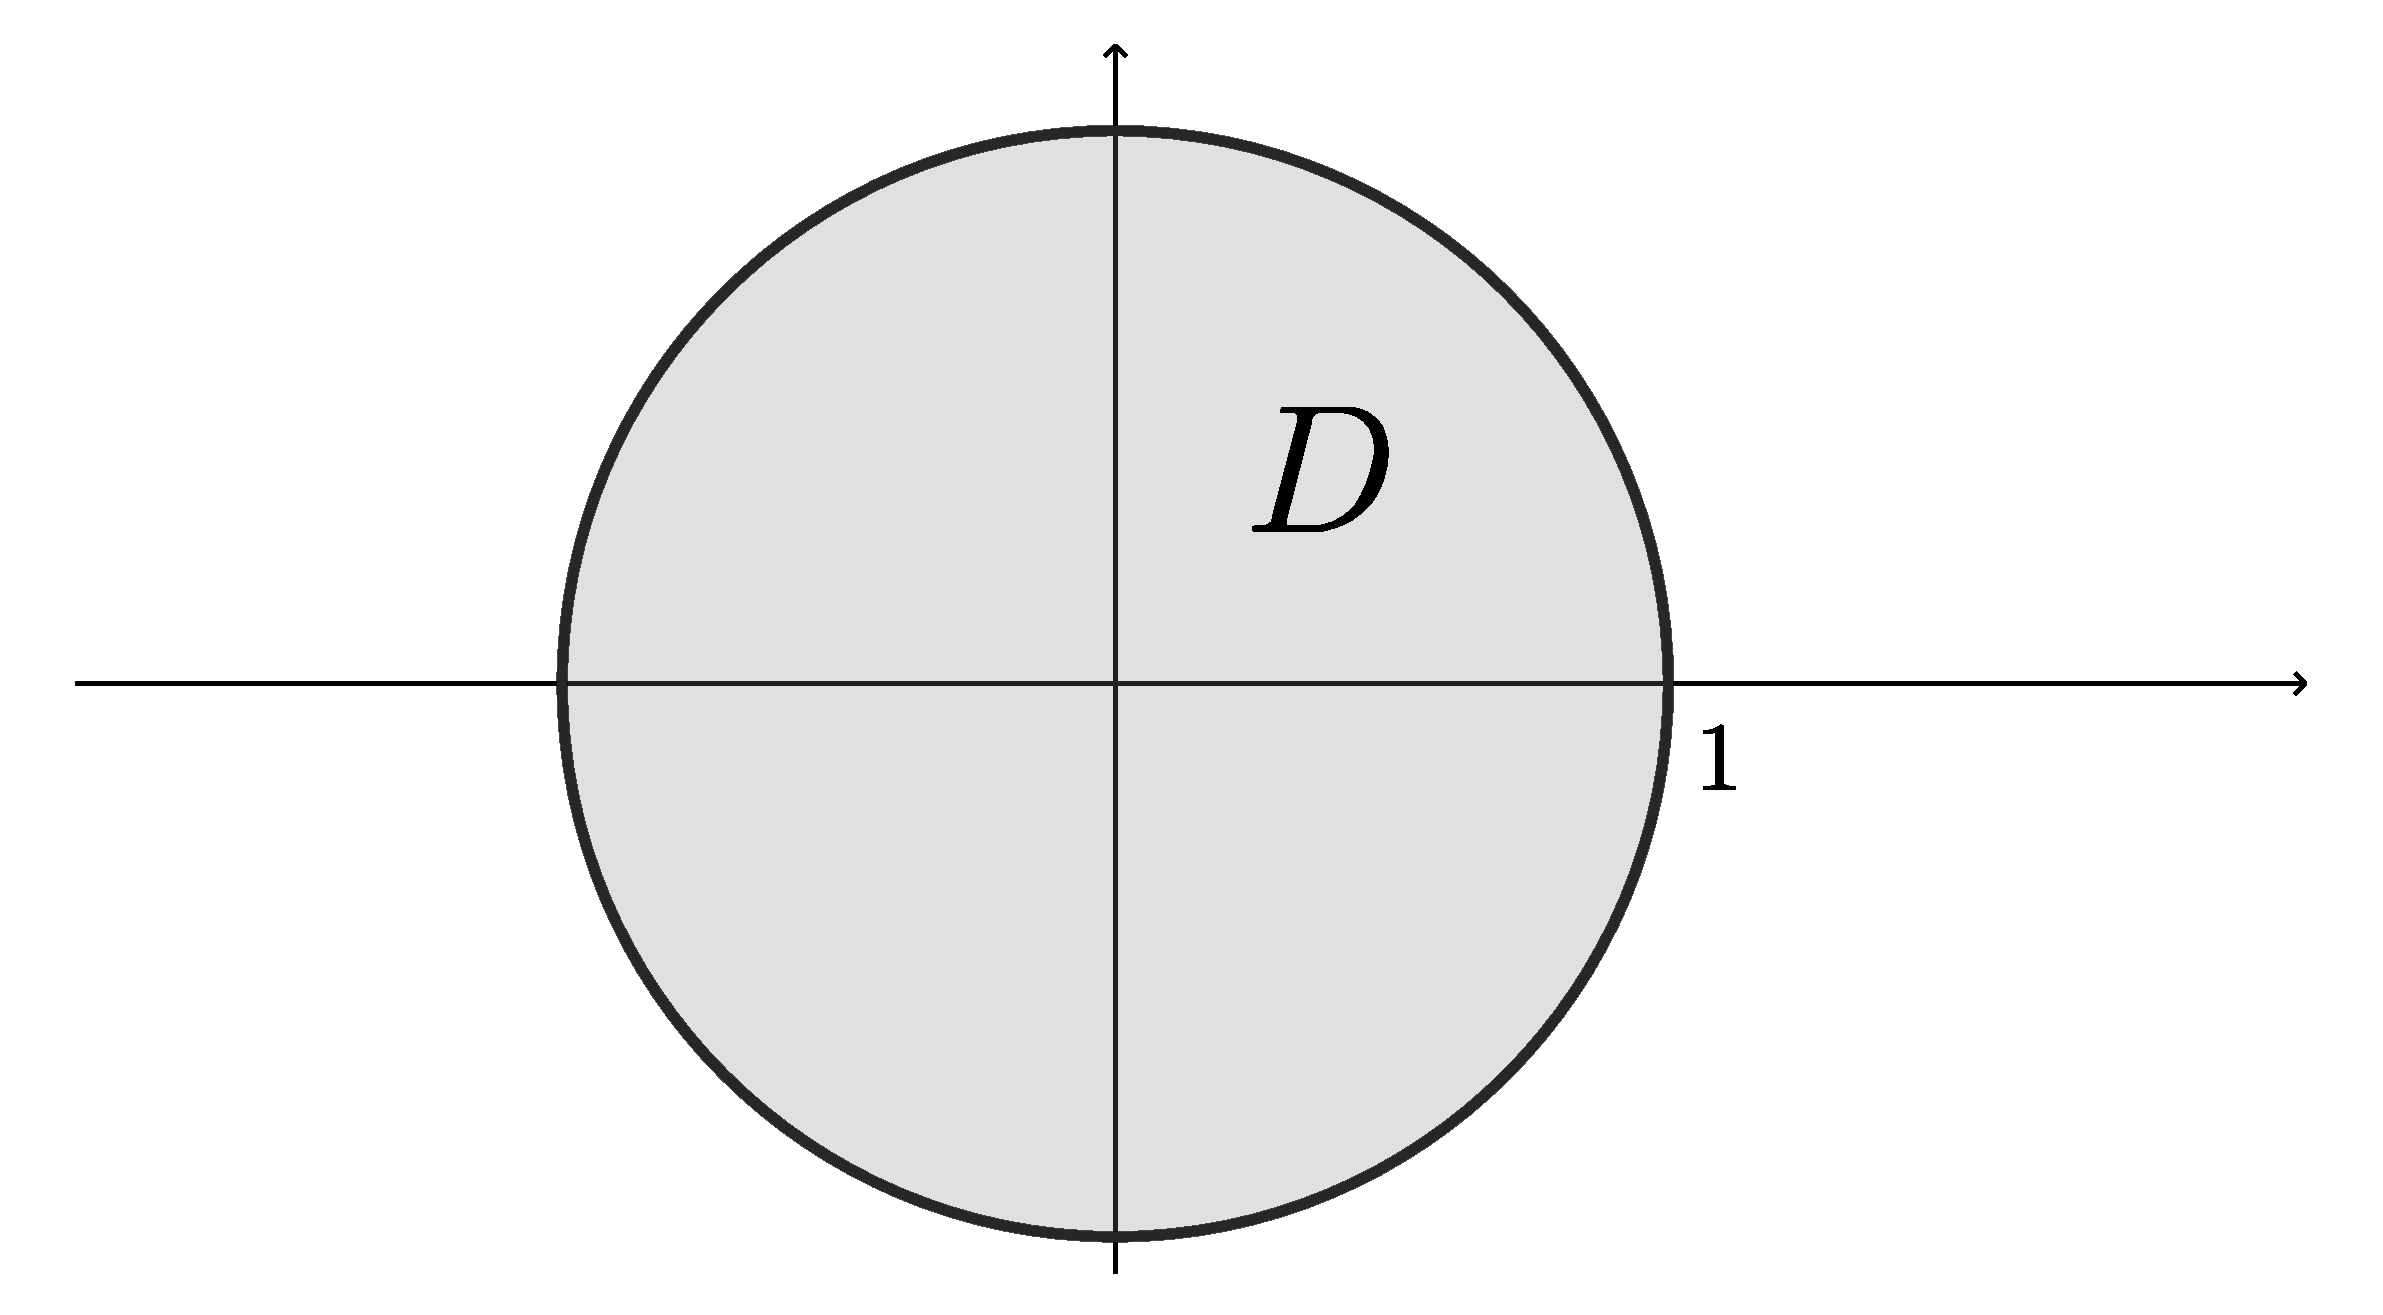
\includegraphics[height=3cm]{./pictures/no6.pdf}
       \caption{$D=\Set{ (x,y) \ | \  x^2+y^2 \leq 1}$}\label{fig:no6}        
     \end{figure}
     
     極座標変換
     \[
       x=r\cos \theta, \; y=r\sin \theta
     \]
     によって $r\theta$ 平面上の集合
     \[
       E=\Set{ (r, \theta)  |  0 \leq r \leq 1, \, 0 \leq \theta < 2\pi}
     \]
     が $xy$ 平面上の閉領域 $D$ に変換される.集合 $E$ を $r\theta$ 上に図示
     すると図\ref{fig:no6p}の通りである.
     \begin{figure}[h]     
       \centering
       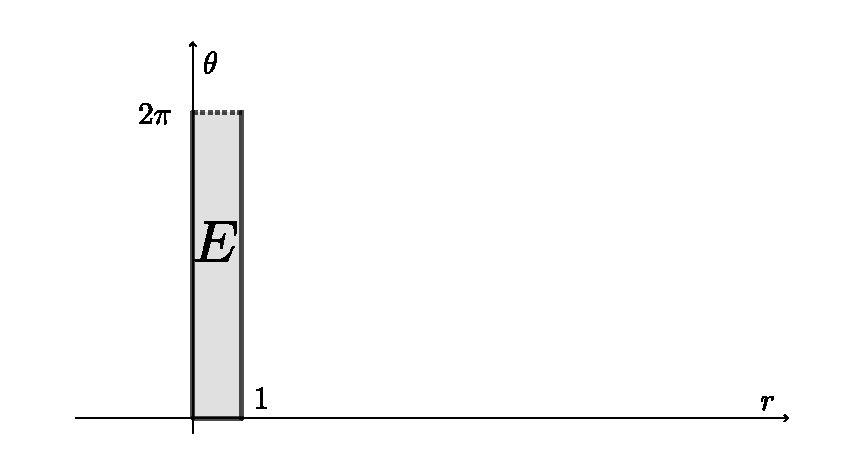
\includegraphics[height=4cm]{./pictures/no6p.pdf}
       \caption{$E=\Set{(r,\theta) \ | \ 0 \leq r \leq 1, \, 0 \leq \theta < 2 \pi}$}\label{fig:no6p}
     \end{figure}
   
     変換のヤコビアンは $J(r,\theta)=r$ であるから,重積分は以下の様に書き直せる.
     \begin{align*}
       \iint_D e^{-x^2-y^2} \ dx dy
       &= \iint_E -e^{r^2} |J(r,\theta)| \ dr d\theta 
         =\int_{0}^{2\pi} \left( \int_{0}^{1} r e^{-r^2} \ dr \right) d\theta\\
       & =\int_{0}^{2\pi} \left[-\frac{1}{2} e^{-r^2}\right]_{0}^{1} \ d\theta
       = \frac{1}{2} \left( 1-e^{-1} \right) \int_{0}^{2\pi} d\theta = \pi (1-e^{-1}).
     \end{align*}
            
   \item 閉領域 $D$ を $xy$ 平面に図示すると,図\ref{fig:no7}の通りである.
     \begin{figure}[h]
       \centering
       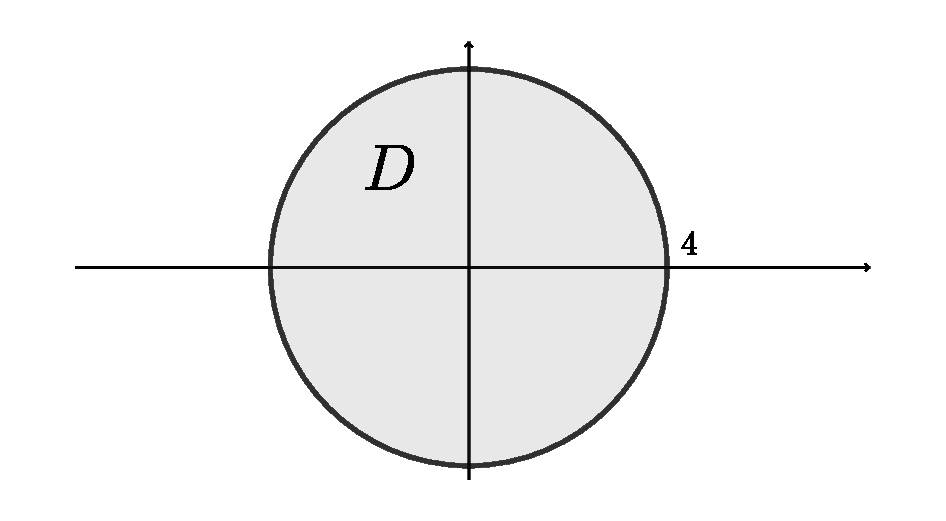
\includegraphics[height=4cm]{./pictures/no7.pdf}
       \caption{$D=\Set{ (x,y) \ | \  x^2+y^2 \leq 16}$}\label{fig:no7}        
     \end{figure}

     極座標変換
     \[
       x=r\cos\theta, \; y=r\sin\theta
     \]
     によって $r\theta$ 平面上の集合
     \[
       E=\Set{ (r, \theta)  |  0 \leq r \leq 4, \, 0 \leq \theta < 2\pi }
     \]
     が $xy$ 平面上の閉領域 $D$ に変換される.集合 $E$ を $r\theta$ 平面上に
     図示すると,図\ref{fig:no7p}の通りである.
     \begin{figure}[h]
       \centering
       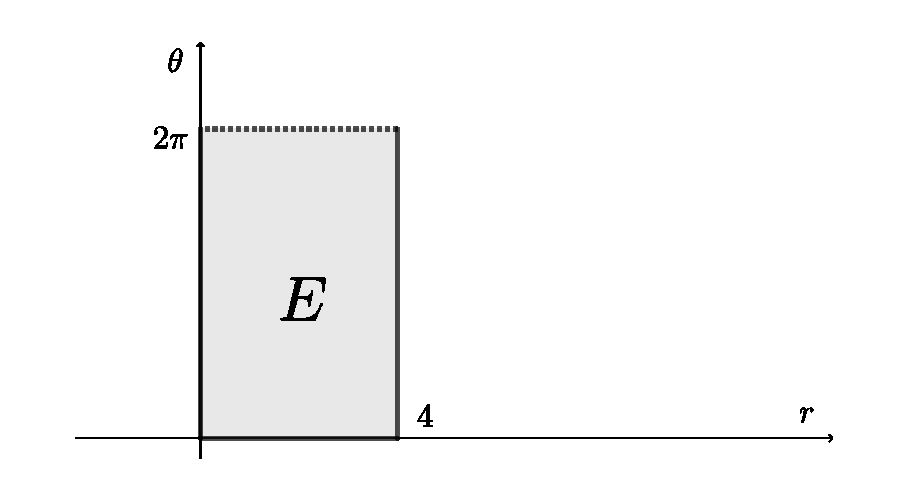
\includegraphics[height=4cm]{./pictures/no7p.pdf}
       \caption{$E=\Set{(r,\theta) \ | \ 0 \leq r \leq 4, \, 0 \leq \theta < 2 \pi}$}\label{fig:no7p}
     \end{figure}

     変換のヤコビアンは $J(r,\theta)=r$ であるから,重積分は以下の様に書き直せる.
     \begin{align*}
       \iint_D \cos (x^2+y^2) \ dx dy 
       &= \iint_E \cos(r^2) |J(r,\theta)| \ dr d\theta 
         = \int_{0}^{2\pi} \left( \int_{0}^{4} r\cos(r^2) \ dr \right) d\theta\\
       &= \int_{0}^{2\pi} \left[\frac{1}{2} \sin(r^2) \right]_{0}^{4} \ d\theta
         = \frac{1}{2} \sin 16\int_{0}^{2\pi} d\theta = \pi \sin 16.
     \end{align*}     

   \item 閉領域 $D$ を $xy$ 平面に図示すると,図\ref{fig:no8}の通りである.
     \begin{figure}[h]
       \centering
       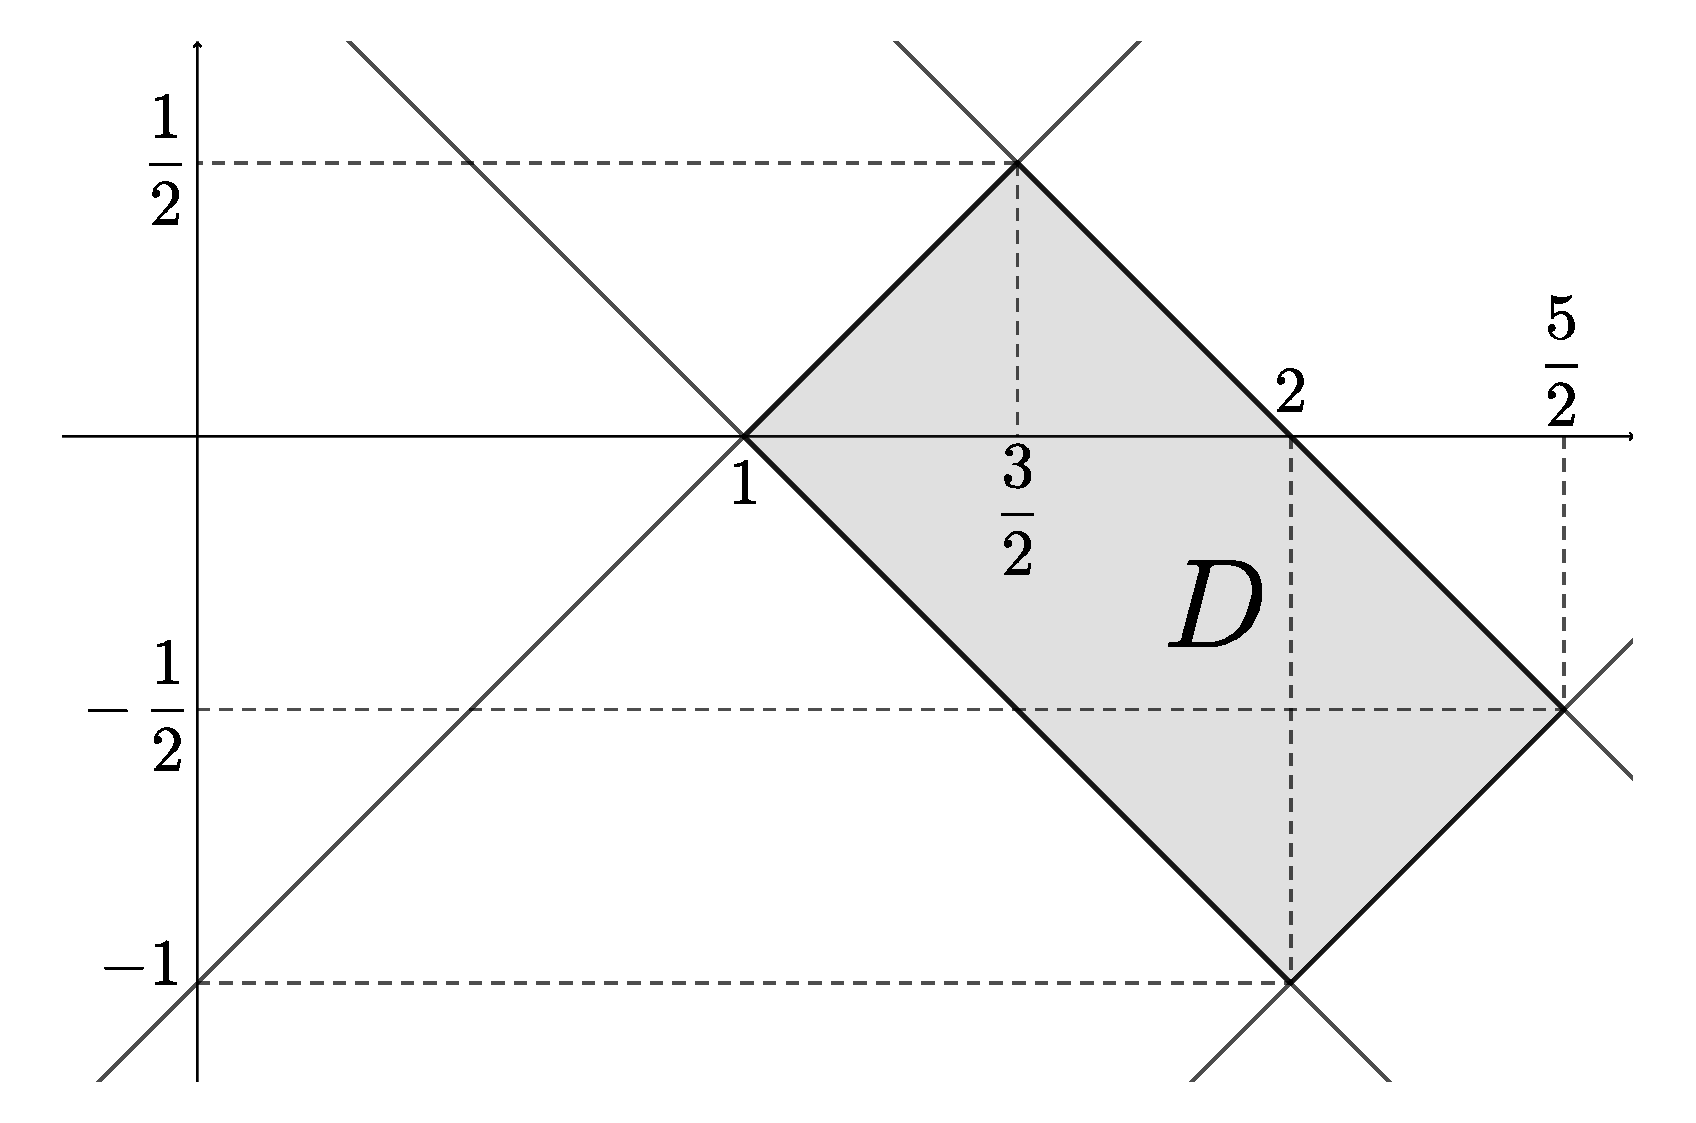
\includegraphics[height=4cm]{./pictures/no8.pdf}
       \caption{$D=\Set{ (x,y) \ | \  1 \leq x +y \leq 2, \, 1 \leq x-y \leq 3}$}\label{fig:no8}        
     \end{figure}

     変数変換
     \[
       u=x+y, \; v=x-y \; \left( \Leftrightarrow x= \frac{1}{2}u+\frac{1}{2}v, \, y=\frac{1}{2}u - \frac{1}{2}v \right)
     \]
     によって $uv$ 平面上の閉領域
     \[
       E=\Set{ (u,v)  |  1 \leq u \leq 3, \, 1 \leq v \leq 3}
     \]
     が $xy$ 平面上の閉領域 $D$ に変換される.閉領域 $E$ を $uv$ 平面に図示す
     ると,図\ref{fig:no8uv}の通りである.
     \begin{figure}[h]
       \centering
       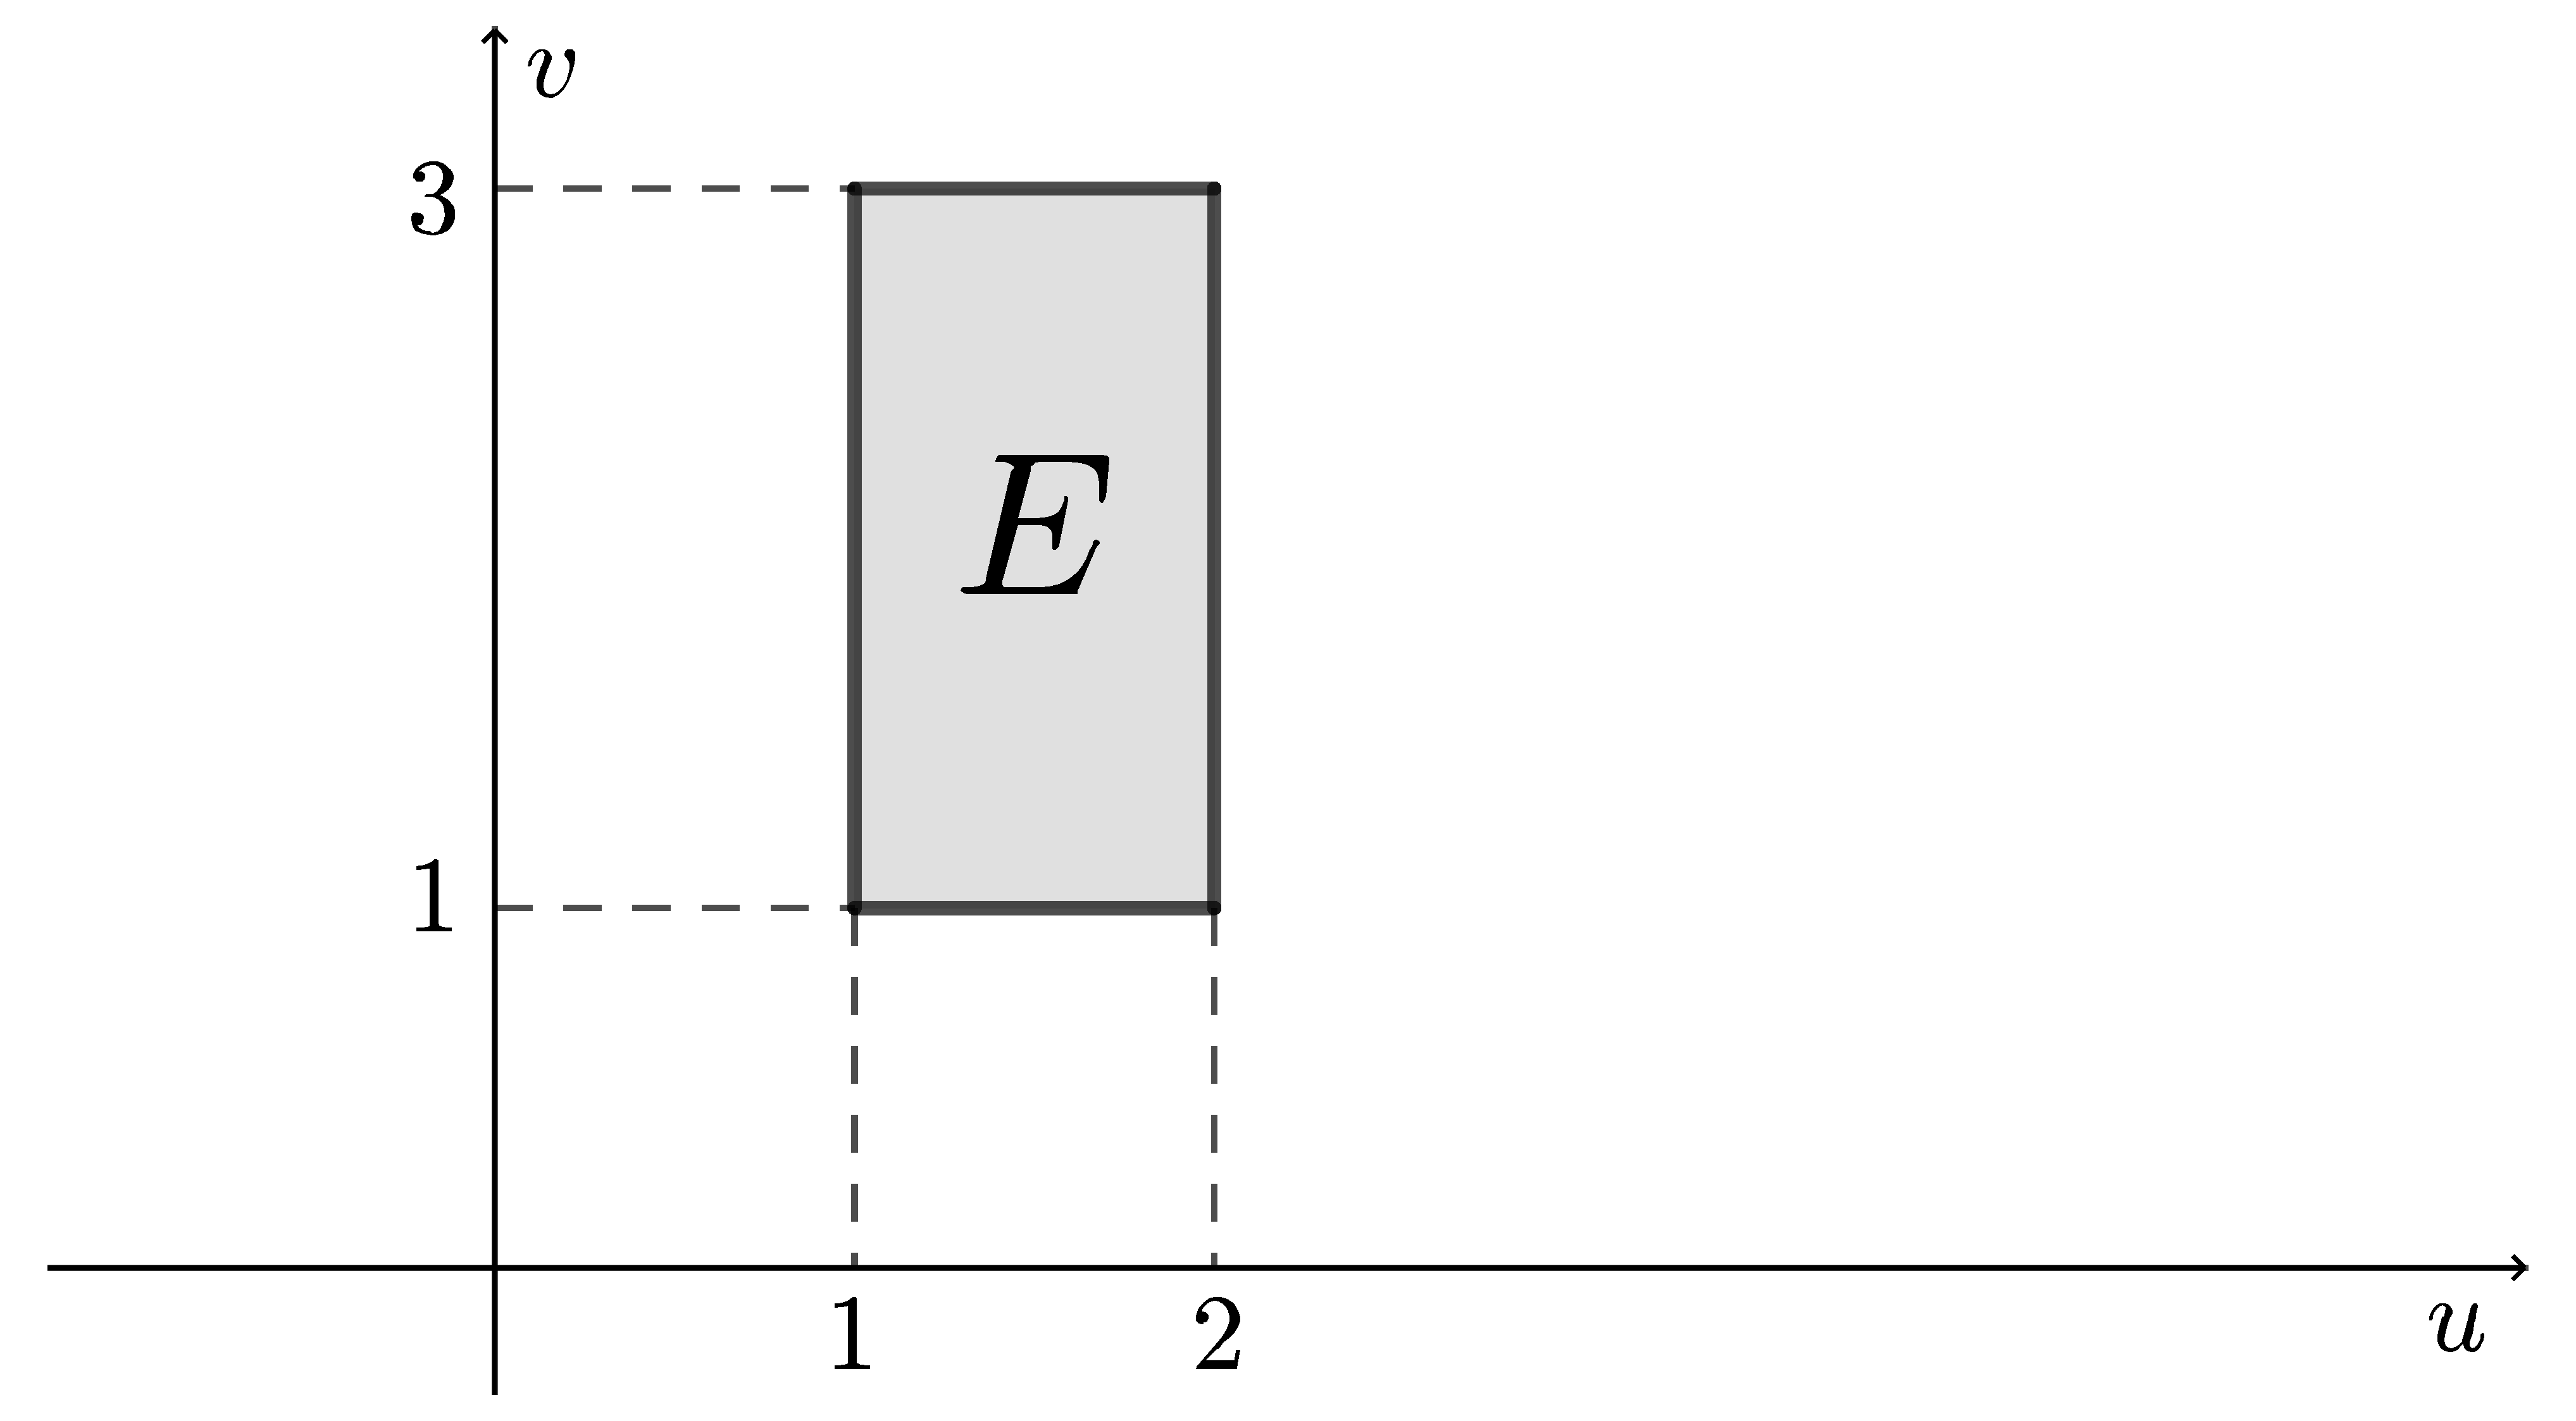
\includegraphics[height=4cm]{./pictures/no8uv.pdf}
       \caption{$E=\Set{(u,v) \ | \ 1 \leq u \leq 2, \, 1 \leq v \leq 3 }$}\label{fig:no8uv}
     \end{figure}
     
     変換のヤコビアンは
     \begin{spacing}{1.3}
       \[
         J(u, v) = \left|
           \begin{array}{cc}
             \frac{\partial x}{\partial u} & \frac{\partial x}{\partial v}\\
             \frac{\partial y}{\partial u} & \frac{\partial y}{\partial v}
           \end{array}
         \right| = \left|
           \begin{array}{rr}
             \frac{1}{2} & \frac{1}{2}\\
             \frac{1}{2} & -\frac{1}{2}
           \end{array}
         \right| = -\frac{1}{2}
       \]
     \end{spacing}
     であるから,重積分は以下の様に書き直せる.
     \begin{align*}
       \iint_D (x^2-y^2) \ dx dy 
       &= \iint_E uv |J(u,v)| \ du dv =\frac{1}{2} \int_{1}^{3}\left( \int_{1}^{2} uv \ du \right)dv\\
       &=\frac{1}{2} \int_1^3 \left[ \frac{1}{2} u^2 v \right]_{u=1}^{u=2} \ dv 
         =\frac{1}{4} \int_{1}^{3} 3v \ dv = 3.
     \end{align*}
     
   \item 閉領域 $D$ を $xy$ 平面に図示すると,図\ref{fig:no9}の通りである.
     \begin{figure}[h]
       \centering
       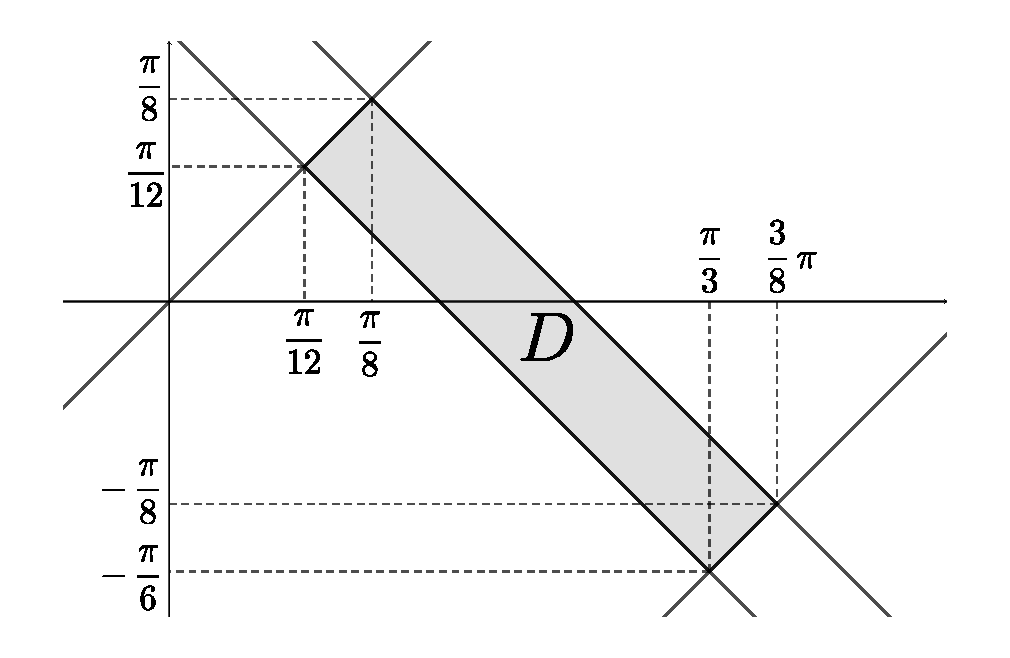
\includegraphics[height=4cm]{./pictures/no9.pdf}
       \caption{$D=\Set{ (x,y) | \frac{\pi}{6} \leq x +y \leq \frac{\pi}{4}, 
           0 \leq x-y \leq \frac{\pi}{2} }$}\label{fig:no9}          
     \end{figure}

     変数変換
     \[
       u=x+y, \, v=x-y \; \left( \Leftrightarrow x=\frac{u+v}{2}, \, y=\frac{u-v}{2} \right)
     \]
     によって $uv$ 平面上の閉領域
     \[
       E=\Set{ (u,v)  |  \frac{\pi}{6} \leq u \leq \frac{\pi}{4}, \, 0 \leq v \leq \frac{\pi}{2} }
     \]
     が $xy$ 平面上の閉領域 $D$ に変換される.閉領域 $E$ を $uv$ 平面に図示す
     ると,図\ref{fig:no9uv}の通りである.
     \begin{figure}[h]
       \centering
       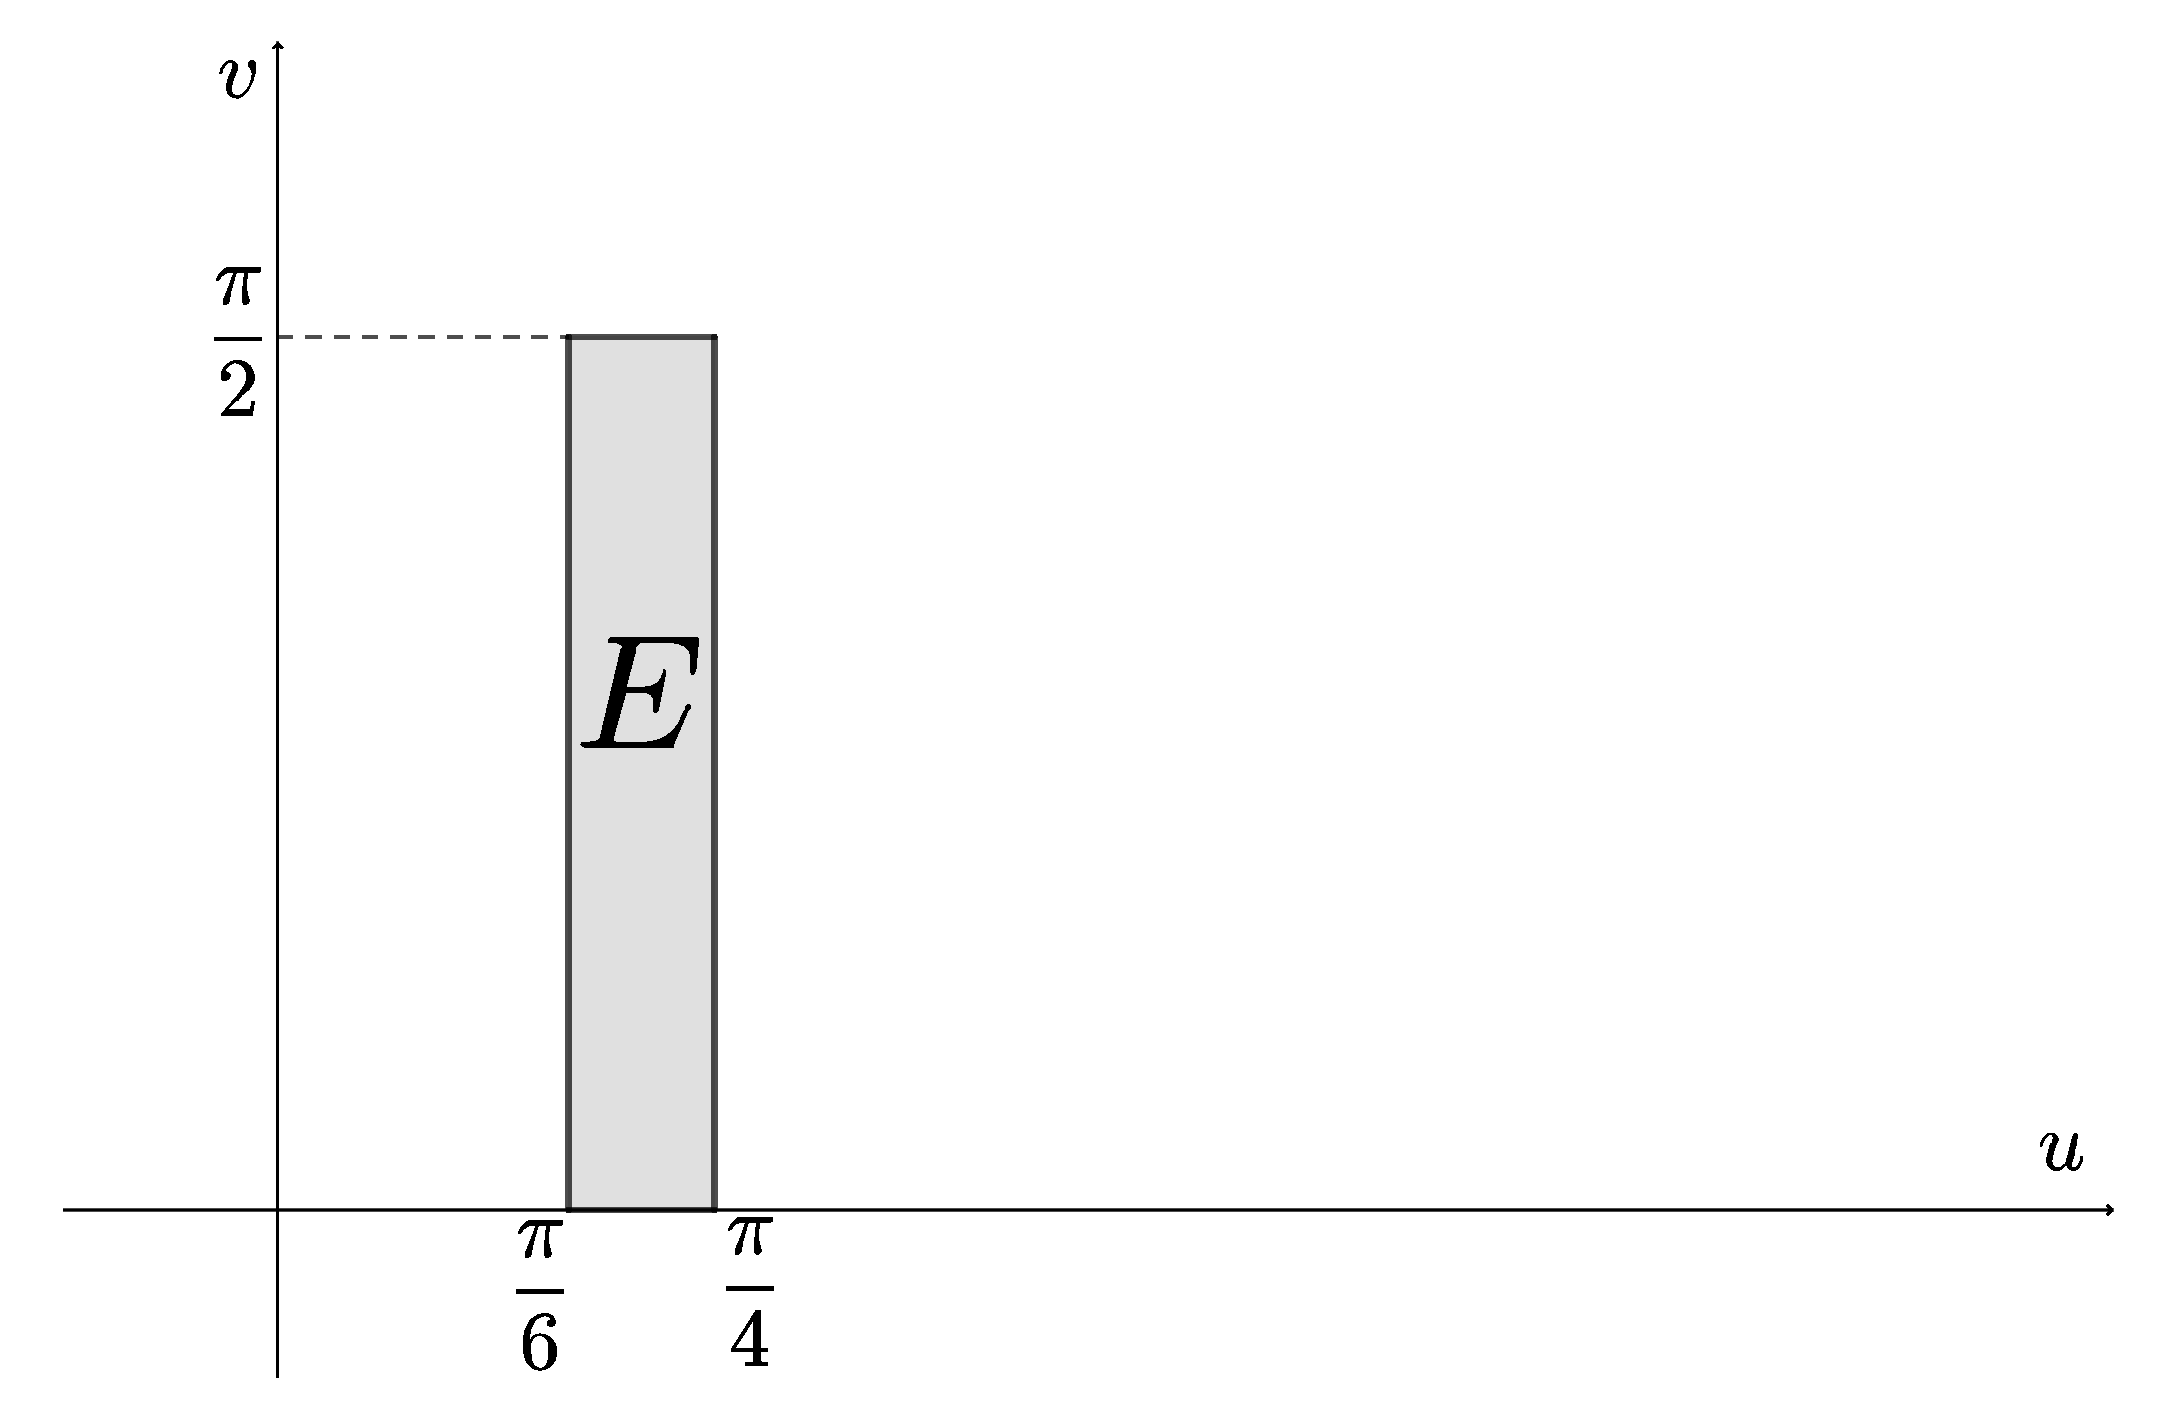
\includegraphics[height=4cm]{./pictures/no9uv.pdf}
       \caption{$E=\Set{(u,v) | \frac{\pi}{6} \leq u \leq \frac{\pi}{4}, 
           0 \leq v \leq \frac{\pi}{4} }$}\label{fig:no9uv}
     \end{figure}
 
     変換のヤコビアンは $J(u,v)=-\frac{1}{2}$ であるから,重積分は以下のように書き直せる.
     \begin{align*}
         \iint_D (x-y)\tan(x+y) \ dx dy 
       &= \iint_E v \tan u \ |J(u,v)| du dv
         = \frac{1}{2}\int_{0}^{\frac{\pi}{2}} 
         \left( \int_{\frac{\pi}{6}}^{\frac{\pi}{4}} v \tan u \ du \right) dv\\
       &= \frac{1}{2} \int_{0}^{\frac{\pi}{2}} v\Big[ -\log | \cos u |
         \Big]_{\frac{\pi}{6}}^{\frac{\pi}{4}} \ dv = \frac{1}{4}\log
         \frac{3}{2} \int_{0}^{\frac{\pi}{2}} v \ dv = \frac{\pi^2}{32}\log \frac{3}{2}.
     \end{align*}


   \item 閉領域 $D$ を $xy$ 平面上に図示すると,図\ref{fig:no10}の通りである.
     \begin{figure}[h]
       \centering
       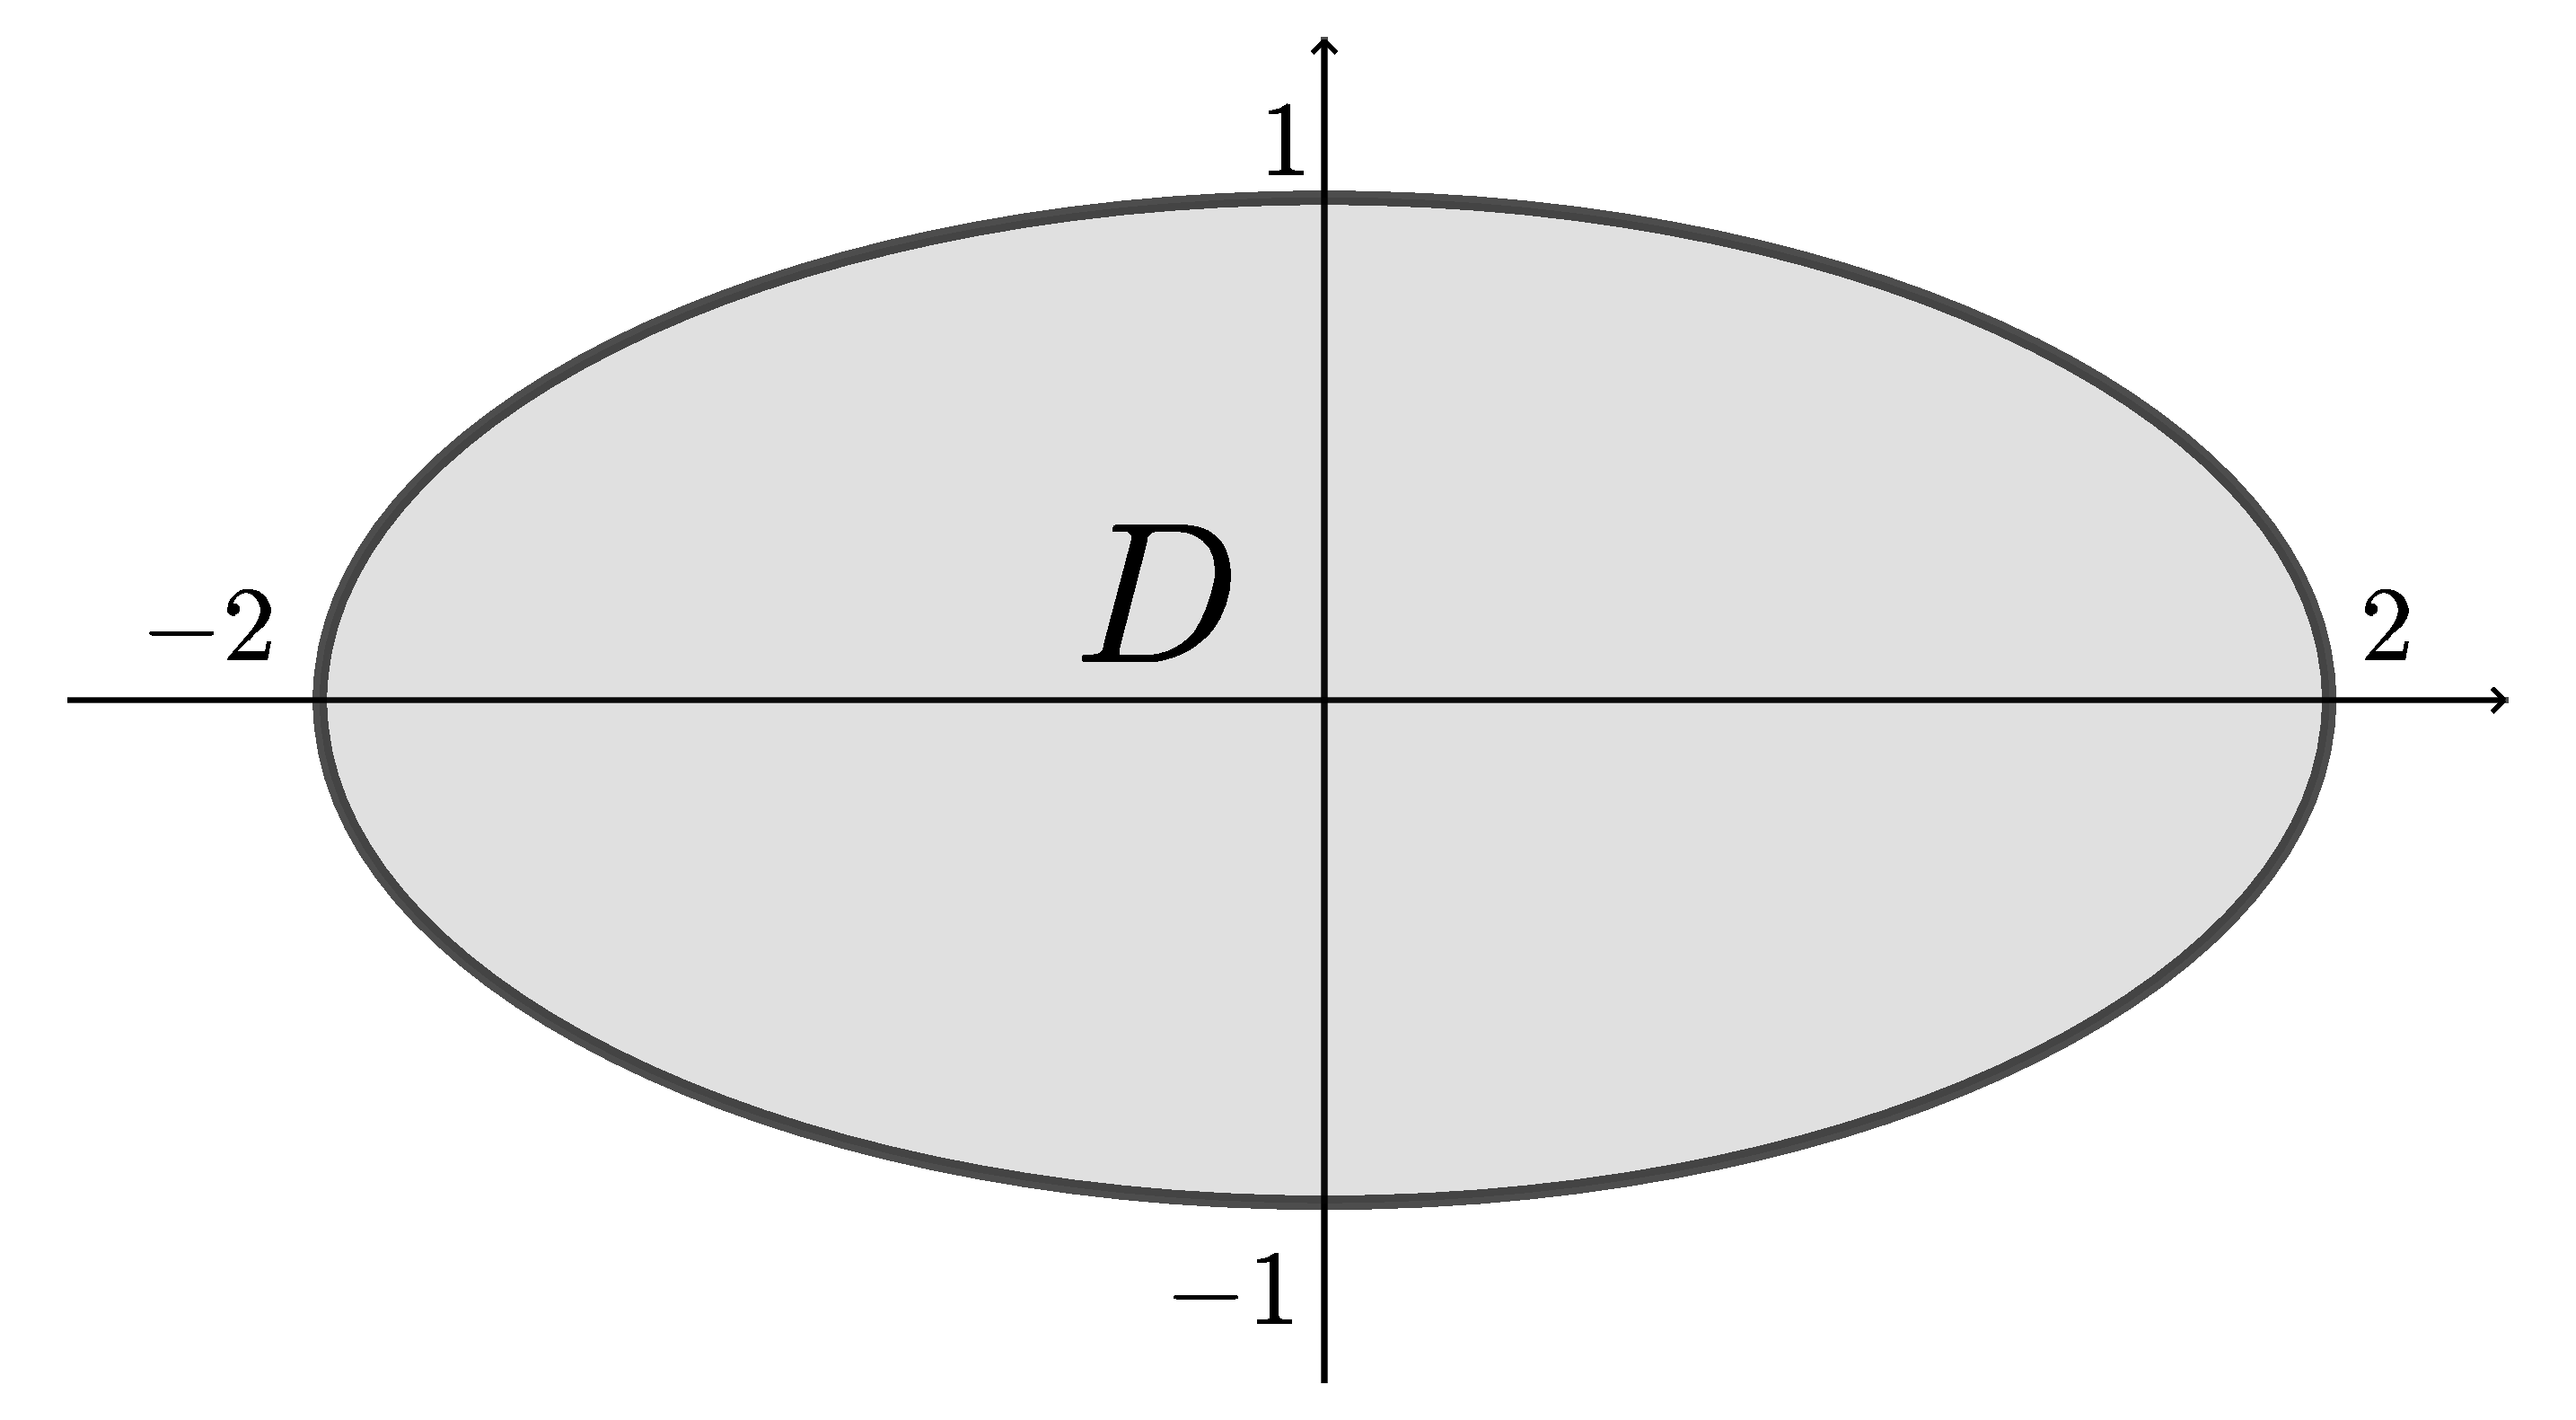
\includegraphics[height=4cm]{./pictures/no10.pdf}
       \caption{$D=\Set{ (x,y)  |  \frac{x^2}{4} + y^2 \leq 1}$}\label{fig:no10}              
     \end{figure}

     変数変換
     \[
       x=2r\cos \theta, \, y=r\sin \theta
     \]
     によって $r \theta$ 平面上の集合
     \[
       E=\Set{ (r, \theta) | 0 \leq r \leq 1, 0 \leq \theta < 2\pi }
     \]
     が $xy$ 平面上の閉領域 $D$ に変換される.集合 $E$ を $r\theta$ 平面上に
     図示すると,図\ref{fig:no10p}の通りである.
     \begin{figure}[h]
       \centering
       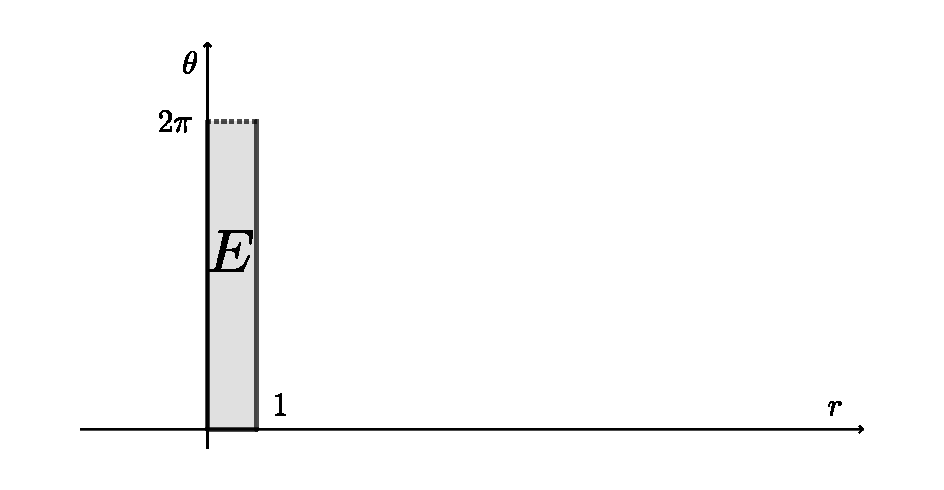
\includegraphics[height=4cm]{./pictures/no10p.pdf}
       \caption{$E=\Set{(u,v) | 0 \leq r \leq 1, \, 0 \leq \theta < 2\pi }$}\label{fig:no10p}       
     \end{figure}

     変換のヤコビアンは
     \begin{spacing}{1.3}
       \[
         J(r,\theta) = \left|
           \begin{array}{cc}
             \frac{\partial x}{\partial r} & \frac{\partial x}{\partial \theta}\\
             \frac{\partial y}{\partial r} & \frac{\partial y}{\partial \theta}
           \end{array}
         \right| = \left|
           \begin{array}{rr}
             2 \cos \theta & -2 r \sin \theta\\
             \sin \theta & r \cos \theta
           \end{array}
         \right| = 2r
       \]
     \end{spacing}
     であるから,重積分は以下の様に書き直せる.
       \begin{align*}
         \iint_D (x^2+y^2) \ dx dy &= \iint_E r^2(4\cos^2 \theta + \sin^2 \theta) |J(r,\theta)| \ dr d\theta\\
         &= 2 \int_{0}^{2\pi} \left( \int_{0}^{1} r^3 (3 \cos^2 \theta +1) \ dr \right) d\theta\\
         &= 2 \int_{0}^{2\pi} (3 \cos^2 \theta+1) \left[\frac{1}{4}r^4\right]_{0}^{1} d\theta\\
         &= \frac{1}{2} \int_{0}^{2\pi} (3\cos^2 \theta +1) \ d\theta = \frac{5}{2}\pi.
       \end{align*}

   \item 閉領域 $D$ を $xy$ 平面上に図示すると,図\ref{fig:no11}の通りである.
     \begin{figure}[h]
       \centering
       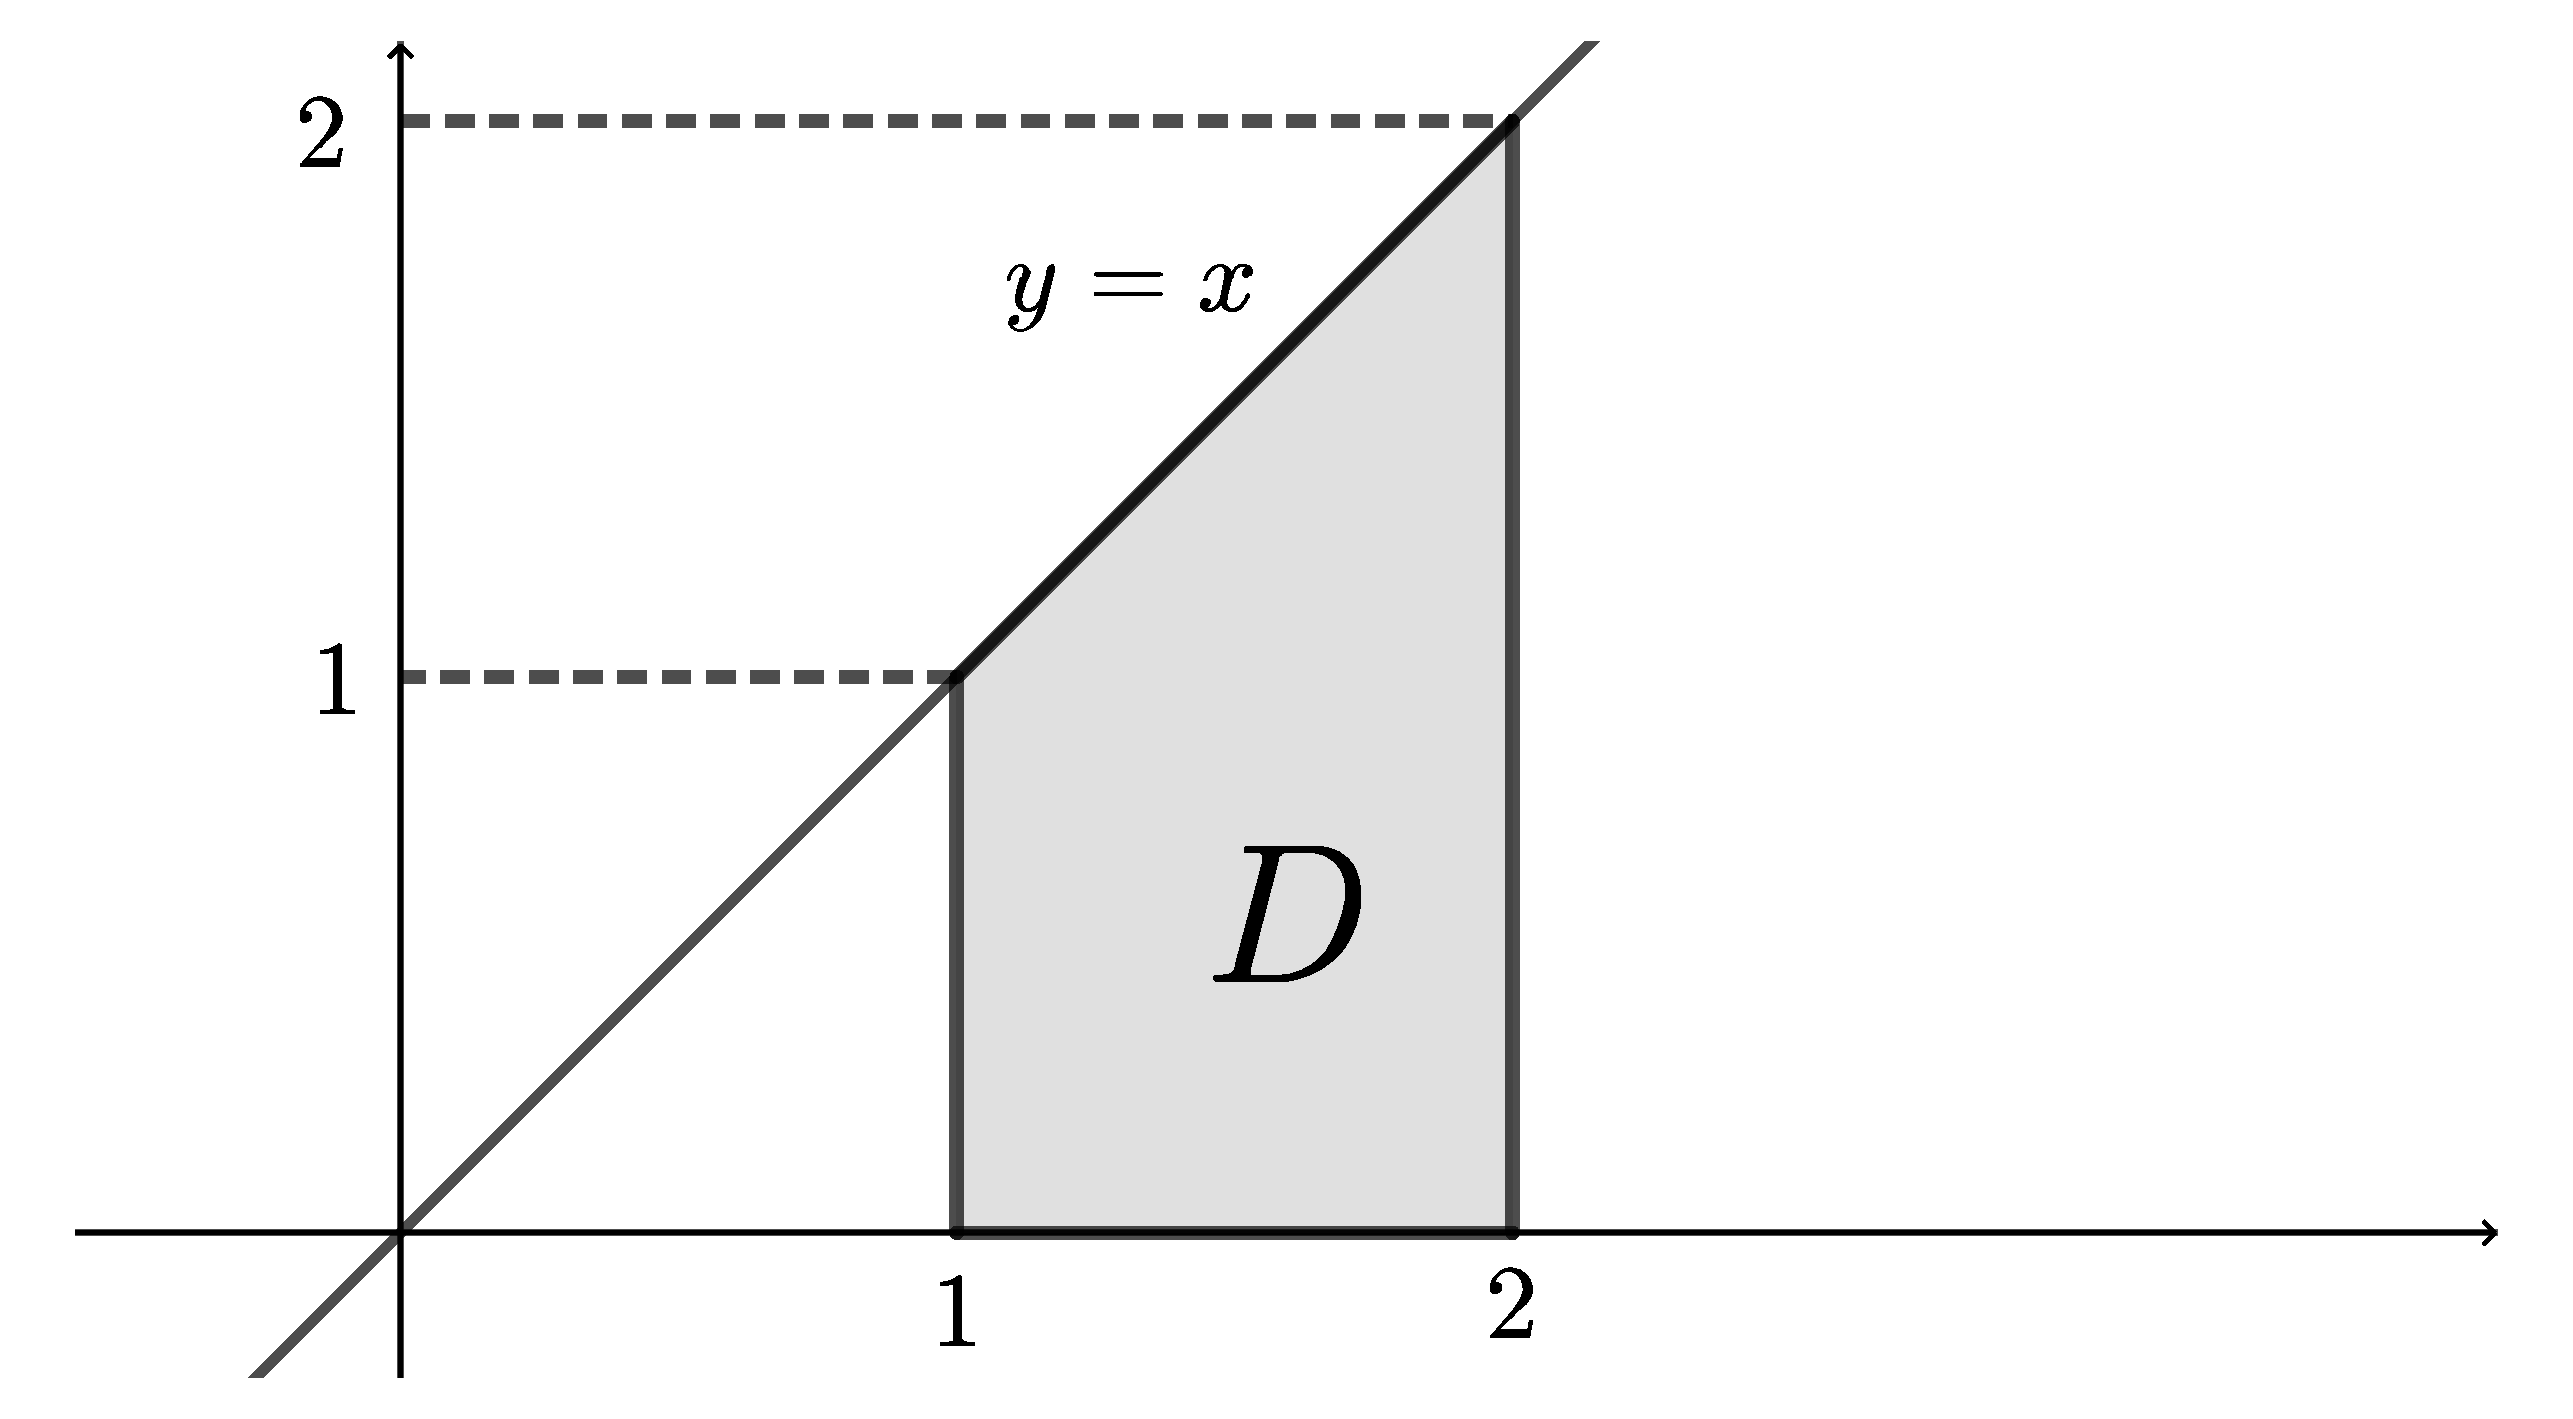
\includegraphics[height=4cm]{./pictures/no11.pdf}
       \caption{$D=\Set{ (x,y)  |  1 \leq x \leq 2, \, 0 \leq y \leq x }$}\label{fig:no11}        
     \end{figure}

     $D$ を縦線集合と見なして重積分を累次積分に書き直せばよい.
     \begin{align*}
       \iint_D \frac{xy}{x^2+y^2} \ dx dy 
       &= \int_{1}^{2} \left( \int_{0}^{x} \frac{xy}{x^2+y^2} \ dy \right) dx
         = \int_{1}^{2} \frac{x}{2}\left[\log(x^2+y^2)\right]_{y=0}^{y=x} \ dx\\
       &= \frac{\log 2}{2} \int_{1}^{2}  x \ dx = \frac{3}{4} \log 2.
     \end{align*}
     
   \item 閉領域 $D$ を $xy$ 平面に図示すると図\ref{fig:no12}の通りである.
     \begin{figure}[h]
       \centering
       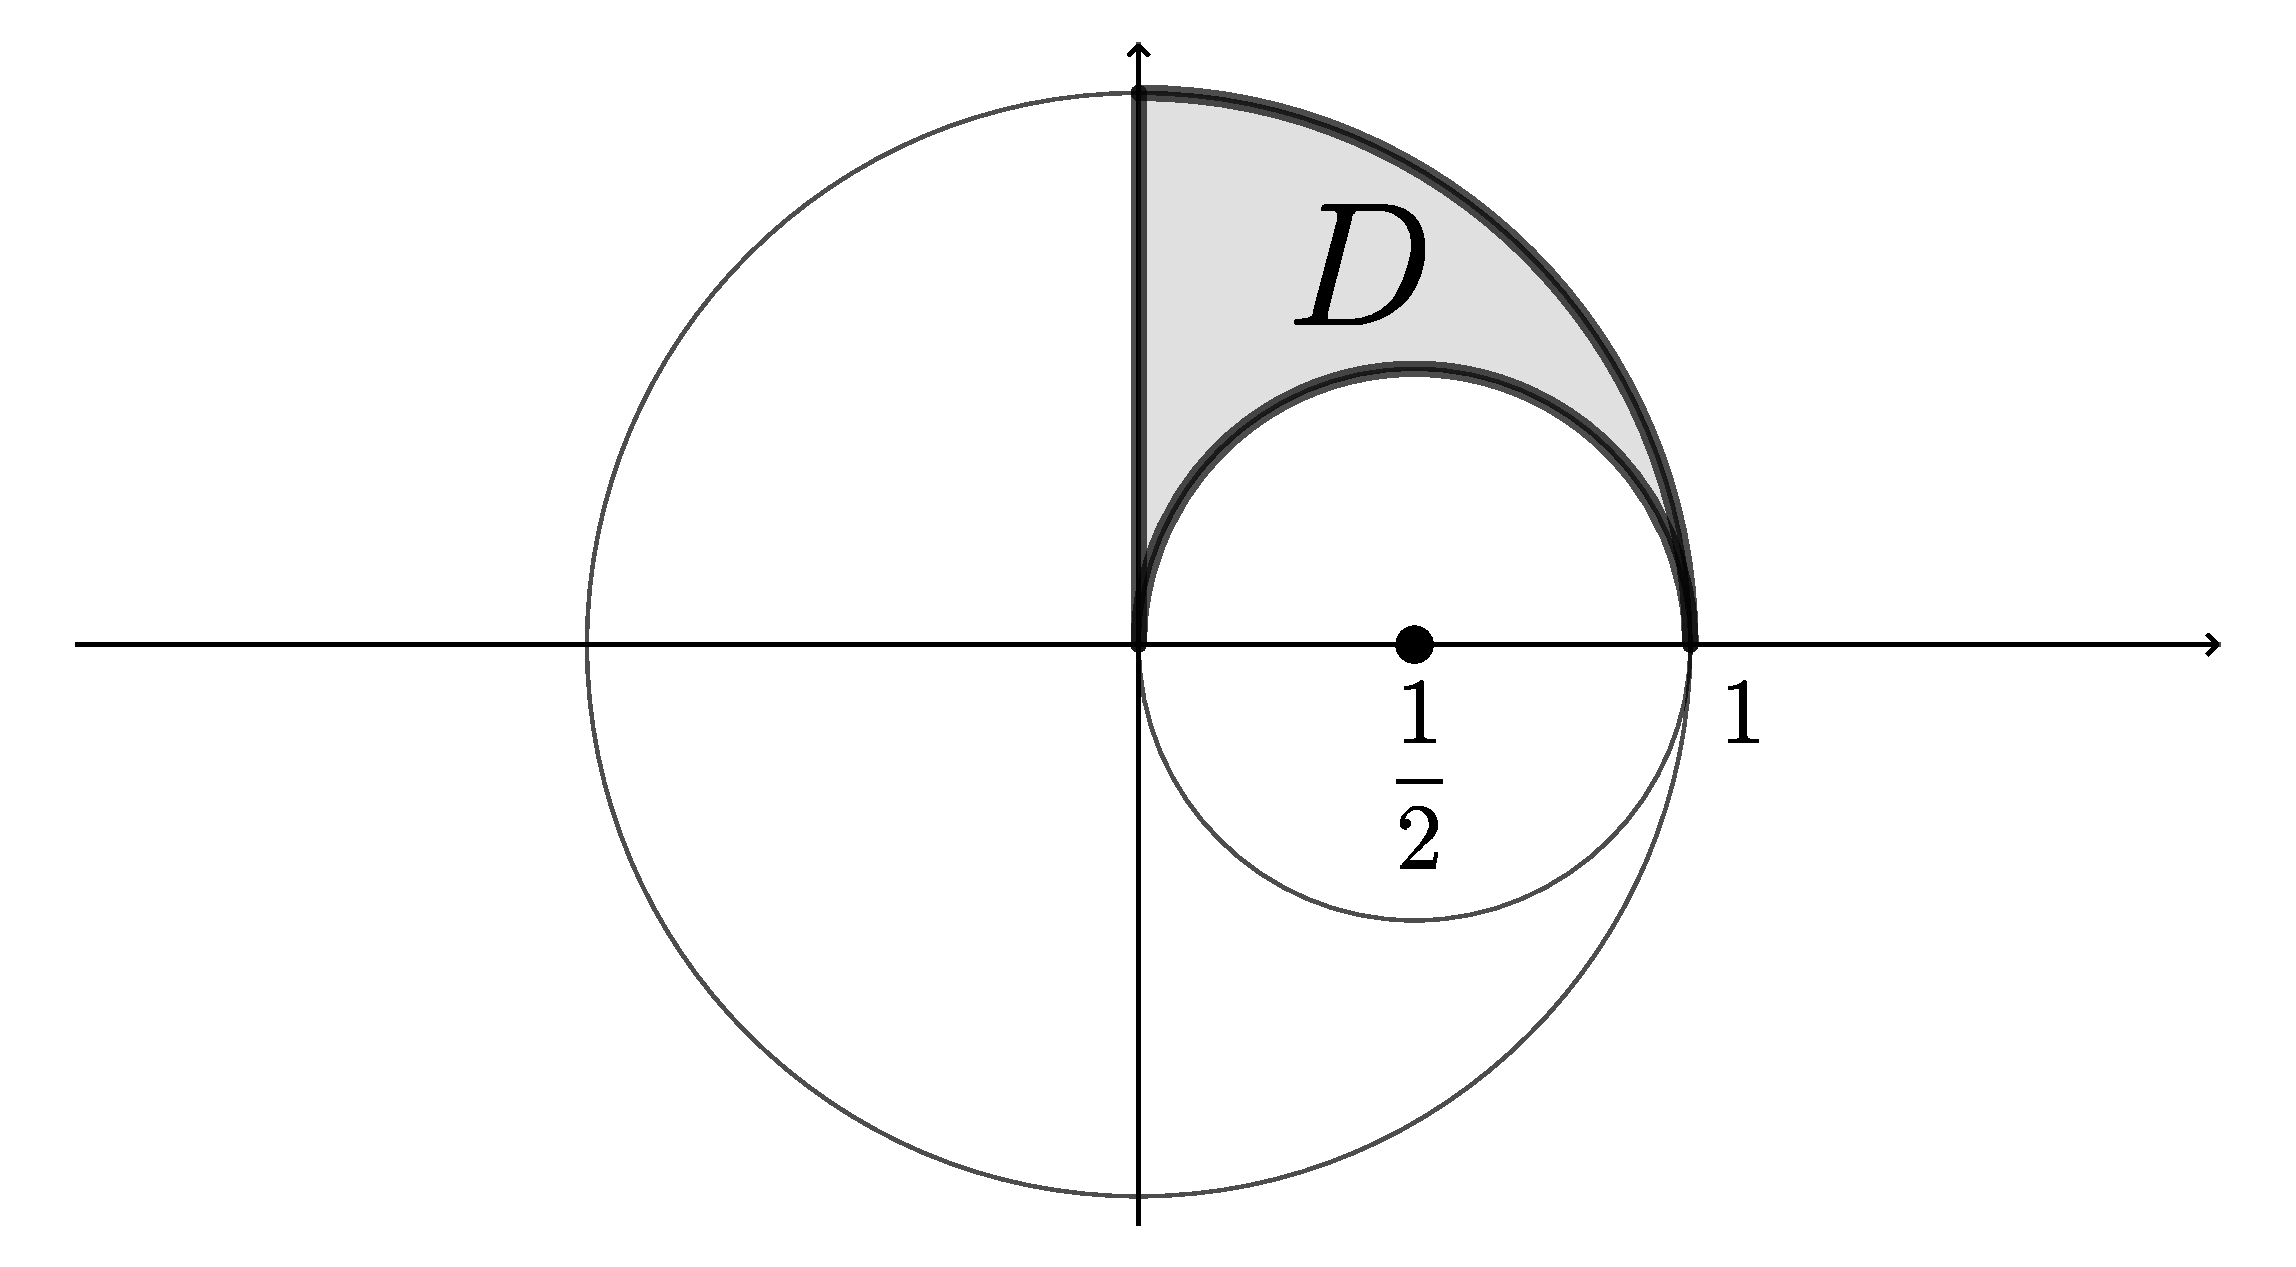
\includegraphics[height=4cm]{./pictures/no12.pdf}
       \caption{$D=\Set{ (x,y) | 0 \leq x \leq x^2+y^2 \leq 1, 0 \leq y }$}\label{fig:no12}       
     \end{figure}

     極座標変換
     \[
       x=r\cos\theta, \; y=r\sin\theta
     \]
     によって $r\theta$ 平面上の閉領域
     \[
       E=\Set{ (r, \theta)  |  0 \leq \theta \leq \frac{\pi}{2}, \, \cos\theta \leq r \leq 1}
     \]
     が $xy$ 平面上の閉領域 $D$ に変換される.閉領域 $E$ を $r\theta$ 平
     面に図示すると,図\ref{fig:no12p}の通りである.
     \begin{figure}[h]
       \centering
       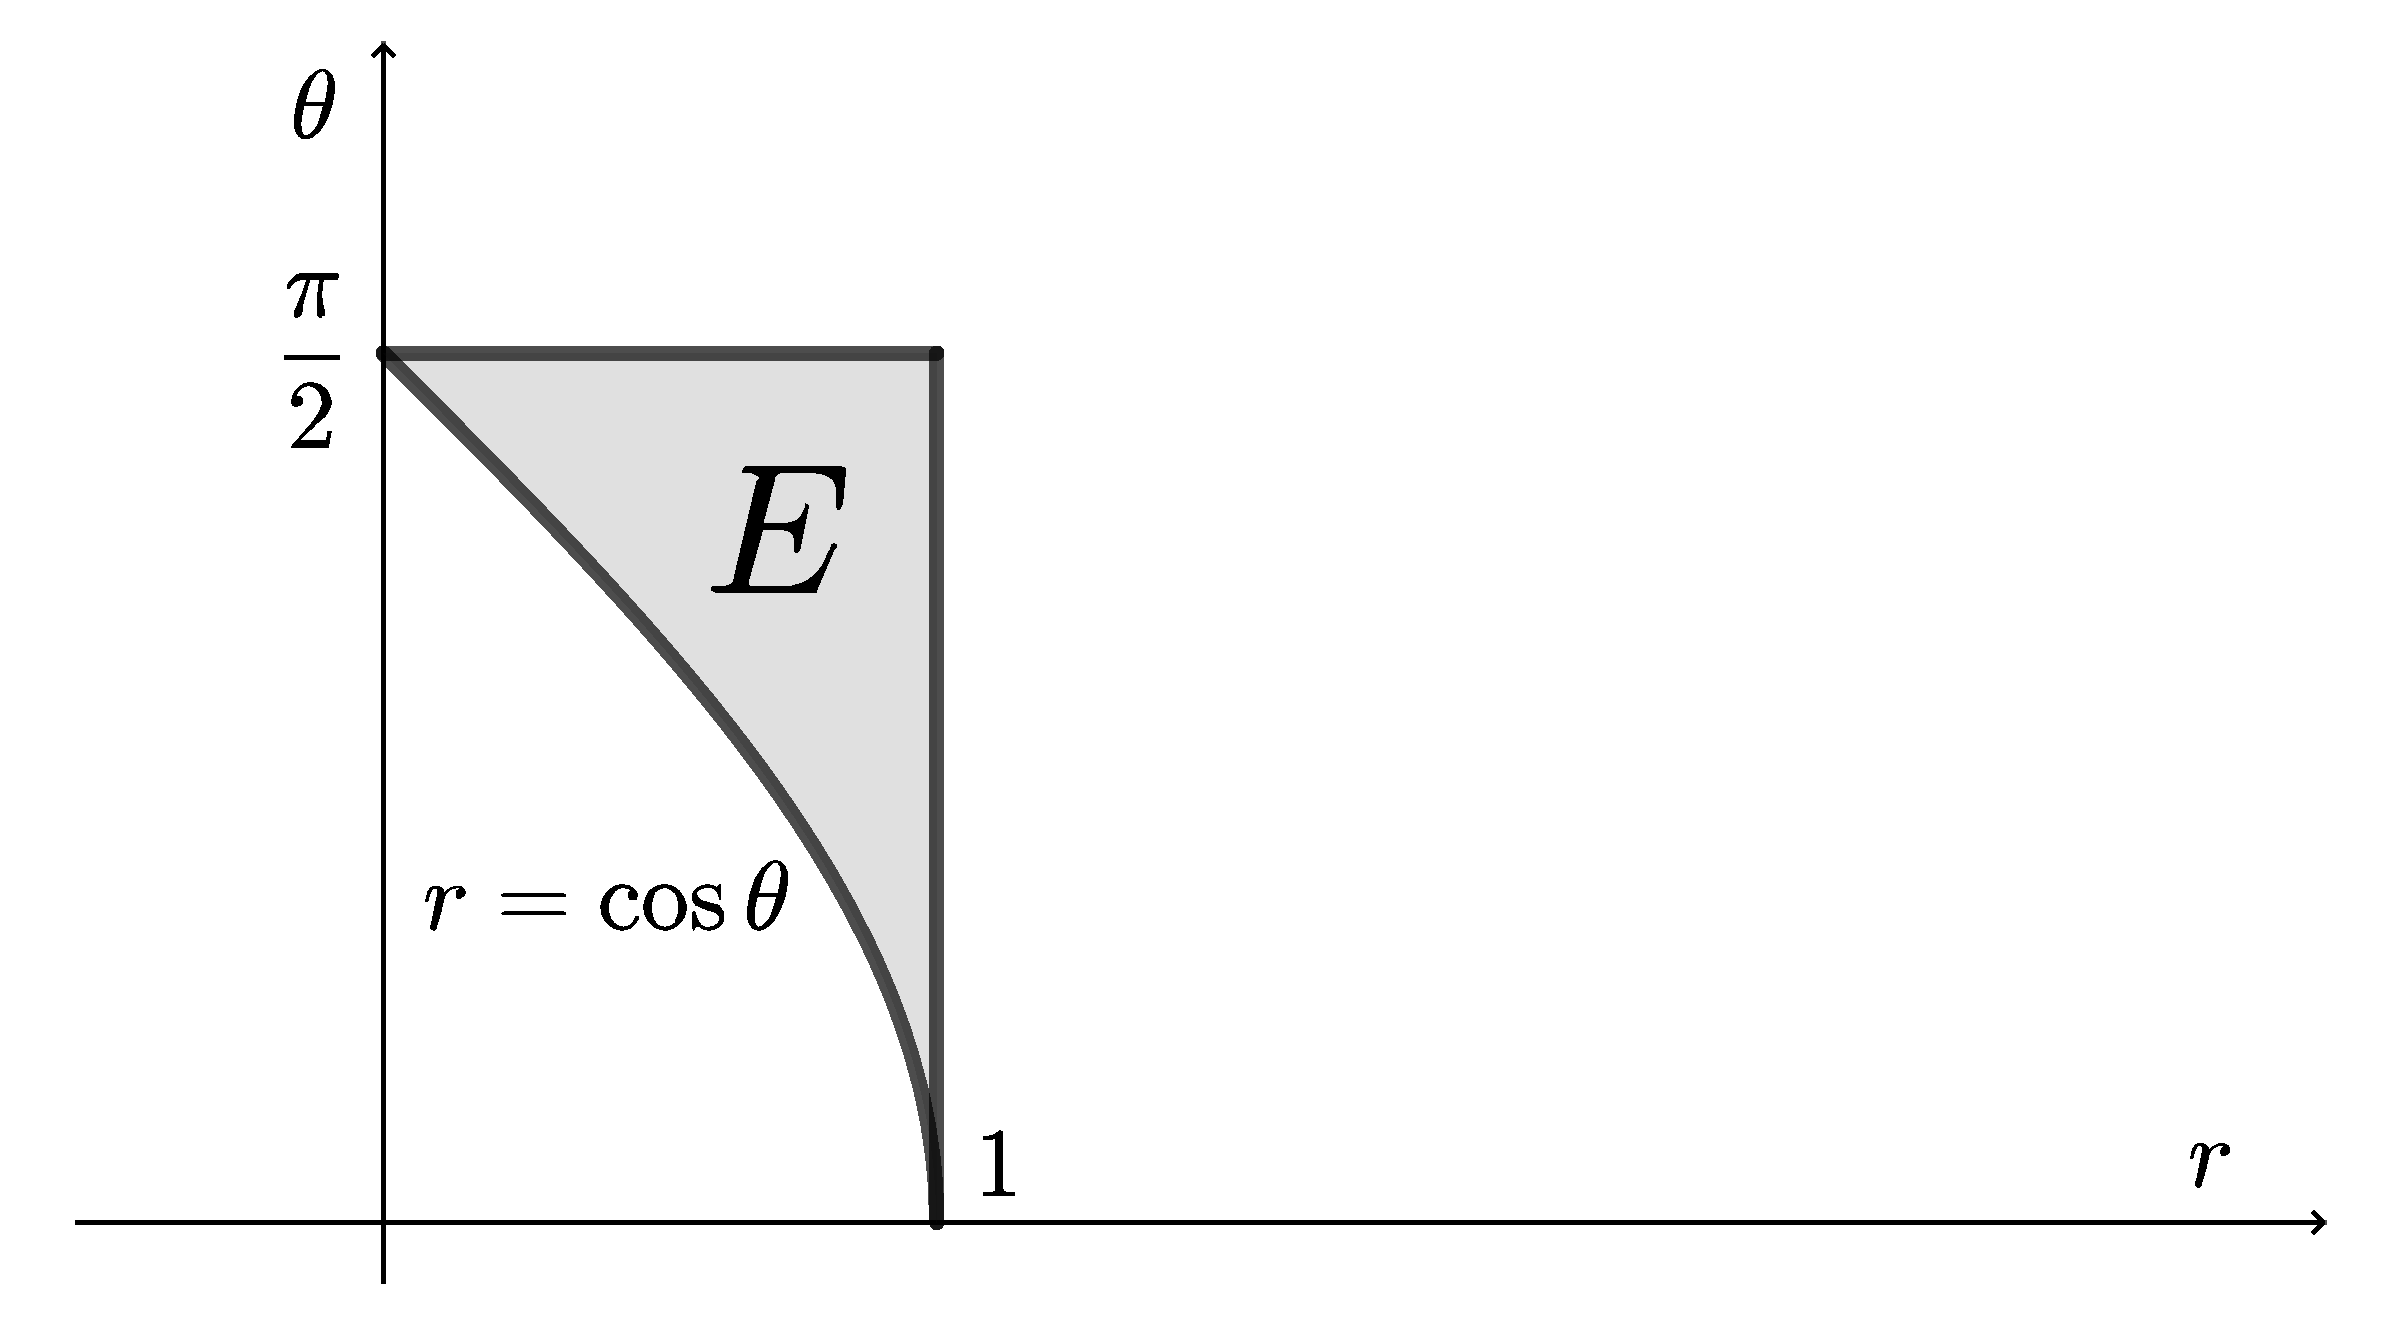
\includegraphics[height=4cm]{./pictures/no12p.pdf}
       \caption{$E=\Set{(r,\theta)  | 0 \leq \theta \leq \frac{\pi}{2}, \cos \theta \leq r \leq 1 }$}\label{fig:no12p}       
     \end{figure}

     変換のヤコビアンは $J(r,\theta)=r$ であるから,重積分は以下の様に書き直せる.
     \begin{align*}
       \iint_D \sqrt{x^2+y^2} \ dx dy 
       &= \iint_E r |J(r,\theta)|\ dr d\theta 
         = \int_{0}^{\frac{\pi}{2}} \left( \int_{\cos\theta}^{1} r^2 \ dr \right) d\theta\\
       &  = \int_{0}^{\frac{\pi}{2}} \left[\frac{1}{3}r^3\right]_{r=\cos\theta}^{r=1} \ d\theta
        =\frac{1}{3} \int_{0}^{\frac{\pi}{2}} \left(1-\cos^3 \theta \right) \ d\theta
       = \frac{\pi}{6}-\frac{2}{9}.
     \end{align*}

   \item 閉領域 $D$ を $xy$ 平面上に図示すると,図\ref{fig:no13}の通りである.
     \begin{figure}[h]
       \centering
       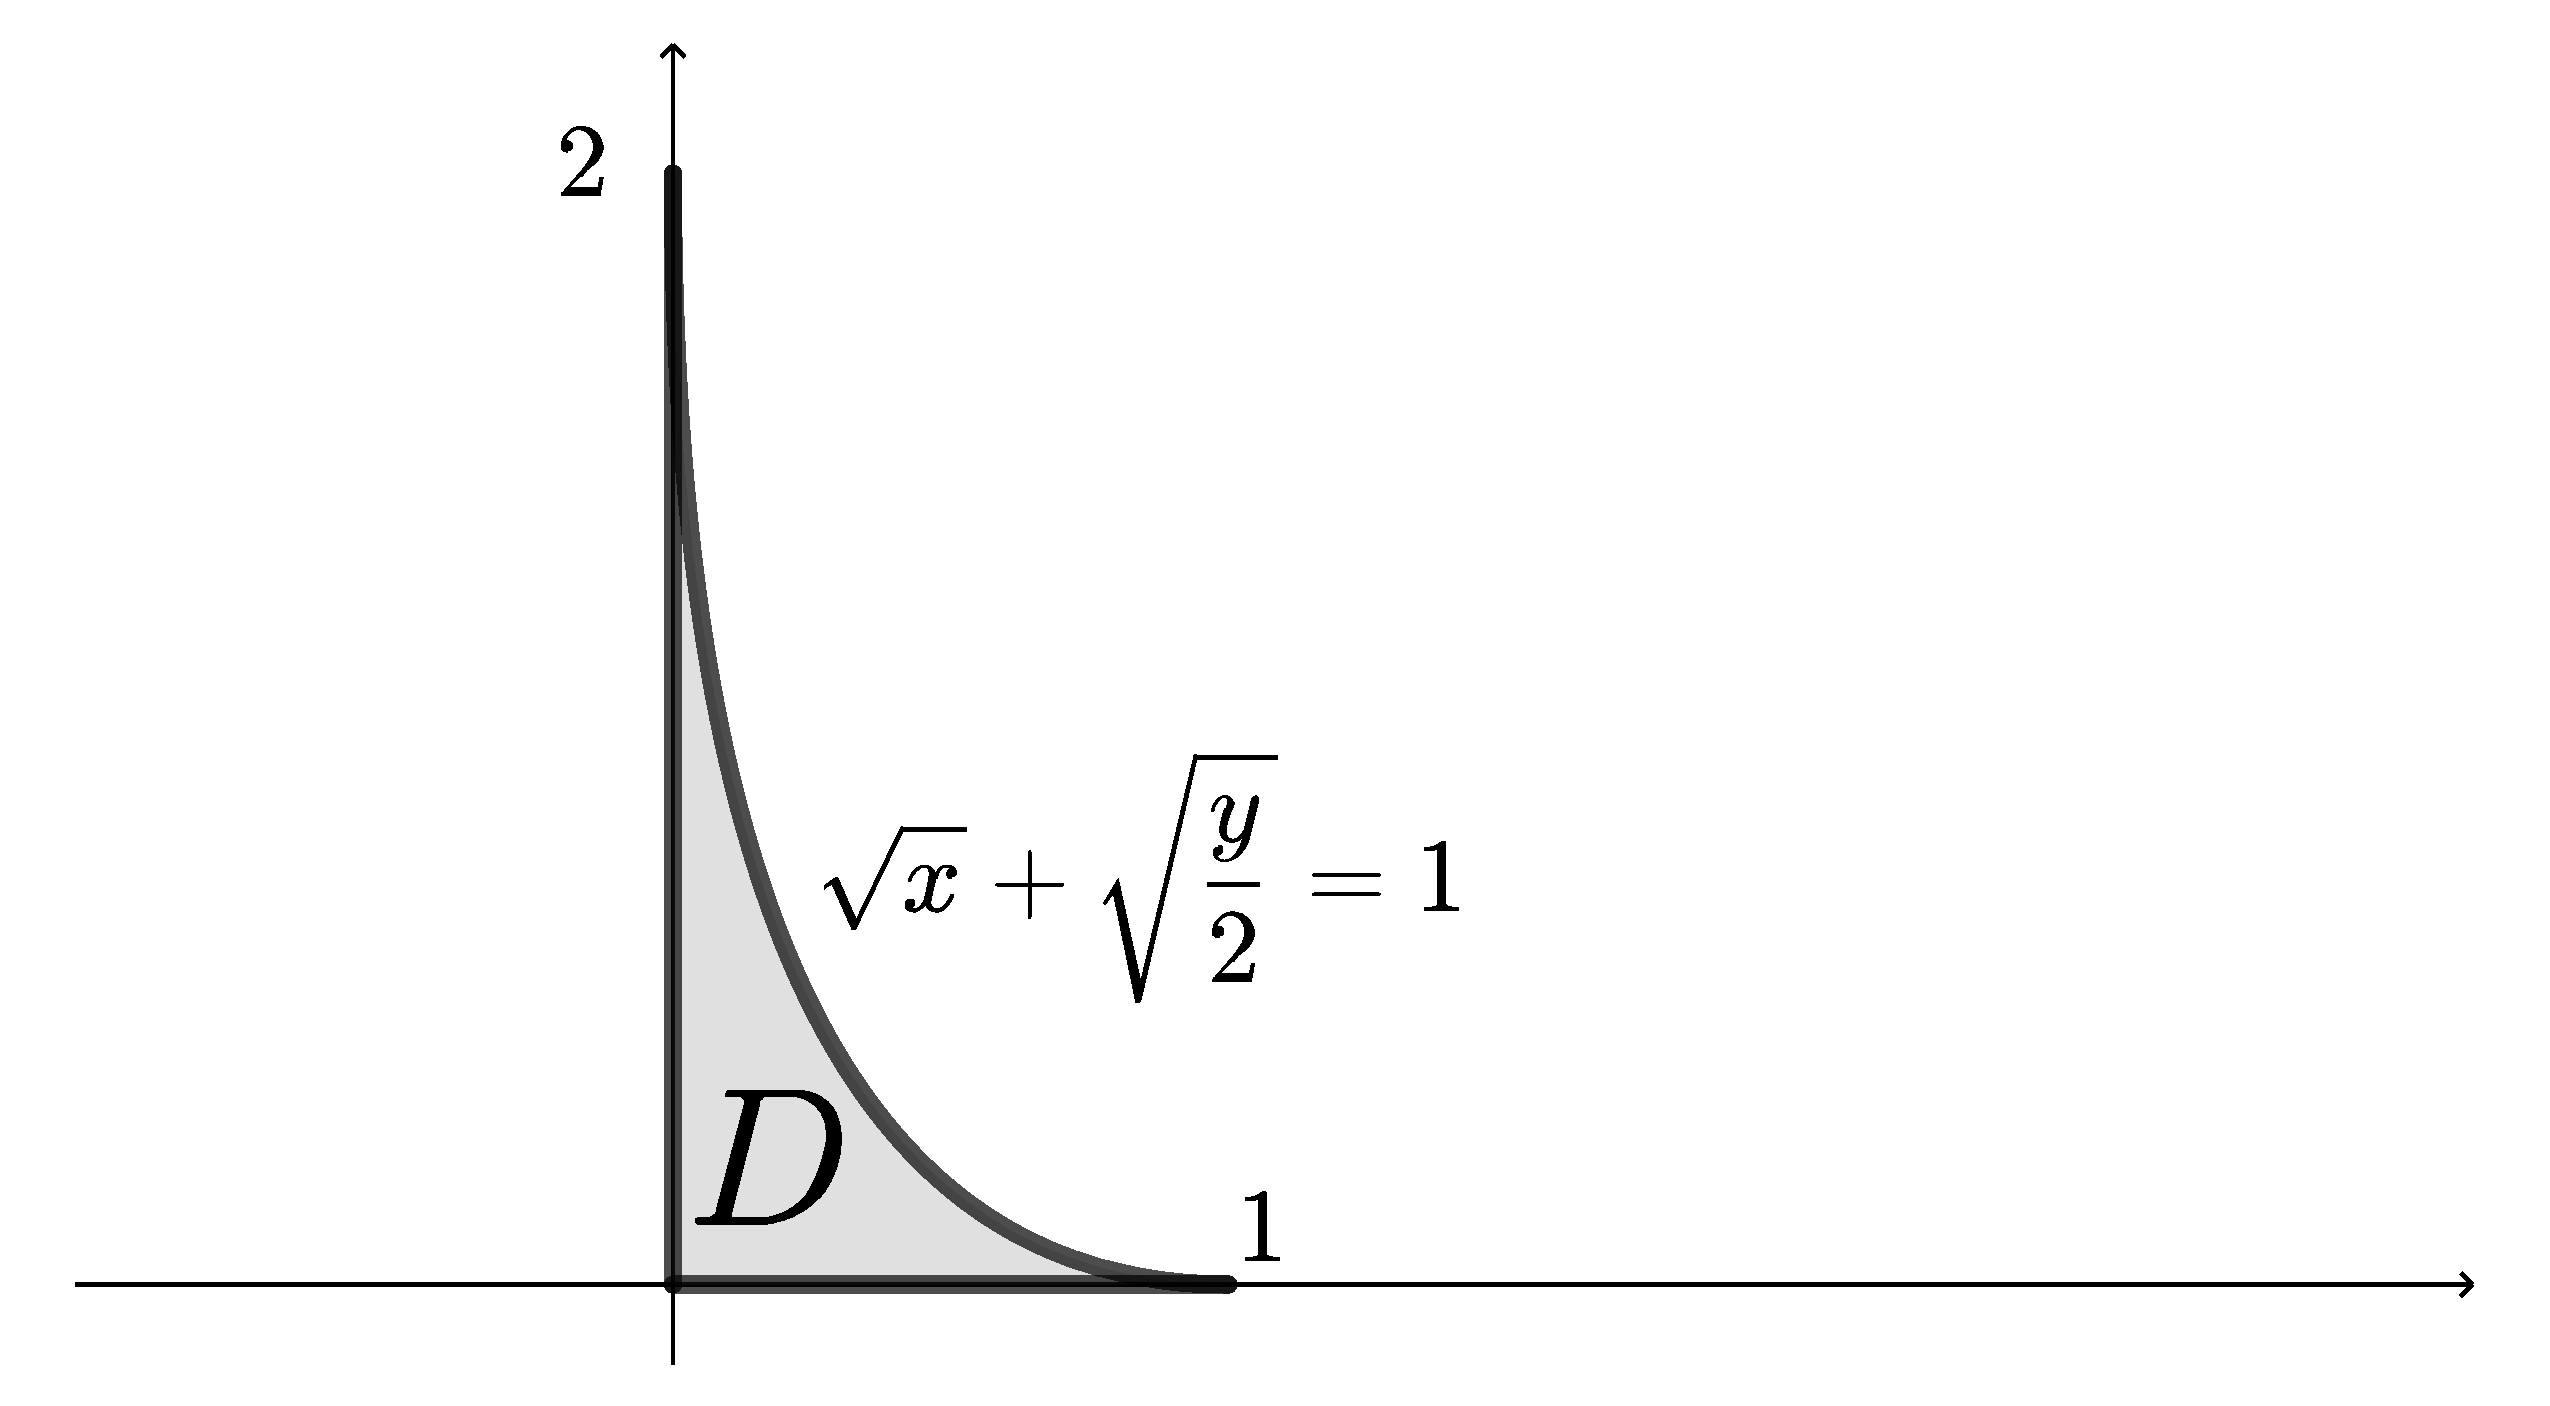
\includegraphics[height=4cm]{./pictures/no13.pdf}
       \caption{$D=\Set{ (x,y)  |  \sqrt{x} + \sqrt{\frac{y}{2}} \leq 1}$}\label{fig:no13}     
     \end{figure}

     変数変換
     \[
       x=u^2, \, y= 2v^2 \; (u \geq 0 , \, v \geq 0 )
     \]
     によって $uv$ 平面上の閉領域
     \[
       E= \Set{ (u,v)  |   0 \leq u \leq 1, \, 0 \leq v \leq 1-u }
     \]
     が $xy$ 平面上の閉領域 $D$ に変換される.閉領域 $E$ を $uv$ 平面に図
     示すると,図\ref{fig:no13uv}の通りである.
     \begin{figure}[h]
       \centering
       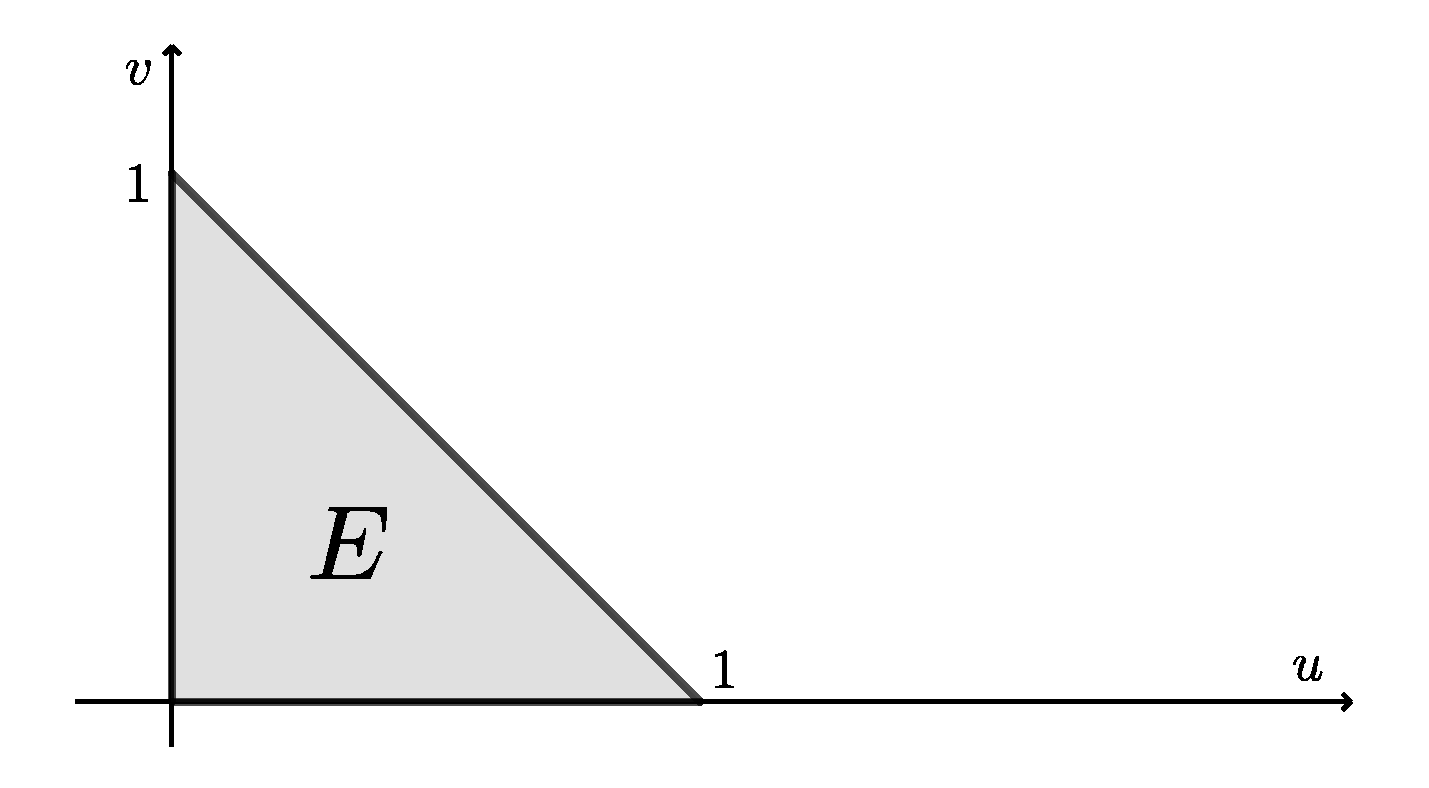
\includegraphics[height=4cm]{./pictures/no13uv.pdf}
       \caption{$E=\Set{(u,v)  |  0 \leq u \leq 1, \, 0 \leq v \leq 1-u}$}\label{fig:no13uv}
     \end{figure}

     変換のヤコビアンは
     \begin{spacing}{1.3}
       \[
         J(u,v) = \left|
           \begin{array}{cc}
             \frac{\partial x}{\partial u} & \frac{\partial x}{\partial v}\\
             \frac{\partial y}{\partial u} & \frac{\partial y}{\partial v}          
           \end{array}
         \right| = \left|
           \begin{array}{cc}
             2u & 0\\
             0 & 4v
           \end{array}
         \right| = 8uv
       \]
     \end{spacing}
     であるから,重積分は以下のように書き直せる.
       \begin{align*}
         \iint_D xy \ dx dy
         &= \iint_E 2u^2 v^2 |J(u,v)| \ du dv = 16 \int_{0}^{1} \left( \int_{0}^{1-u} u^3 v^3 \ dv \right) du\\
         &= 16 \int_{0}^{1} u^3 \left[\frac{1}{4} v^4\right]_{v=0}^{v=1-u} \ du
           =4 \int_{0}^{1} u^3(1-u)^4 \ du =\frac{1}{70}.
       \end{align*}

   \item 閉領域 $D$ を $xy$ 平面に図示すると,図\ref{fig:no14}の通りである.
     \begin{figure}[h]
       \centering
       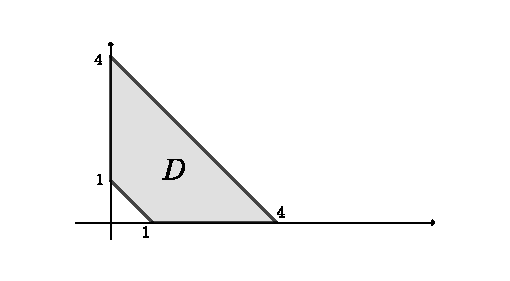
\includegraphics[height=4cm]{./pictures/no14.pdf}
       \caption{ $D=\Set{ (x,y)  |  1 \leq x+y \leq 4, \, 0 \leq x, \, 0 \leq y }$ }\label{fig:no14}
     \end{figure}
     
     これより $D$ は縦線集合として
     \[
       D=\Set{ (x,y)  |  0 \leq x \leq 4, \, \varphi_1(x) \leq y \leq \varphi_2(x) }
     \]
     と表せる.ただし,ここで
     \[
       \varphi_1(x) = \left\{
         \begin{array}{cl}
           -x+1 & (x \leq 1)\\
           0 & (1 \leq x)
         \end{array}
       \right. , \quad \varphi_2(x) = -x+4
     \]
     である.これより重積分は以下のように2つの累次積分の和に書き直せる.
     \begin{align*}
       \iint_D \frac{x^2+y^2}{(x+y)^3} dx dy
       &= \int_{0}^{1} \left( \int_{\varphi_1(x)}^{\varphi_2(x)} \frac{x^2+y^2}{(x+y)^3} \ dy \right)dx\\
       &= \int_{0}^{1} \left( \int_{-x+1}^{-x+4} \frac{x^2+y^2}{(x+y)^3} \  dy \right)dx 
         + \int_{1}^{4} \left( \int_{0}^{-x+4} \frac{x^2+y^2}{(x+y)^3} \  dy \right) dx.
     \end{align*}
     被積分関数を $y$ の1変数関数と見なして部分分数に分解すると
     \[
       \frac{x^2+y^2}{(x+y)^3} = \frac{1}{x+y}-\frac{2x}{(x+y)^2} + \frac{2x^2}{(x+y)^3}
     \]
     である.よって,
     \begin{align*}
       & \int_{0}^{1} \left( \int_{-x+1}^{-x+4} \frac{x^2+y^2}{(x+y)^3} \ dy \right) dx\\
       & \quad = \int_{0}^{1} \left( \int_{-x+1}^{-x+4}\frac{dy}{x+y} -2x \int_{-x+1}^{-x+4} \frac{dy}{(x+y)^2}
         + 2x^2 \int_{-x+1}^{-x+4} \frac{dy}{(x+y)^3} \right) dx\\
       & \quad = \int_{0}^{1}\left(\Big[ \log |x+y| \Big]_{y=-x+1}^{y=-x+4}
         + 2x\left[\frac{1}{x+y}\right]_{y=-x+1}^{y=-x+4}
         -x^2 \left[ \frac{1}{(x+y)^2}\right]_{y=-x+1}^{y=-x+4} \right) dx\\
       & \quad = \int_{0}^{1} \left( \frac{15}{16}x^2-\frac{3}{2} x + 2\log 2 \right) \ dx=-\frac{7}{16}+2\log 2
     \end{align*}
     を得る.全く同様にして
     \[
       \int_{1}^{4}\left( \int_{0}^{-x+4} \frac{x^2+y^2}{(x+y)^3}\  dy \right) dx = \frac{39}{16}-2\log 2
     \]
     が得られるので,これらを合わせて以下を得る.
     \[
       \iint_{D} \frac{x^2+y^2}{(x+y)^3}dxdy = \left(-\frac{7}{16}+2\log 2\right)
       + \left(\frac{39}{16}-2\log2\right) = 2.
     \]
 

   \item 閉領域 $D$ を $xy$ 平面に図示すると,図\ref{fig:no15}の通りである.
     \begin{figure}[h]
       \centering
       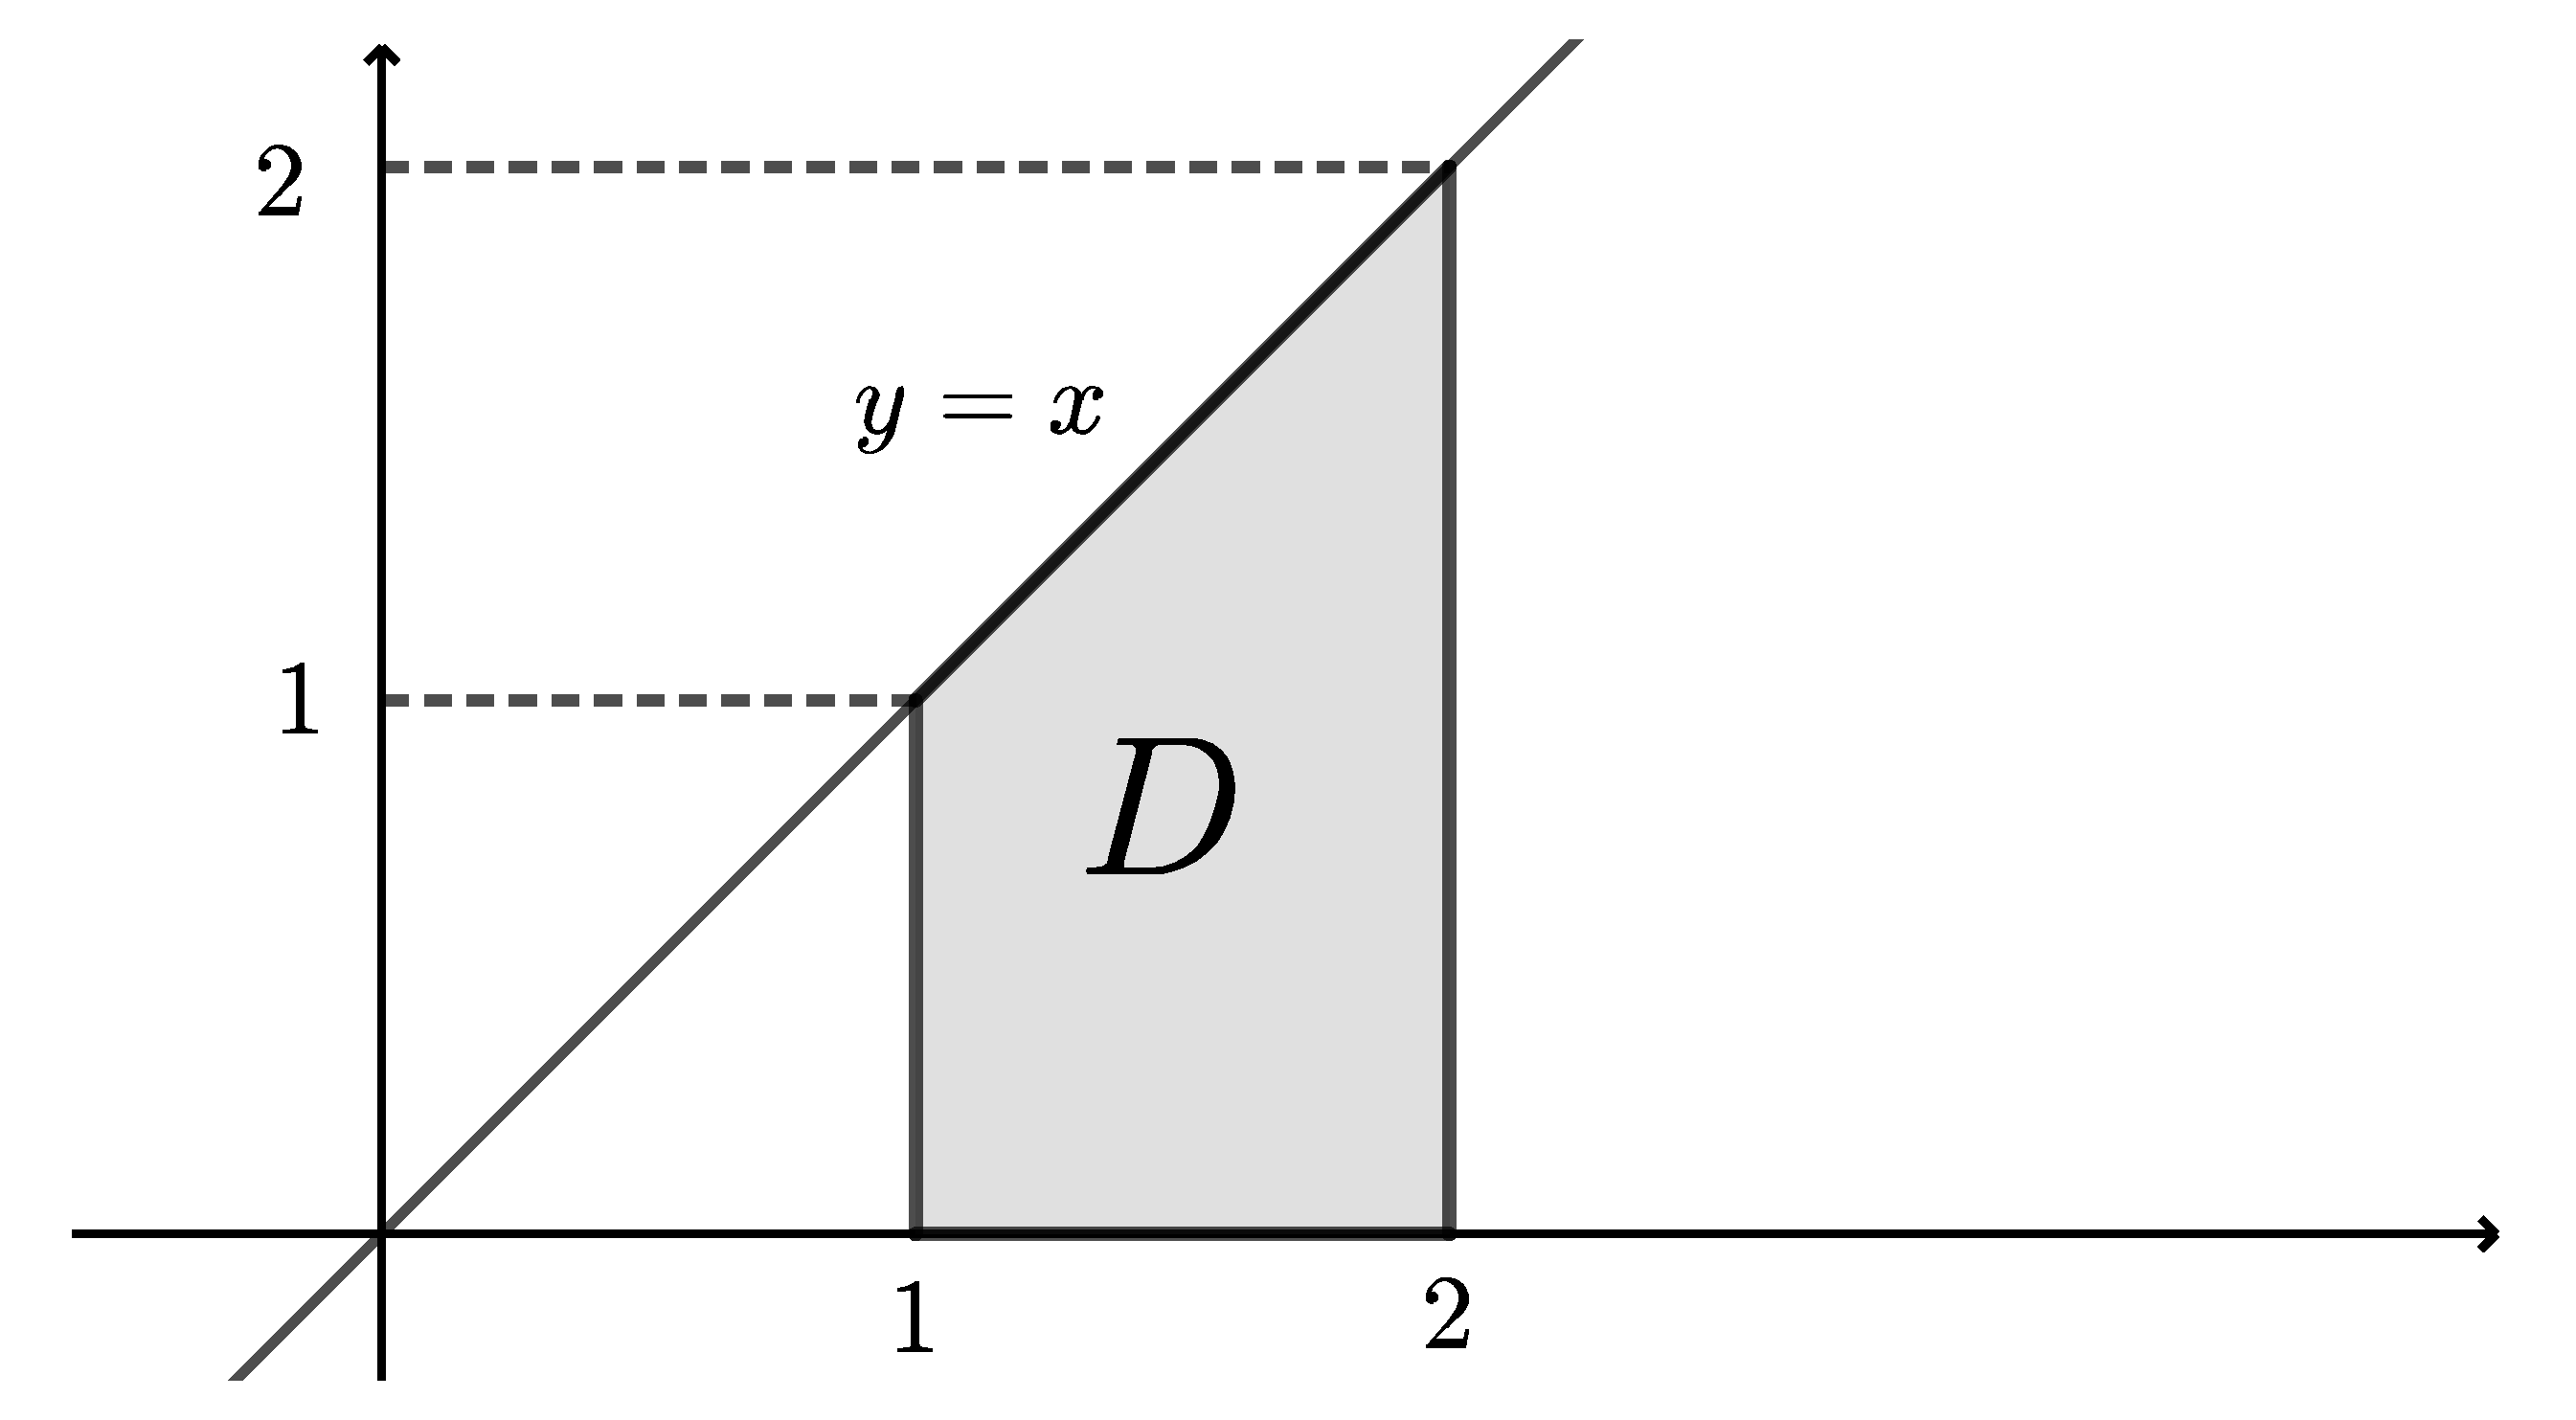
\includegraphics[height=4cm]{./pictures/no15.pdf}
       \caption{ $D=\Set{(x,y)  |  1 \leq x \leq 2, \, 0 \leq y \leq x }$}\label{fig:no15}
     \end{figure}
     
     $D$ を縦線集合と見なして,重積分は以下のように書き直せる.
     \[
       \iint_D \frac{x+y}{x^2} e^{\frac{y}{x}} \ dx dy 
       = \int_{1}^{2} \left( \int_{0}^{x} \frac{x+y}{x^2}e^{\frac{y}{x}}\  dy \right)dx
       =\int_{1}^{2} \left[\frac{y}{x} e^{\frac{y}{x}} \right]_{y=0}^{y=x} \ dx
       =\int_{1}^{2} e \ dx = e.
     \]
     
   \item 集合 $D$ は閉領域ではないのでこれは広義積分である.自然数 $n$ に対して
     \[
       D_n = \Set{(x,y) | \frac{1}{n} \leq x \leq 1, \, \frac{1}{n} \leq y \leq 1}
     \]
     とすると,$\Set{D_n}$ は $D$ の増加近似列であり,これを図示すると図\ref{fig:no16}の通りである.
     \begin{figure}[h]
       \centering
       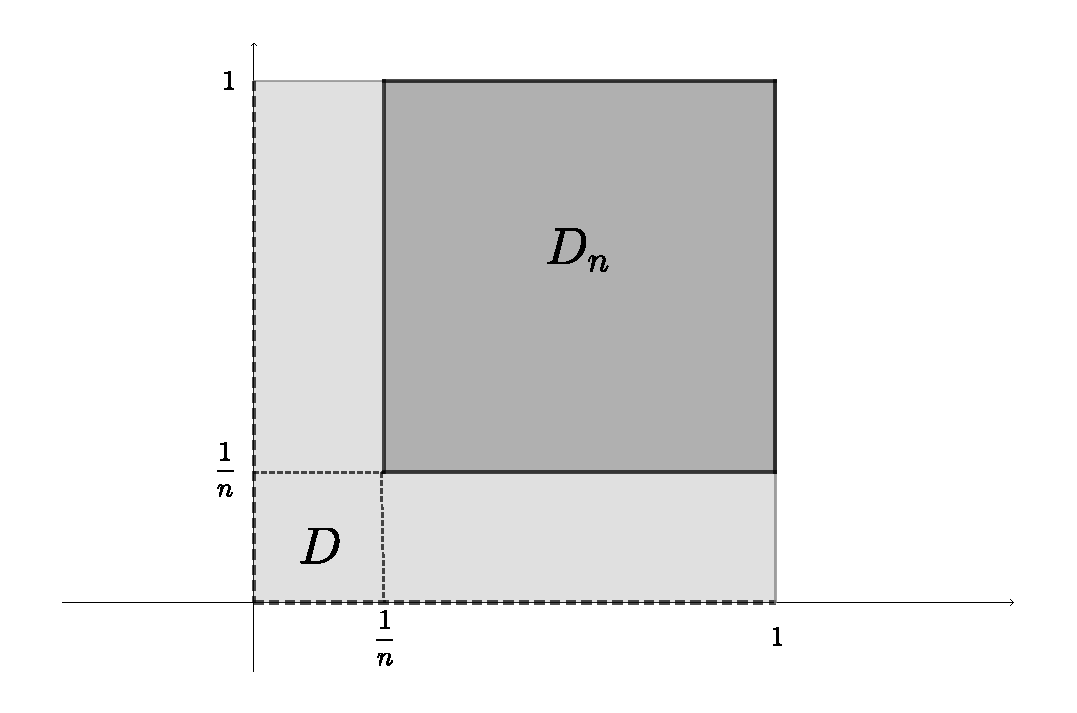
\includegraphics[height=4cm]{./pictures/no16.pdf}
       \caption{ $D_n=\Set{(x,y)  |  \frac{1}{n} \leq x \leq 1, \, \frac{1}{n} \leq y \leq 1}$}\label{fig:no16}
     \end{figure}


     $(x,y) \in D$ に対して $\frac{1}{x+y} >0$ であるから,極限
     \[
       \lim_{n \to \infty} \iint_{D_n} \frac{dx dy}{x+y}
     \]
     が存在すれば広義積分は収束し,その極限値が求める広義積分の値である.
     各 $D_n$ は横線集合と見なせるので $D_n$ 上の重積分は以下のように書
     き直せる.
     \begin{align*}
       \iint_{D_n} \frac{dx dy}{x+y} 
       &= \int_{\frac{1}{n}}^{1} \left( \int_{\frac{1}{n}}^{1} \frac{dx}{x+y}\right) dy
         = \int_{\frac{1}{n}}^{1} \Big[ \log |x+y| \Big]_{x=\frac{1}{n}}^{x=1}  dy\\
       &= \int_{\frac{1}{n}}^{1} \left( \log\left(y+1\right)-\log\left(y+\frac{1}{n}\right)\right) dy\\
       &= \left[ \left( y+1 \right) \log \left(y+1\right) -1 -\left( y+\frac{1}{n}\right)\log\left(y+\frac{1}{n}\right)
         +\frac{1}{n}\right]_{\frac{1}{n}}^{1}\\
       &= 2\log 2 - 2\left(1+\frac{1}{n}\right) \log \left(1+\frac{1}{n}\right) + \frac{2}{n}\log\frac{2}{n}.
     \end{align*}
     ここで,$t=\frac{2}{n}$ とおくと$n \to \infty$ のとき $t \to +0$ であるから,ロピタルの定理より
     \[
       \lim_{n \to \infty} \frac{2}{n} \log \frac{2}{n} = \lim_{t \to +0} t \log t = \lim_{t \to +0} \frac{\log t}{\frac{1}{t}}
       = \lim_{t \to +0} \frac{\frac{1}{t}}{-\frac{1}{t^2}} = -\lim_{t \to +0} t = 0
     \]
     である.これより,以下を得る.
     \[
       \iint_{D} \frac{dx dy}{x+y} = \lim_{n \to \infty} \iint_{D_n} \frac{dx dy}{x+y} = 2 \log 2.
     \]
 


   \item 集合 $D$ は有界ではないのでこれは広義積分である.自然数 $n$ に対して
     \[
       D_n =\Set{ (x,y) |  0 \leq x \leq n, \, 0 \leq y \leq n }
     \]
     とすると,$\Set{D_n}$ は $D$ の増加近似列であり,これを図示すると図\ref{fig:no17}の通りである.
     \begin{figure}[h]
       \centering
       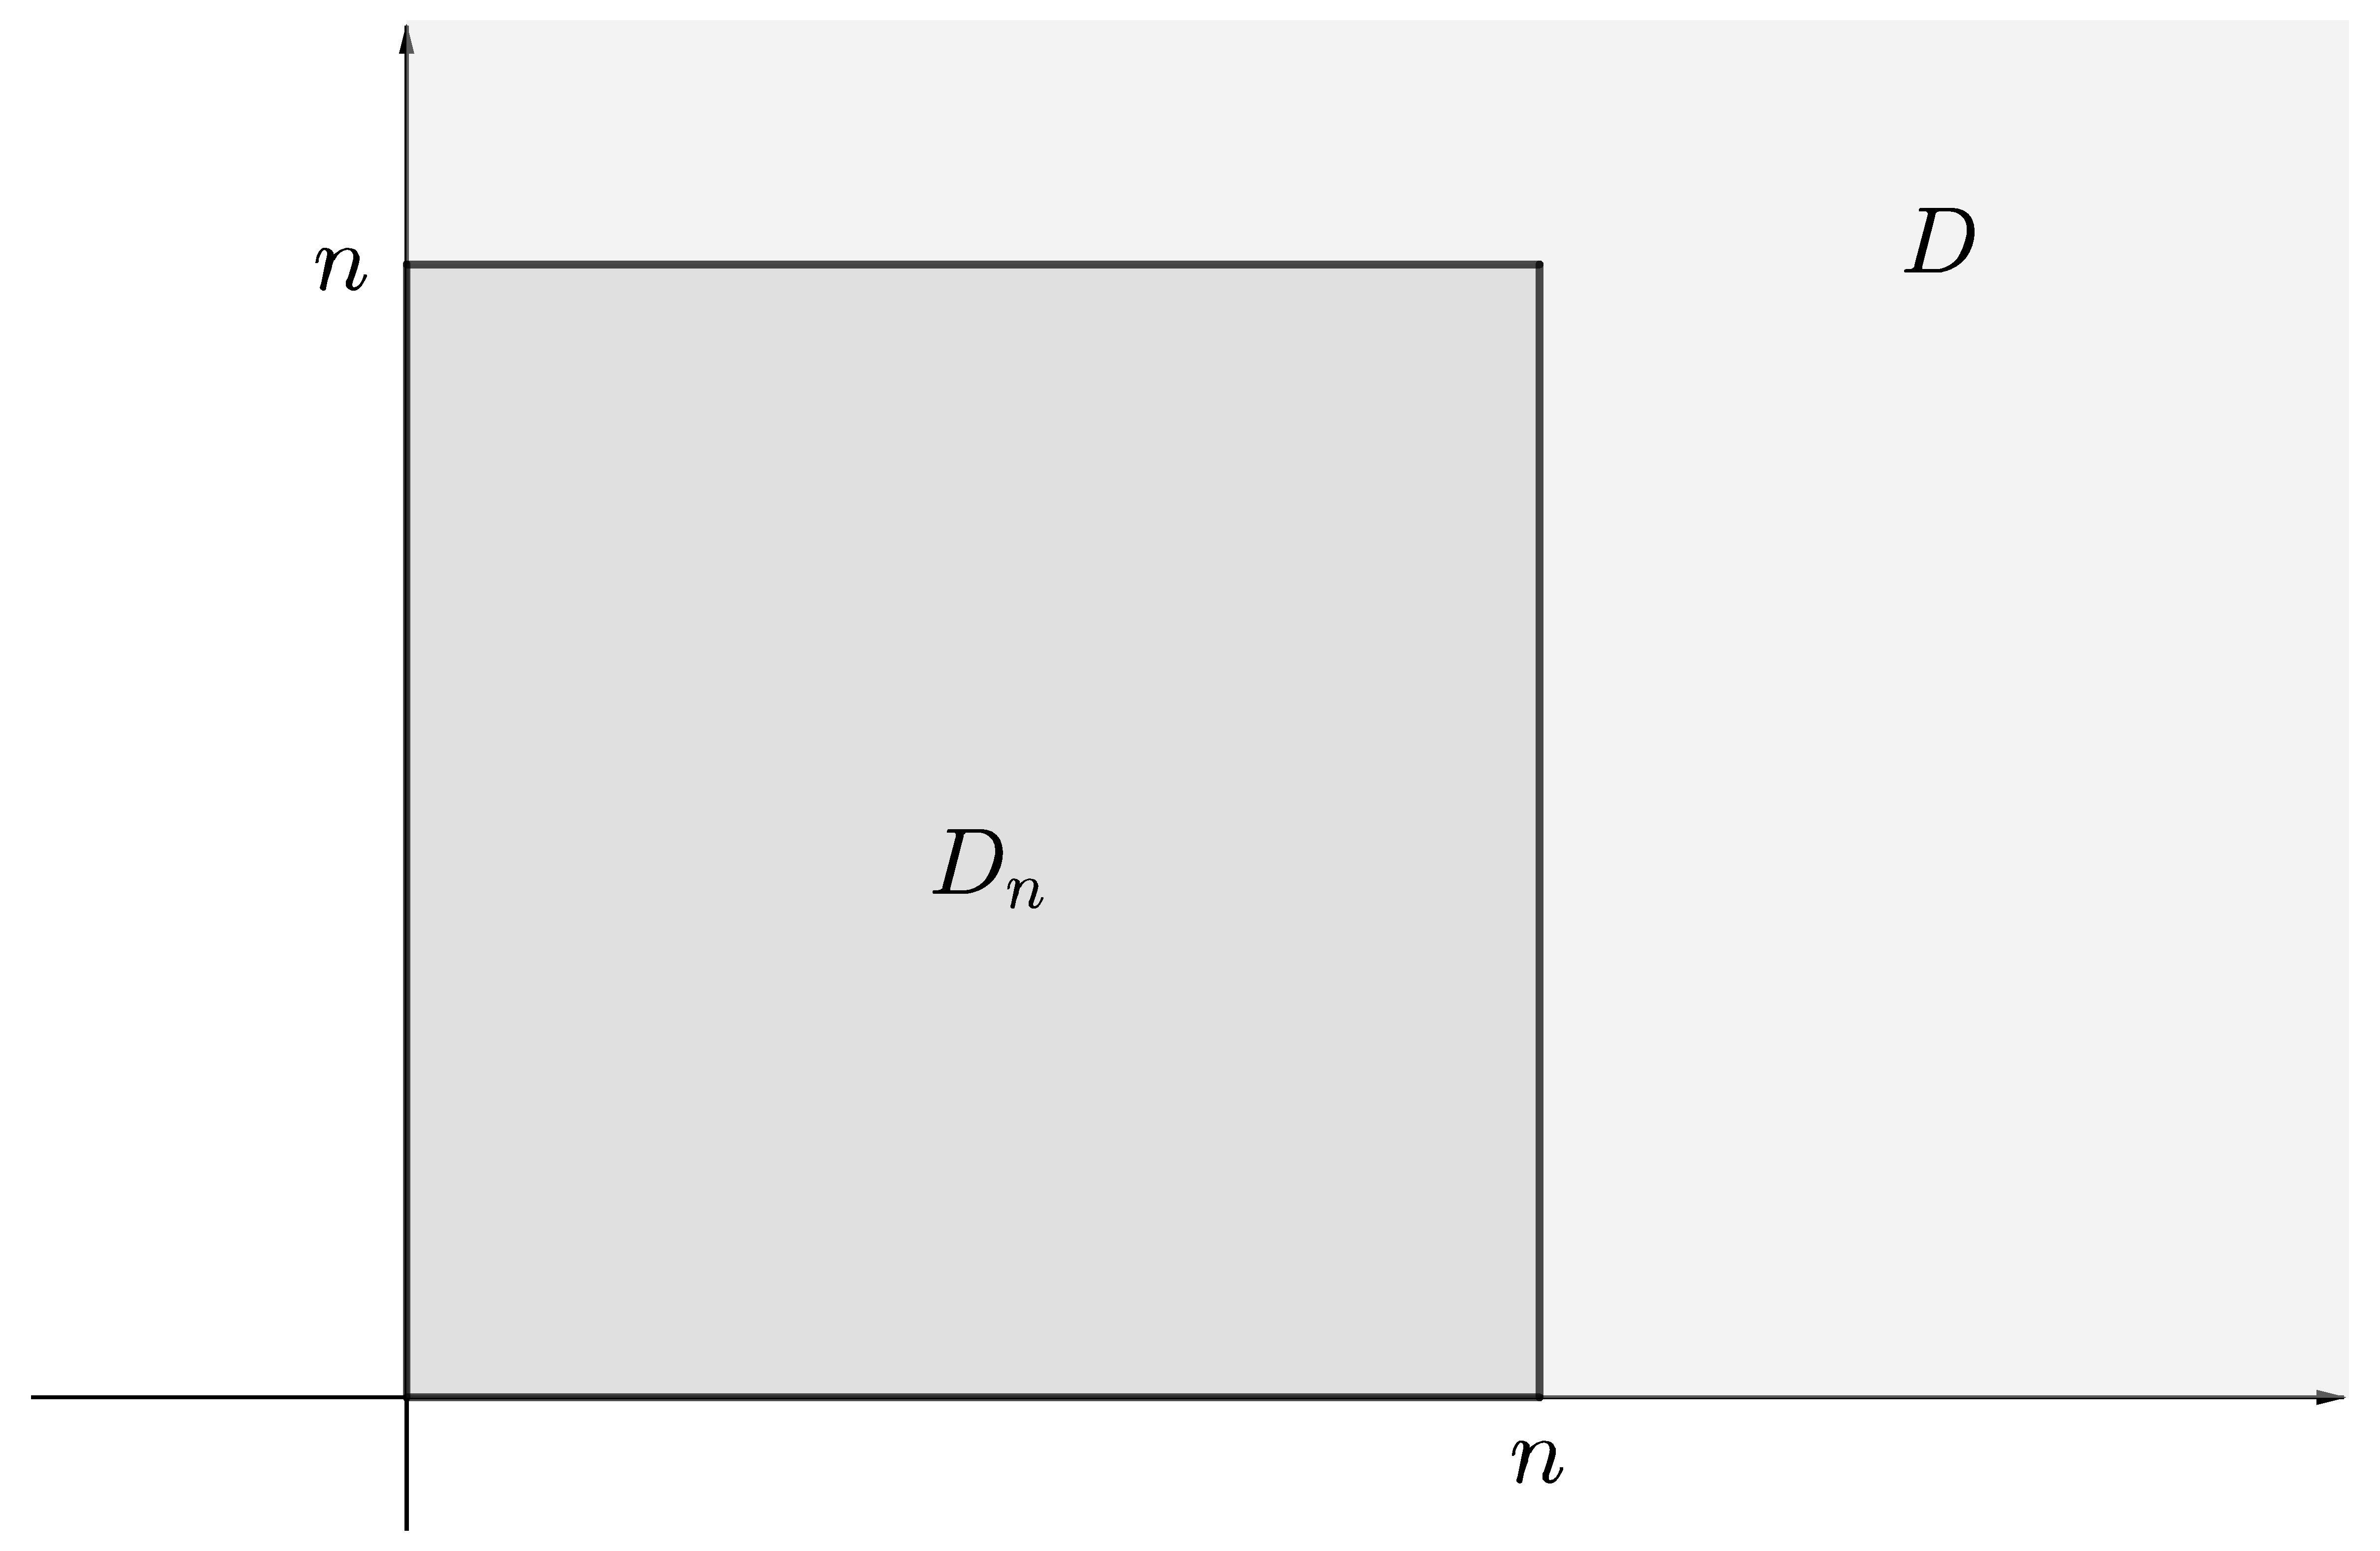
\includegraphics[height=4cm]{./pictures/no17.pdf}
       \caption{ $D_n=\Set{(x,y)  |  0 \leq x \leq n, \, 0 \leq y \leq n}$}\label{fig:no17}
     \end{figure}

     $(x,y) \in D$ に対して $e^{-x-y}
     \geq 0 $ であるから,極限
     \[
       \lim_{n \to \infty} \iint_{D_n} e^{-x-y} dx y
     \]
     が存在すれば広義積分は収束し,その極限値が求める広義積分の値である.
     各 $D_n$ は横線集合と見なせるので $D_n$ 上の重積分は以下のように書き
     直せる.
     \begin{align*}
       \iint_{D_n} e^{-x-y}\ dx dy
       &= \int_{0}^{n} \left(\int_{0}^{n} e^{-x-y} \  dx \right) dy
         = \int_{0}^{n} e^{-y} \left[-e^{-x}\right]_{0}^{n} dy = (1-e^{-n})\int_{0}^{n}e^{-y} dy\\
       &=(1-e^{-n})^2.
     \end{align*}
     よって,これより以下を得る.
     \[
       \iint_D e^{-x-y}\ dxdy = \lim_{n \to \infty} \int_{D_n} e^{-x-y} \ dxdy 
       = \lim_{n \to \infty} \left(1-e^{-n}\right)^2 =1.
     \]

   \item 集合 $D$ は閉領域ではないのでこれは広義積分である.自然数 $n$ に対して
     \[
       D_n=\Set{(x,y) | \frac{1}{n} \leq x \leq 1, \, 0 \leq y \leq 1}
     \]
     とすると,$\Set{D_n}$ は $D$ の増加近似列であり,これを図示すると図\ref{fig:no18}の通りである.
     \begin{figure}[h]
       \centering
       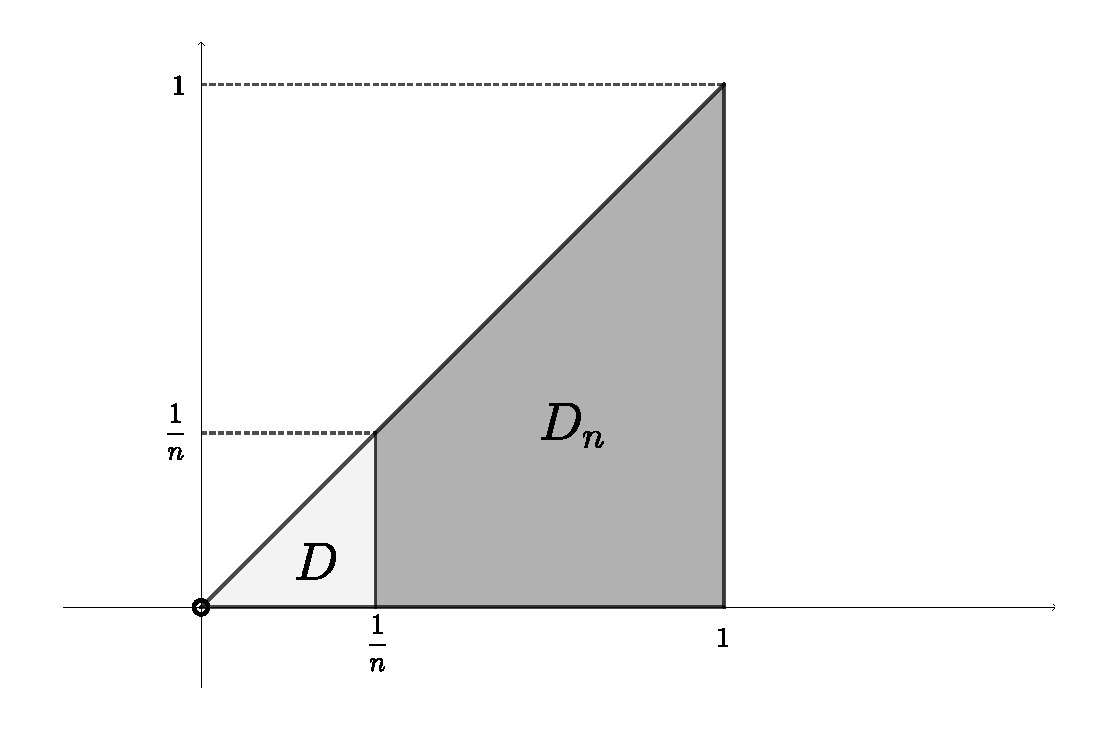
\includegraphics[height=4cm]{./pictures/no18.pdf}
       \caption{ $D_n=\Set{(x,y)  |  \frac{1}{n} \leq x \leq 1, \, 0 \leq y \leq 1}$}\label{fig:no18}
     \end{figure}

     $(x, y) \in D$ に対して $e^{\frac{y}{x}}>0$ であるから,極限
     \[
       \lim_{n \to \infty} \iint_{D_n} e^{\frac{x}{y}}\  dx dy
     \]
     が存在すれば広義積分は収束し,その極限値が求める広義積分の値である.
     各 $D_n$ は縦線集合と見なせるので $D_n$ 上の重積分は以下のように書
     き直せる.
     \begin{align*}
       \iint_{D_n} e^{\frac{y}{x}}\ dx dy
       &= \int_{\frac{1}{n}}^{1} \left( \int_{0}^{x} e^{\frac{y}{x}}\ dy \right) dx
         =\int_{\frac{1}{n}}^{1}\left[xe^{\frac{y}{x}}\right]_{y=0}^{y=x} dx
         =(e-1) \int_{\frac{1}{n}}^{1}x \ dx\\
       &= \frac{e-1}{2}\left( 1- \frac{1}{n^2}\right).
     \end{align*}
     よって,これより以下を得る.
     \[
       \iint_{D} e^{\frac{y}{x}}\ dx dy = \lim_{n \to \infty} \frac{e-1}{2}\left(1-\frac{1}{n^2}\right) = \frac{e-1}{2}.
     \]
 

   \item 集合 $D$ は閉領域ではないのでこれは広義積分である.自然数 $n$ に対して
     \[
       D_n=\Set{ (x,y) | \frac{1}{n} \leq x \leq 1, \, 0 \leq y \leq 1}
     \]
     とすると,$\Set{D_n}$ は $D$ の増加近似列であり,これを図示すると図\ref{fig:no19}の通りである.
     \begin{figure}[h]
       \centering
       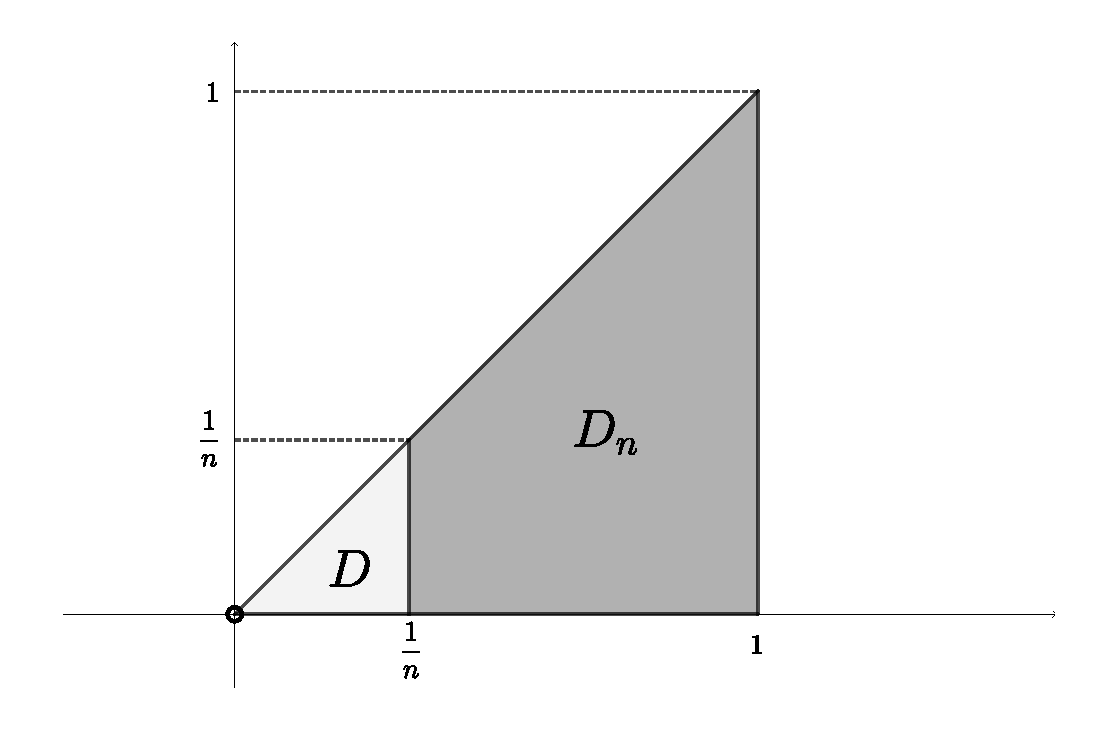
\includegraphics[height=4cm]{./pictures/no19.pdf}
       \caption{ $D_n=\Set{(x,y)  |  \frac{1}{n} \leq x \leq 1, \, 0 \leq y \leq 1}$}\label{fig:no19}
     \end{figure}
     
     $(x,y) \in D$ に対し
     て $\frac{x+y}{x^2+y^2} >0$ であるから,極限
     \[
       \lim_{n \to \infty} \iint_{D_n} \frac{x+y}{x^2+y^2} \ dx dy
     \]
     が存在すれば広義積分は収束し,その極限値が求める広義積分の値である.
     各 $D_n$ は縦線集合と見なせるので $D_n$ 上の重積分は以下のように書
     き直せる.
     \begin{align*}
       \iint_{D_n} \frac{x+y}{x^2+y^2} \ dx dy
       &= \int_{\frac{1}{n}}^{1}\left( \int_{0}^{x} \frac{x+y}{x^2+y^2} \ dy \right) dx\\
       &= \int_{\frac{1}{n}}^{1} \left( x \int_{0}^{x} \frac{dy}{x^2+y^2} 
         + \frac{1}{2} \int_{0}^{x} \frac{2y}{x^2+y^2}\ dy\right) dx\\
       &= \int_{\frac{1}{n}}^{1}\left(\left[ \tan^{-1}\frac{y}{x}\right]_{y=0}^{y=x} 
         + \frac{1}{2} \Big[ \log(x^2+y^2) \Big]_{y=0}^{y=x} \right) dx\\
       &=\left(\frac{\pi}{4} + \frac{1}{2}\log 2 \right)\int_{\frac{1}{n}}^{1} dx
       = \left( \frac{\pi}{4}+\frac{1}{2}\log 2\right) \left( 1-\frac{1}{n}\right).
     \end{align*}
     よって,これより以下を得る.
     \[
       \iint_{D}\frac{x+y}{x^2+y^2} \ dx dy 
       = \lim_{n \to \infty} \left( \frac{\pi}{4}+\frac{1}{2}\log 2\right)\left(1-\frac{1}{n}\right)
       =\frac{\pi}{4}+\frac{1}{2}\log 2.
     \]
       
   \item 集合 $D$ は閉領域ではないのでこれは広義積分である.自然数 $n$ に対して
     \[
       D_n=\Set{ (x,y)  |  0 \leq x \leq 1, \, 0 \leq y \leq x-\frac{1}{n}}
     \]
     とおくと,$\Set{D_n}$ は $D$ の増加近似列であり,これを図示すると図\ref{fig:no20}の通りである.
     \begin{figure}[h]
       \centering
       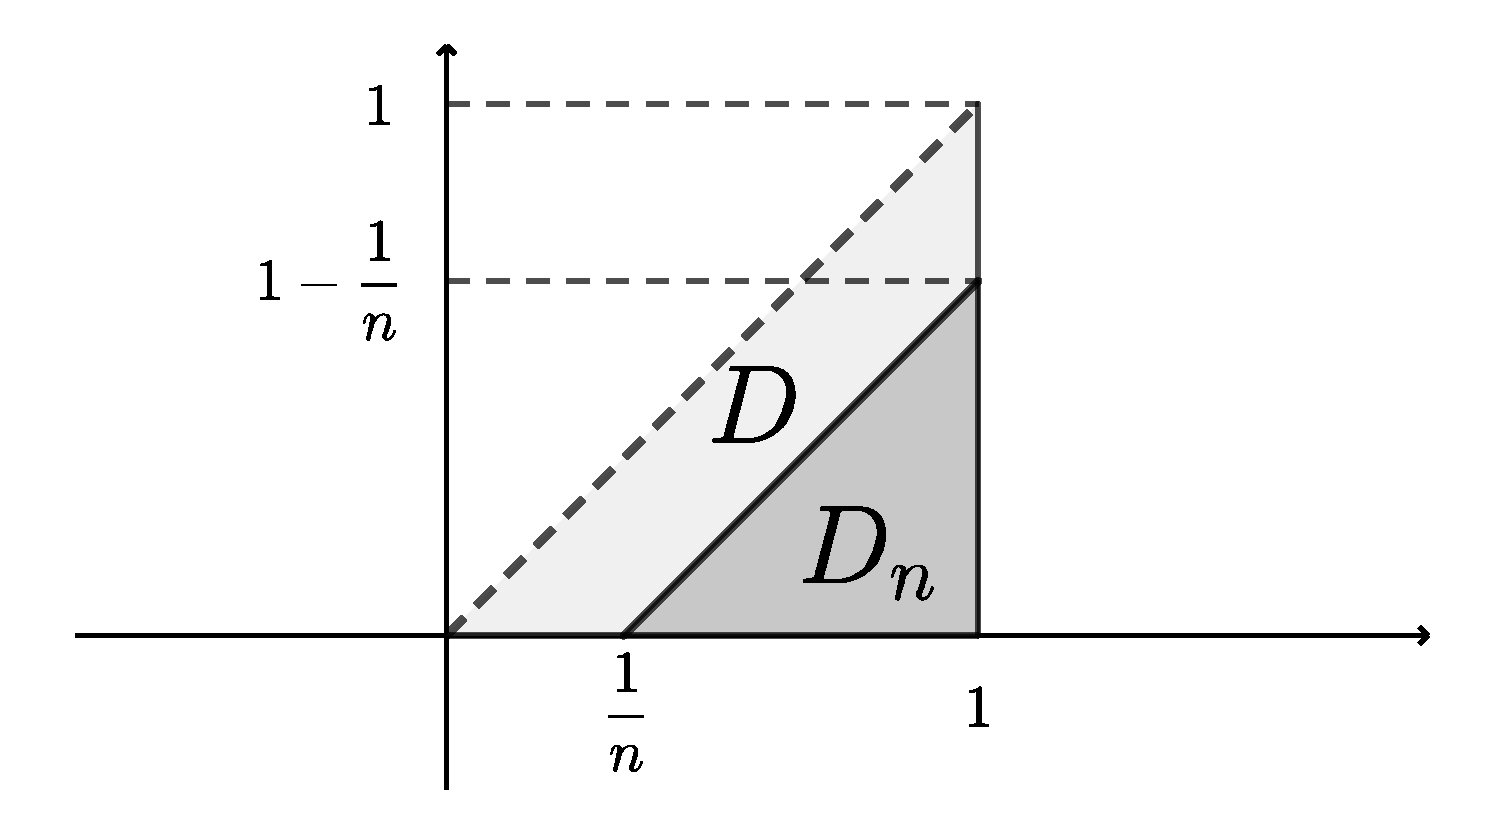
\includegraphics[height=4cm]{./pictures/no20.pdf}
       \caption{ $D_n=\Set{(x,y)  |  0 \leq x \leq 1, \, 0 \leq y \leq 1-\frac{1}{n}}$}\label{fig:no20}
     \end{figure}

     $(x,y) \in D$ 対して $\frac{1}{\sqrt{x^2-y^2}} \geq0$ であるから,極限
     \[
       \lim_{n \to \infty} \iint_{D_n} \frac{dxdy}{\sqrt{x^2-y^2}}
     \]
     が存在すれば広義積分は収束し,その極限値が求める広義積分の値である.
     各 $D_n$ は縦線集合と見なせるので $D_n$ 上の重積分は以下のように書き
     直せる.
     \begin{align*}
       \iint_{D_n} \frac{dxdy}{\sqrt{x^2-y^2}}
       &= \int^{1}_{\frac{1}{n}}
         \left( \int_{0}^{x-\frac{1}{n}} \frac{1}{\sqrt{x^2-y^2}} \ dy \right) dx
         = \int^{1}_{\frac{1}{n}} \left[ \sin^{-1} \frac{y}{x} \right]_{y={\frac{1}{n}}}^{y=x-\frac{1}{n}} \ dx\\
       &= \int^{1}_{\frac{1}{n}} \sin^{-1}\left(1-\frac{1}{nx}\right) dx
         = \left[ x \sin^{-1} \left(1-\frac{1}{nx}\right) - \frac{ \sqrt{2nx-1}}{n} \right]^{1}_{\frac{1}{n}}\\
       &= \sin^{-1}\left(1-\frac{1}{n}\right) - \frac{\sqrt{2n-1}-1}{n}.
     \end{align*}
     よって,これより以下を得る.
     \[
       \iint_{D} \frac{dxdy}{\sqrt{x^2-y^2}} = \lim_{n \to \infty} \int_{D_n}\frac{dxdy}{\sqrt{x^2-y^2}}
       = \lim_{n \to \infty} \left( \sin^{-1}\left(1-\frac{1}{n}\right) - \frac{\sqrt{2n-1}-1}{n}\right) 
       = \frac{\pi}{2}.
     \]

   \item 集合 $D$ は閉領域ではないのでこれは広義積分である.自然数 $n$ に対して
     \[
       D_n =\Set{(x,y) | x^2+y^2 \leq \left( 1- \frac{1}{n}\right)^2}
     \]
     とすると,$\Set{D_n}$ は $D$ の増加近似列であり,これを図示すると図\ref{fig:no21}の通りである.
     \begin{figure}[h]
       \centering
       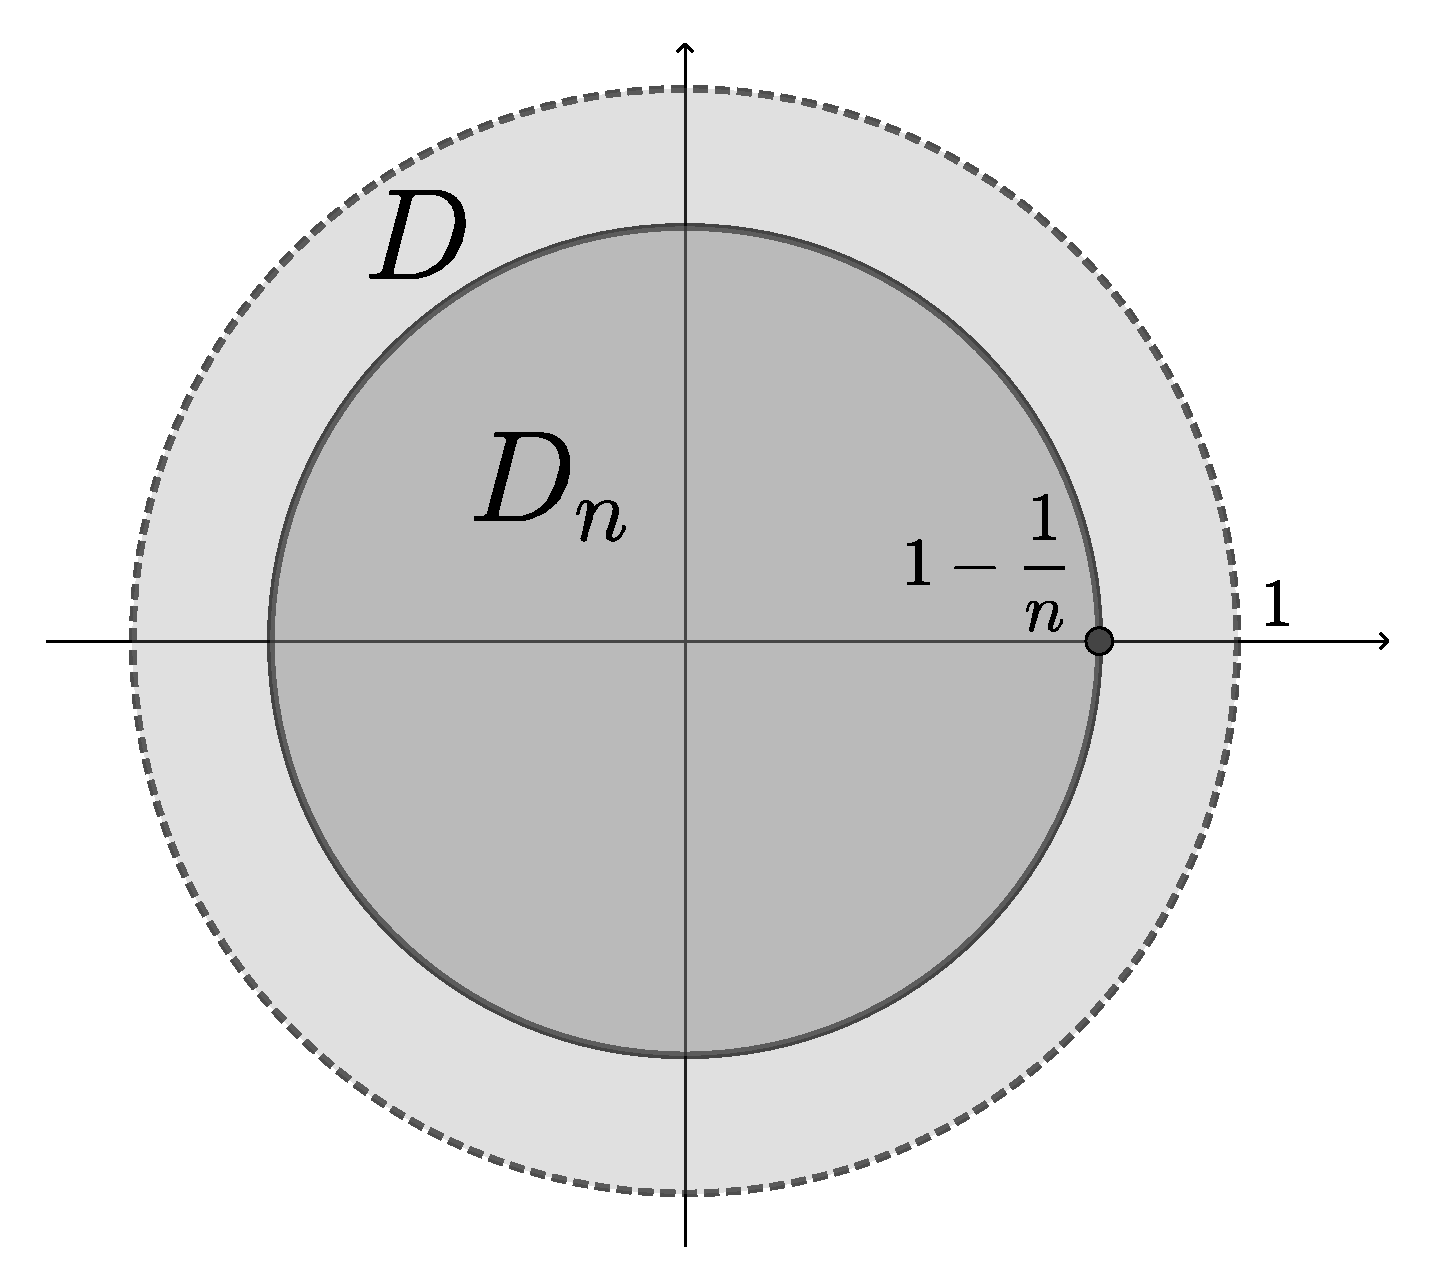
\includegraphics[height=4cm]{./pictures/no21.pdf}
       \caption{ $D_n=\Set{(x,y)  |  x^2+y^2 \leq  \left(1-\frac{1}{n}\right)^2 }$}\label{fig:no21}
     \end{figure}

     $(x,y) \in D$ に対して
     \[
       \frac{1-x}{\sqrt{1-x^2+y^2}} >0
     \]
     であるから,極限
     \[
       \lim_{n\to \infty} \iint_{D_n} \frac{1-x}{\sqrt{1-x^2-y^2}}\  dx dy
     \]
     が存在すれば広義積分は収束し,その極限値が求める広義積分の値である.極座標変換
     \[
       x=r\cos\theta, \quad y=r\sin \theta
     \]
     により,$r\theta$ 平面上の集合
     \[
       E_n =\Set{(r, \theta) | 0 \leq r \leq 1-\frac{1}{n}, \, 0 \leq \theta < 2\pi}
     \]
     が $xy$ 平面上の閉領域 $D_n$ に変換される.変換のヤコビアン
     は $J(r,\theta)=r$ であるから,$D_n$ 上の重積分は以下のように書き
     直せる.
     \begin{align*}
       \iint_{D_n} \frac{1-x}{\sqrt{1-x^2-y^2}}\ dx dy
       &= \iint_{E_n} \frac{1-r\cos\theta}{\sqrt{1-r^2}} |J(r,\theta)| \ dr d\theta\\
       &= \int_{0}^{2\pi}\left( \int_{0}^{1-\frac{1}{n}} \frac{r}{\sqrt{1-r^2}} \ dr 
         - \cos \theta \int_{0}^{1-\frac{1}{n}}\frac{r^2}{\sqrt{1-r^2}}\ dr\right) d\theta\\
       &= \left(\int_{0}^{2\pi} d\theta\right)\Big[\sqrt{1-r^2}\Big]_{0}^{1-\frac{1}{n}}
         -\left( \int_{0}^{2\pi}\cos\theta \ d\theta\right) \left( \int_{0}^{\frac{1}{n}}\frac{r^2}{\sqrt{1-r^2}} \ dr\right)\\
       &=2\pi\left(1-\sqrt{1-\left(1-\frac{1}{n}\right)^2}\right).
     \end{align*}
     よって,これより以下を得る.
     \[
       \iint_{D}\frac{1-x}{\sqrt{1-x^2-y^2}}\ dx dy
       = \lim_{n \to \infty} 2\pi \left(1-\sqrt{1-\left(1-\frac{1}{n}\right)^2}\right) = 2\pi.
     \]

   \item 集合 $D$ は有界ではないのでこれは広義積分である.自然数 $n$ に対して
     \[
       D_n = \Set{ (x,y)  |  -n \leq x \leq n, \, 0 \leq y \leq e^{-x^2} }
     \]
     とおくと,$\Set{D_n}$ は $D$ の増加近似列であり,これを図示すると
     図\ref{fig:no22}の通りである.
          \begin{figure}[h]
       \centering
       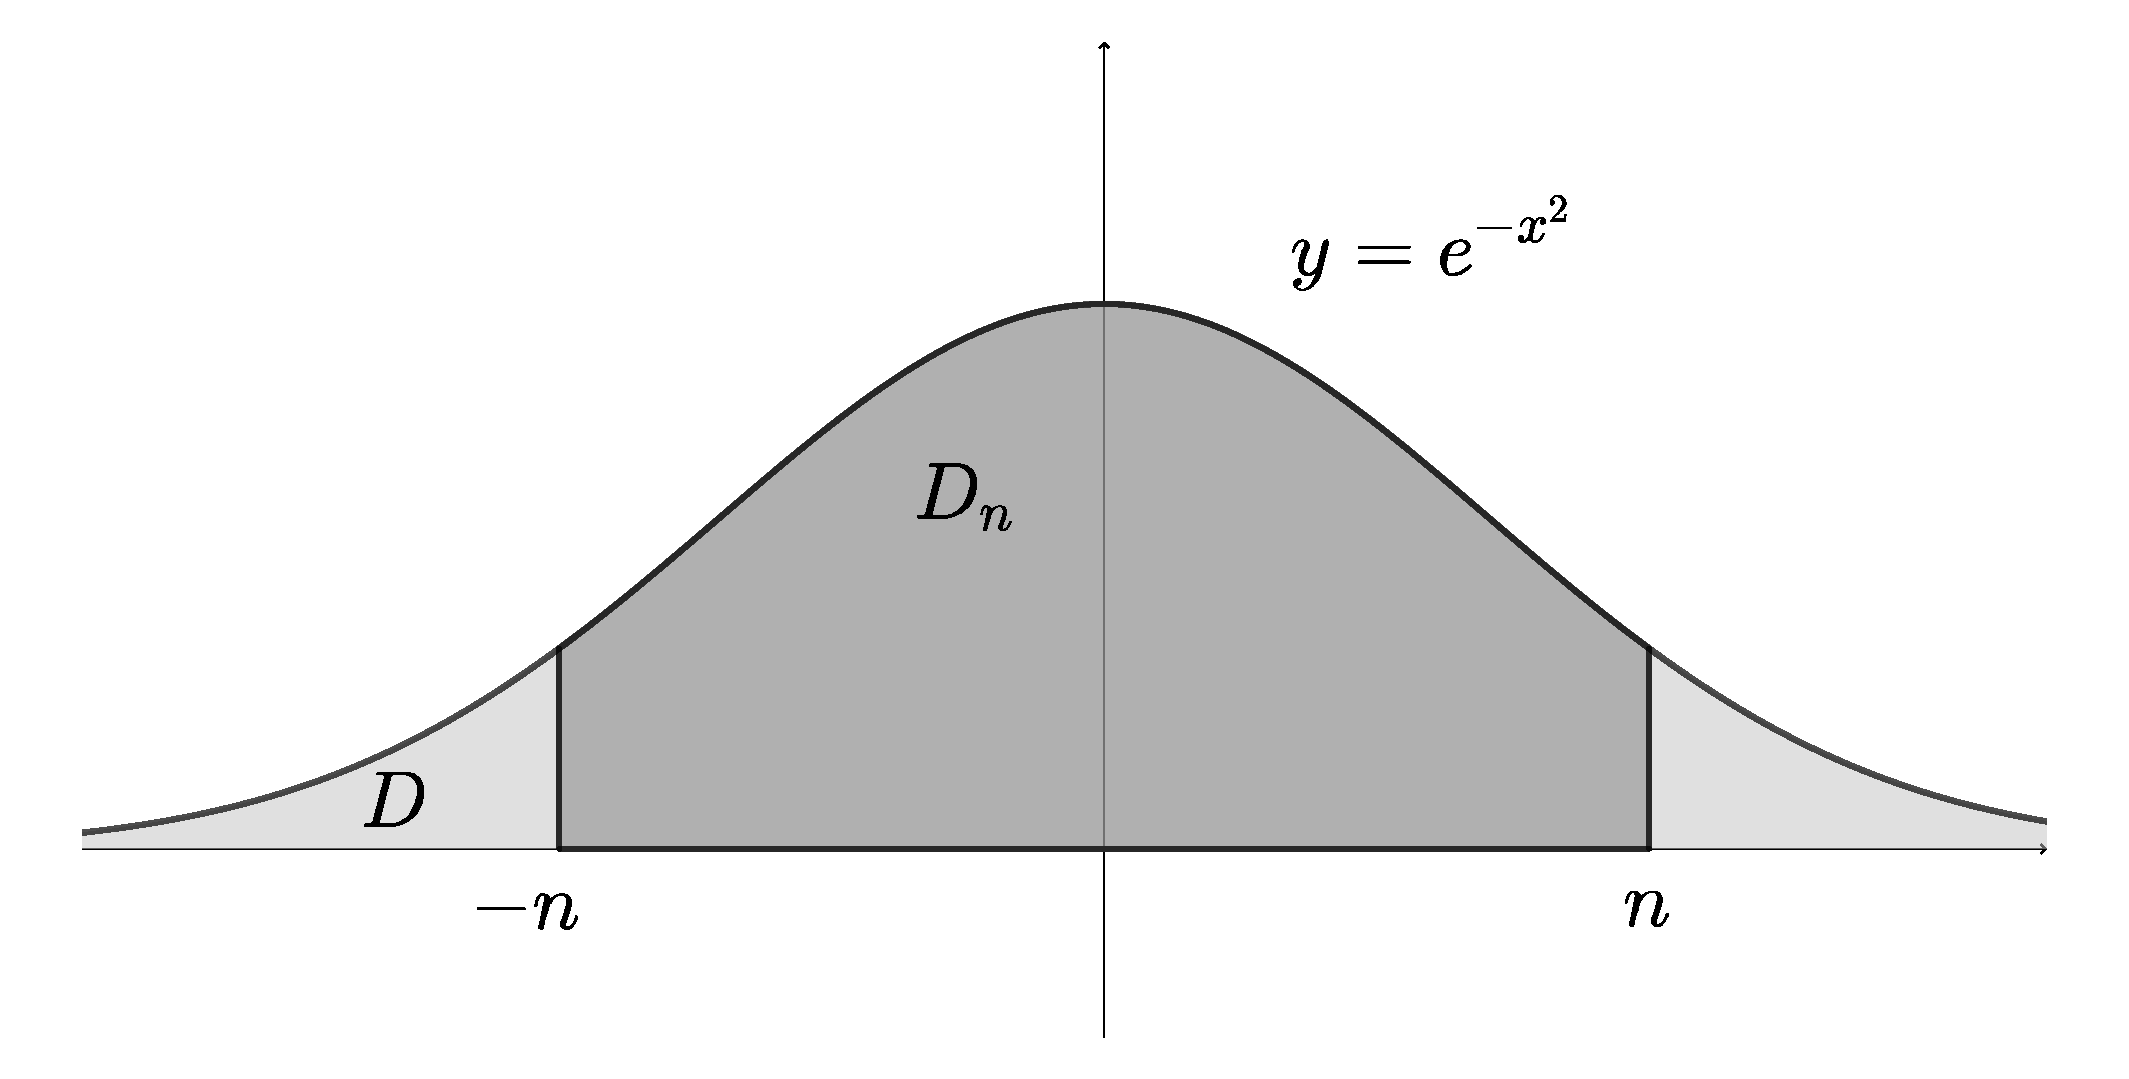
\includegraphics[height=4cm]{./pictures/no22.pdf}
       \caption{ $D_n=\Set{(x,y)  |  -n \leq x \leq n, \, 0 \leq y \leq e^{-x^2} }$}\label{fig:no22}
     \end{figure}
     $1 \geq0$ であるから,極限
     \[
       \lim_{n \to \infty} \iint_{D_n} dx dy
     \]
     が存在すれば広義積分は収束し,その極限値が求める広義積分の値である.
     各 $D_n$ は縦線集合と見なせるので $D_n$ 上の重積分は以下のように書き
     直せる.
     \[
       \iint_{D_n} dx dy = \int_{-n}^{n} \left( \int_{0}^{e^{-x^2}} dy \right) dx
       = \int_{-n}^{n} \Big[ y \Big]_{y=0}^{y=e^{-x^2}} dx 
       = \int_{-n}^{n} e^{-x^2} dx = 2 \int_{0}^{n} e^{-x^2} dx.
     \]
     従って,
     \[
       \iint_D dxdy = \lim_{n \to \infty} \iint_{D_n} dx dy = 2 \lim_{n \to \infty} \int_{0}^{n} e^{-x^2} dx
       = 2 \int_{0}^{\infty} e^{-x^2} \ dx 
     \]
     であるから上式最右辺に残った広義積分を求めればよい.
     \[
       I=\int_{0}^{\infty} e^{-x^2} \ dx, \quad I_n = \int_{0}^{n} e^{-x^2} \ dx
     \]
     とおくと,$\ds I=\lim_{n \to \infty} I_n$ である.また,自然
     数 $n$ に対して
     \[
       E_n =\Set{ (x,y) | 0 \leq x \leq n, \, 0 \leq y \leq n}
     \]
     とおくと,
     \[
       \left(I_n\right)^2 
       = \left( \int_{0}^{n} e^{-x^2} \ dx \right) \left( \int_{0}^{n} e^{-y^2} \ dy\right)
         = \int_{0}^{n} \left( \int_{0}^{n} e^{-x^2-y^2} dx \right) dy
         = \iint_{E_n} e^{-x^2-y^2} dx dy
     \]
     である.$\Set{ E_n}$ は第1象限
     \[
       E=\Set{(x,y) | 0 \leq x, \, 0 \leq y}
     \]
     の増加近似列であり,$e^{-x^2-y^2}>0$ だから $n \to \infty$ のと
     き $\left( I_n\right)^2$ が収束するなら
     \[
       I^2 = \left( \lim_{n \to \infty} I_n\right)^2 =\lim_{n \to \infty} \left( I_n\right)^2 
       = \lim_{n \to \infty} \iint_{E_n} e^{-x^2-y^2} dx dy
       = \iint_{E} e^{-x^2-y^2} dx dy
     \]
     である.従って,広義積分
     \[\tag{$\heartsuit$}
       \iint_{E} e^{-x^2-y^2} \ dx dy
     \]
     を求めればよい.自然数 $n$ に対して
     \[
       F_n = \Set{ (x,y) | x^2+y^2 \leq n^2, \, 0 \leq x, \, 0 \leq y}
     \]
     とすると,$\Set{F_n}$ は $E$ の増加近似列であり,$e^{-x^2-y^2}>0$ であるから極限
     \[
       \lim_{n \to \infty} \iint_{F_n} e^{-x^2-y^2} \ dx dy
     \]
     が存在すればその極限値が広義積分 $(\heartsuit)$ の値である.$E, E_n, F_n$ を図示すると,図\ref{fig:no22EF}の通りである.
     \begin{figure}[h]
       \centering
       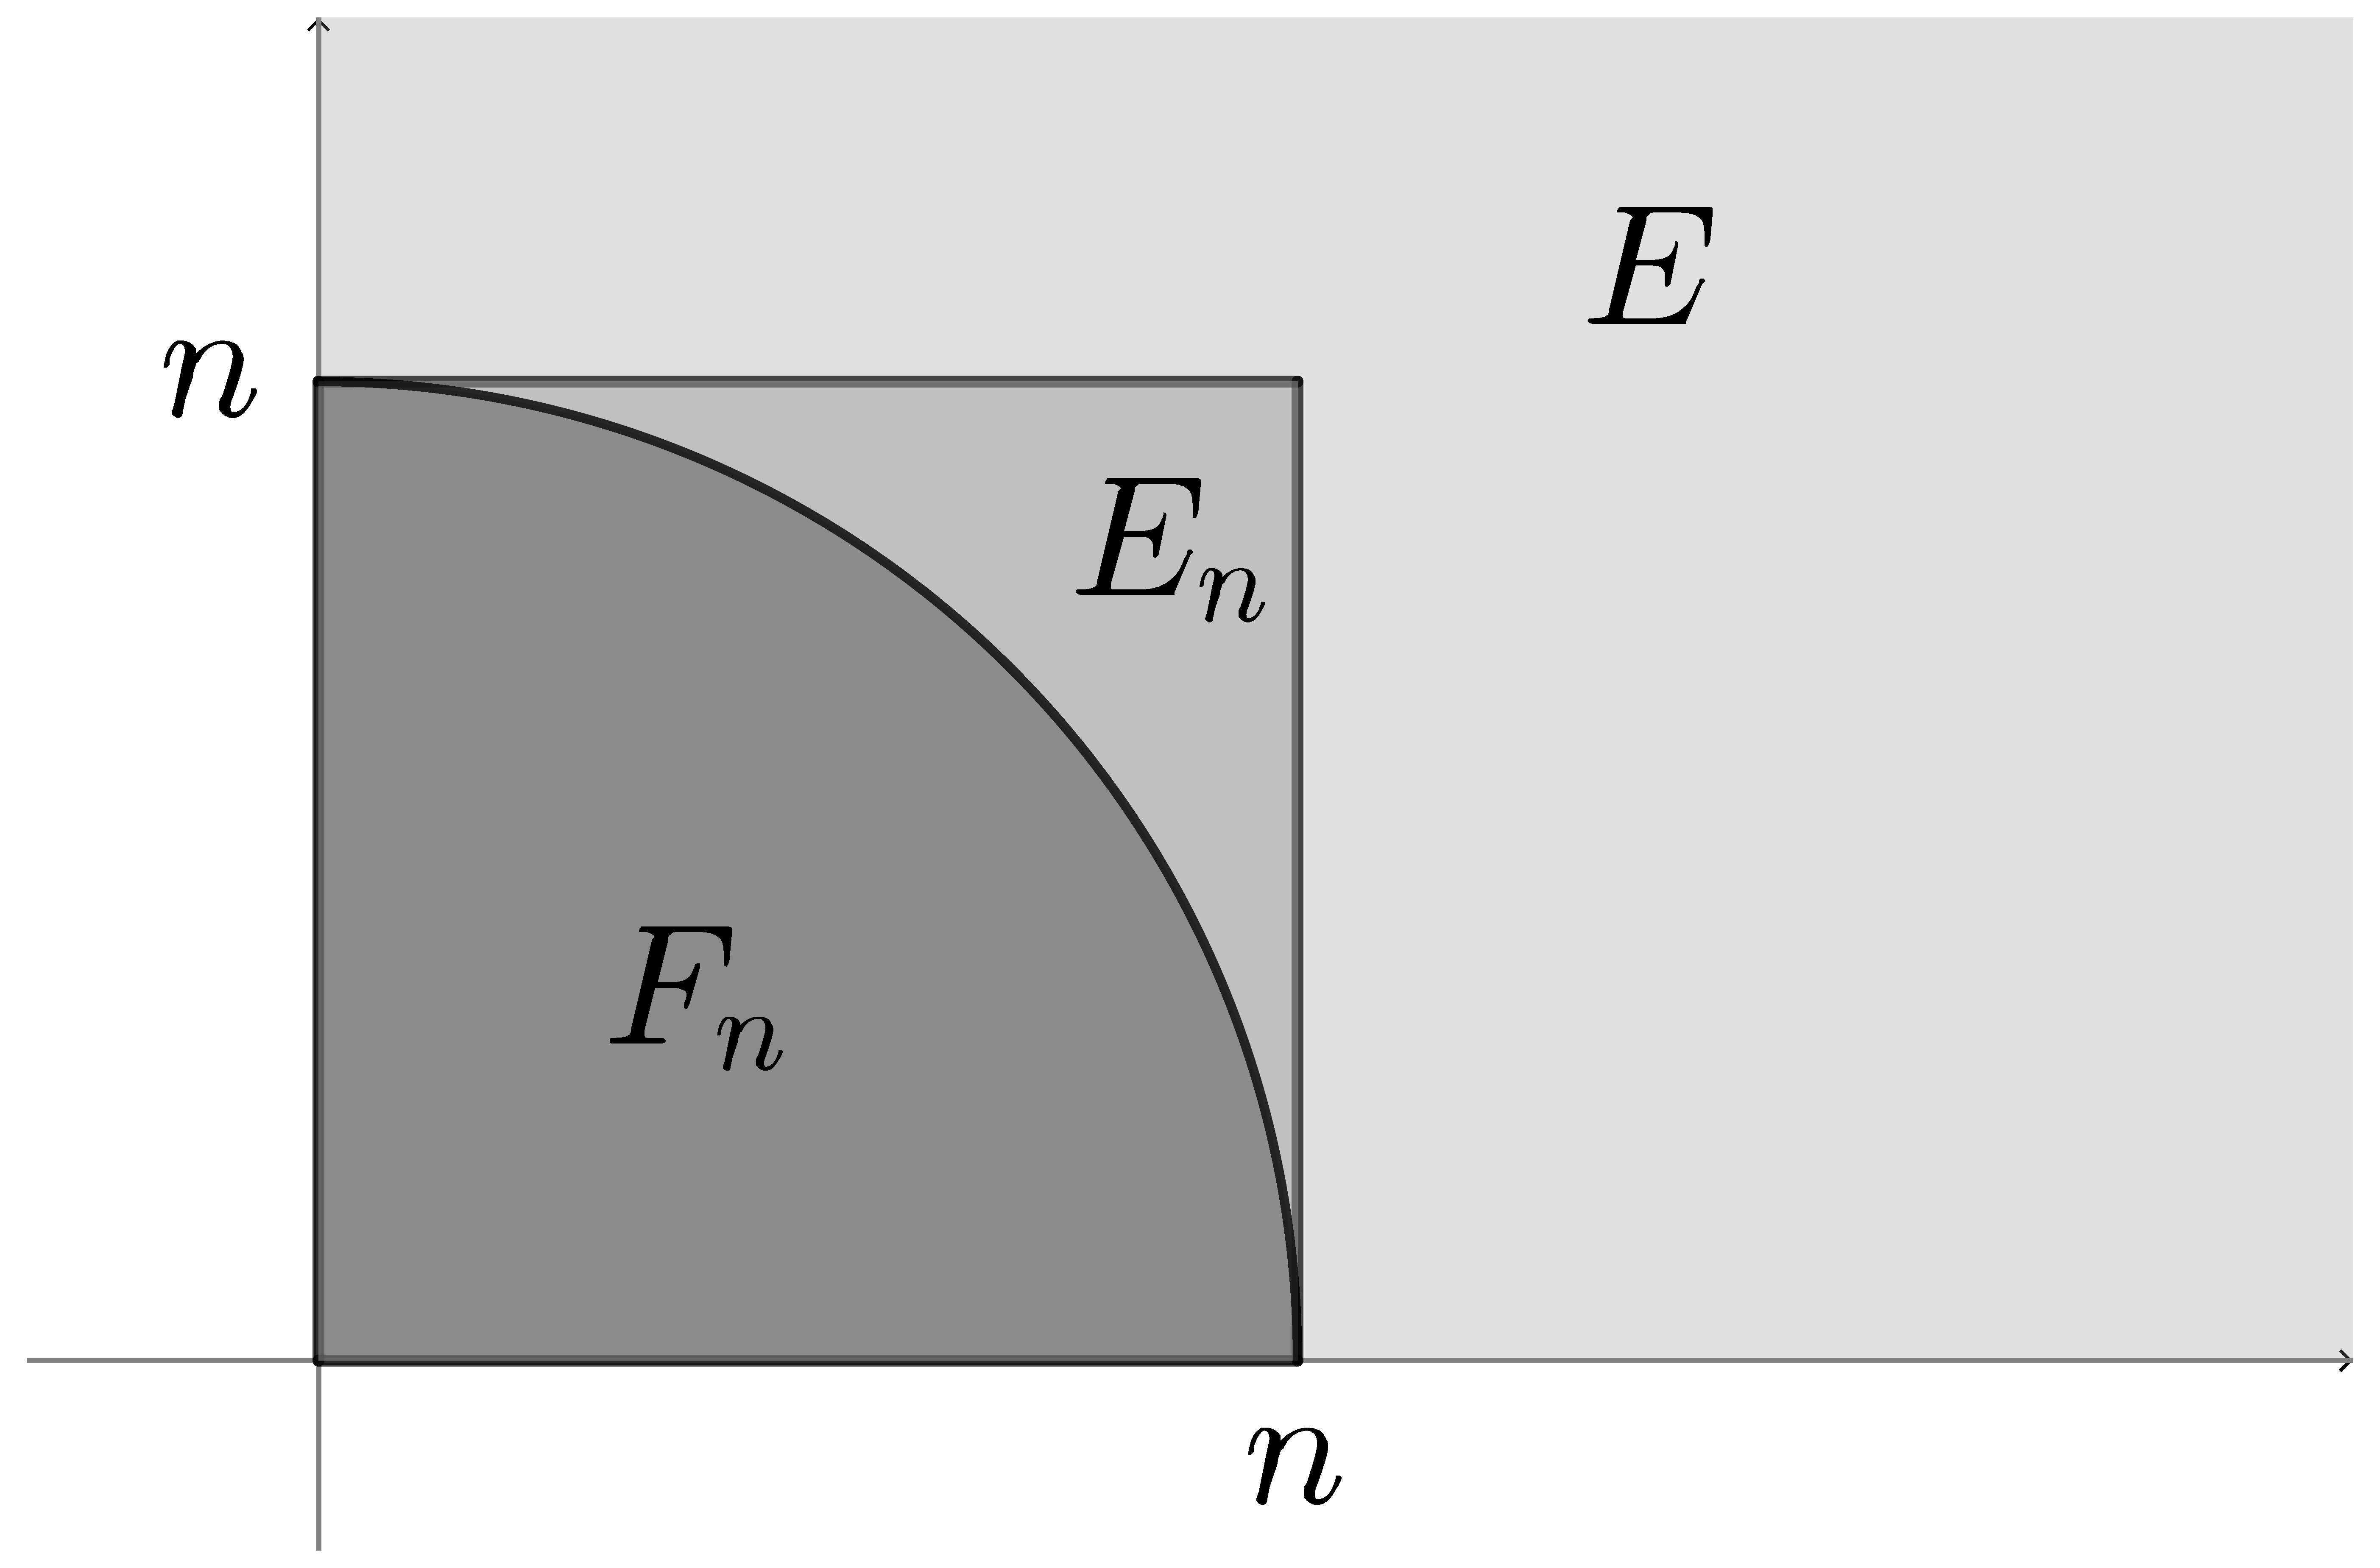
\includegraphics[height=4cm]{./pictures/no22EF.pdf}
       \caption{ $\Set{E_n}, \Set{F_n}$ はいずれも第1象限 $E$ の増加近似列である.}\label{fig:no22EF}
     \end{figure}


     極座標変換
     \[
       x=r\cos \theta, \quad y=r\sin \theta
     \]
     により,$r\theta$ 平面上の閉領域
     \[
       G_n =\Set{(r, \theta) | 0 \leq r \leq n, \, 0 \leq \theta \leq \frac{\pi}{2}}
     \]
     が $xy$ 平面上の閉領域 $F_n$ に変換される.変換のヤコビアン
     は $J(r, \theta)=r$ であるから,$F_n$ 上の重積分は以下のように書き
     直せる.
     \begin{align*}
       \iint_{F_n} e^{-x^2-y^2} dx dy 
       &= \iint_{G_n} e^{-r^2} |J(r,\theta)| \ dr d\theta 
         = \left( \int_{0}^{\frac{\pi}{2}} d\theta\right)\left(\int_{0}^{n}re^{-r^2} dr\right)\\
       & = \frac{\pi}{4}\left(1-e^{-n^2}\right).
     \end{align*}
     よって,
     \[
       \lim_{n \to \infty} \left(I_n\right)^2 = \iint_{E}e^{-x^2-y^2} dx dy 
       = \lim_{n \to \infty} \iint_{F_n} e^{-x^2-y^2} dx dy
       = \lim_{n \to \infty} \frac{\pi}{4}\left(1-e^{-n^2}\right) = \frac{\pi}{4}
     \]
     より $\left(I_n\right)^2$ は収束するので $\ds I^2 =
     \frac{\pi}{4}$ であり,明らかに $I>0$
     であるから,$\ds I=\frac{\sqrt{\pi}}{2}$ である.以上から,最終的な結論として以下を得る.
     \[
       \iint_{D} dx dy = 2 I = \sqrt{\pi}.
     \]

   \item 集合 $D$ は閉領域ではないので,これは広義積分である.自然
     数 $n$ に対して
     \[
       D_n = \Set{ (x,y)  |  \frac{1}{n} \leq x \leq 1, \, 0 \leq y \leq x }
     \]
     とすると,$\Set{D_n}$ は $D$ の増加近似列であり,図示すると図\ref{fig:no23}の通りである.
     \begin{figure}[h]
       \centering
       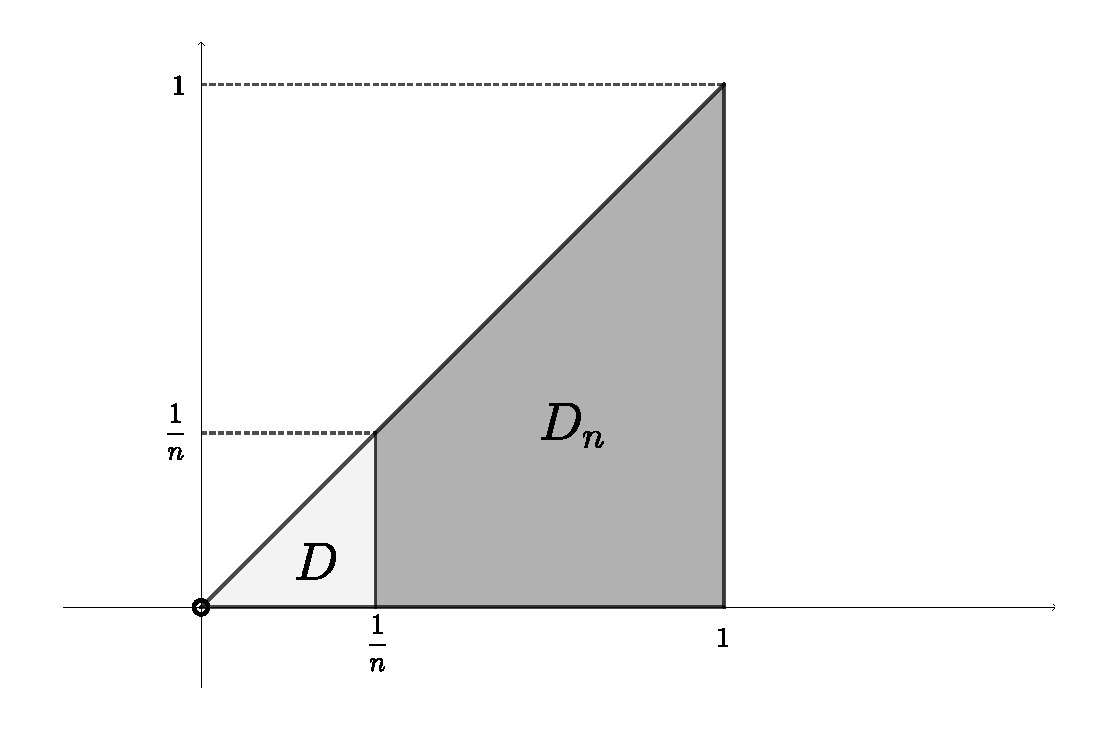
\includegraphics[height=4cm]{./pictures/no23.pdf}
       \caption{ $D_n=\Set{(x,y) |  \frac{1}{n} \leq x \leq 1, \, 0 \leq y \leq x }$}\label{fig:no23}
     \end{figure}
     
     $(x,y)\in D$ に対して $\sin \frac{y}{x} \geq 0$ であるから,極限
     \[
       \lim_{n \to \infty} \iint_{D_n} \sin \frac{y}{x} \ dx dy
     \]
     が存在すれば広義積分は収束し,その極限値が求める広義積分の値である.
     各 $D_n$ は縦線集合と見なせるので $D_n$ 上の重積分は以下のように書き
     直せる.
     \begin{align*}
       \iint_{D_n} \sin \frac{y}{x} \ dy dx
       &= \int_{\frac{1}{n}}^{1} \left( \int_{0}^{x} \sin \frac{y}{x} \ dy \right) dx
         =\int_{\frac{1}{n}}^{1} \left[-x \cos \frac{y}{x}\right]_{y=0}^{y=x} \ dx\\
       &= (1-\cos 1) \int_{\frac{1}{n}}^{1} x \ dx = \frac{1- \cos 1}{2} \left( 1- \frac{1}{n^2} \right).
     \end{align*}
     よって,これより以下を得る.
     \[
       \iint_D \sin \frac{y}{x} \ dx dy = \lim_{n \to \infty} \iint_{D_n} \sin \frac{y}{x} \ dx dy
       = \lim_{n \to \infty} \frac{1-\cos 1}{2} \left(1-\frac{1}{n^2}\right) = \frac{1-\cos 1}{2}.
     \]

   \item 集合 $\mathbb{R}^2$ は有界ではないので,これは広義積分である.
     被積分関数を $f(x,y)$ とおく.
     \[
       D_n=\Set{(x,y)  |  -n \leq x \leq n, \, -n \leq y \leq n }
     \]
     とすると $\Set{ D_n}$ は $\mathbb{R}^2$ の増加近似列である.任意
     の $(x,y) \in \mathbb{R}^2$ に対して $f(x,y)>0$ であるから,極限
     \[
       \lim_{n \to \infty} \iint_{D_n} f(x,y) \ dxdy
     \]
     が存在すれば広義積分は収束し,その極限値が求める広義積分の値であ
     る. $f(x,y)$ は $x, y, x+y$ の符号により以下のように分けられる.
     \[
       f(x,y)=
       \begin{cases}
         e^{-2(x+y)} & \left(0 \leq x , 0 \leq y \right)\\
         e^{-2y} & \left( x \leq 0 \leq y,  0 \leq x+y \right)\\
         e^{2x} & \left( x \leq 0 \leq y,  x+y \leq 0  \right)\\
         e^{2(x+y)} & \left( x \leq 0, y \leq 0 \right)\\
         e^{2y} & \left( y \leq 0 \leq x, x+y \leq 0\right)\\
         e^{-2x} & \left( y \leq 0 \leq x, 0 \leq x+y \right)
       \end{cases}
     \]
     そこで,図\ref{fig:no24}のように $D_n$ を以下の $6$ 個の閉領
     域 $D_n^1, \ldots, D_n^6$ に分割する.
     \begin{figure}[h]
       \centering
       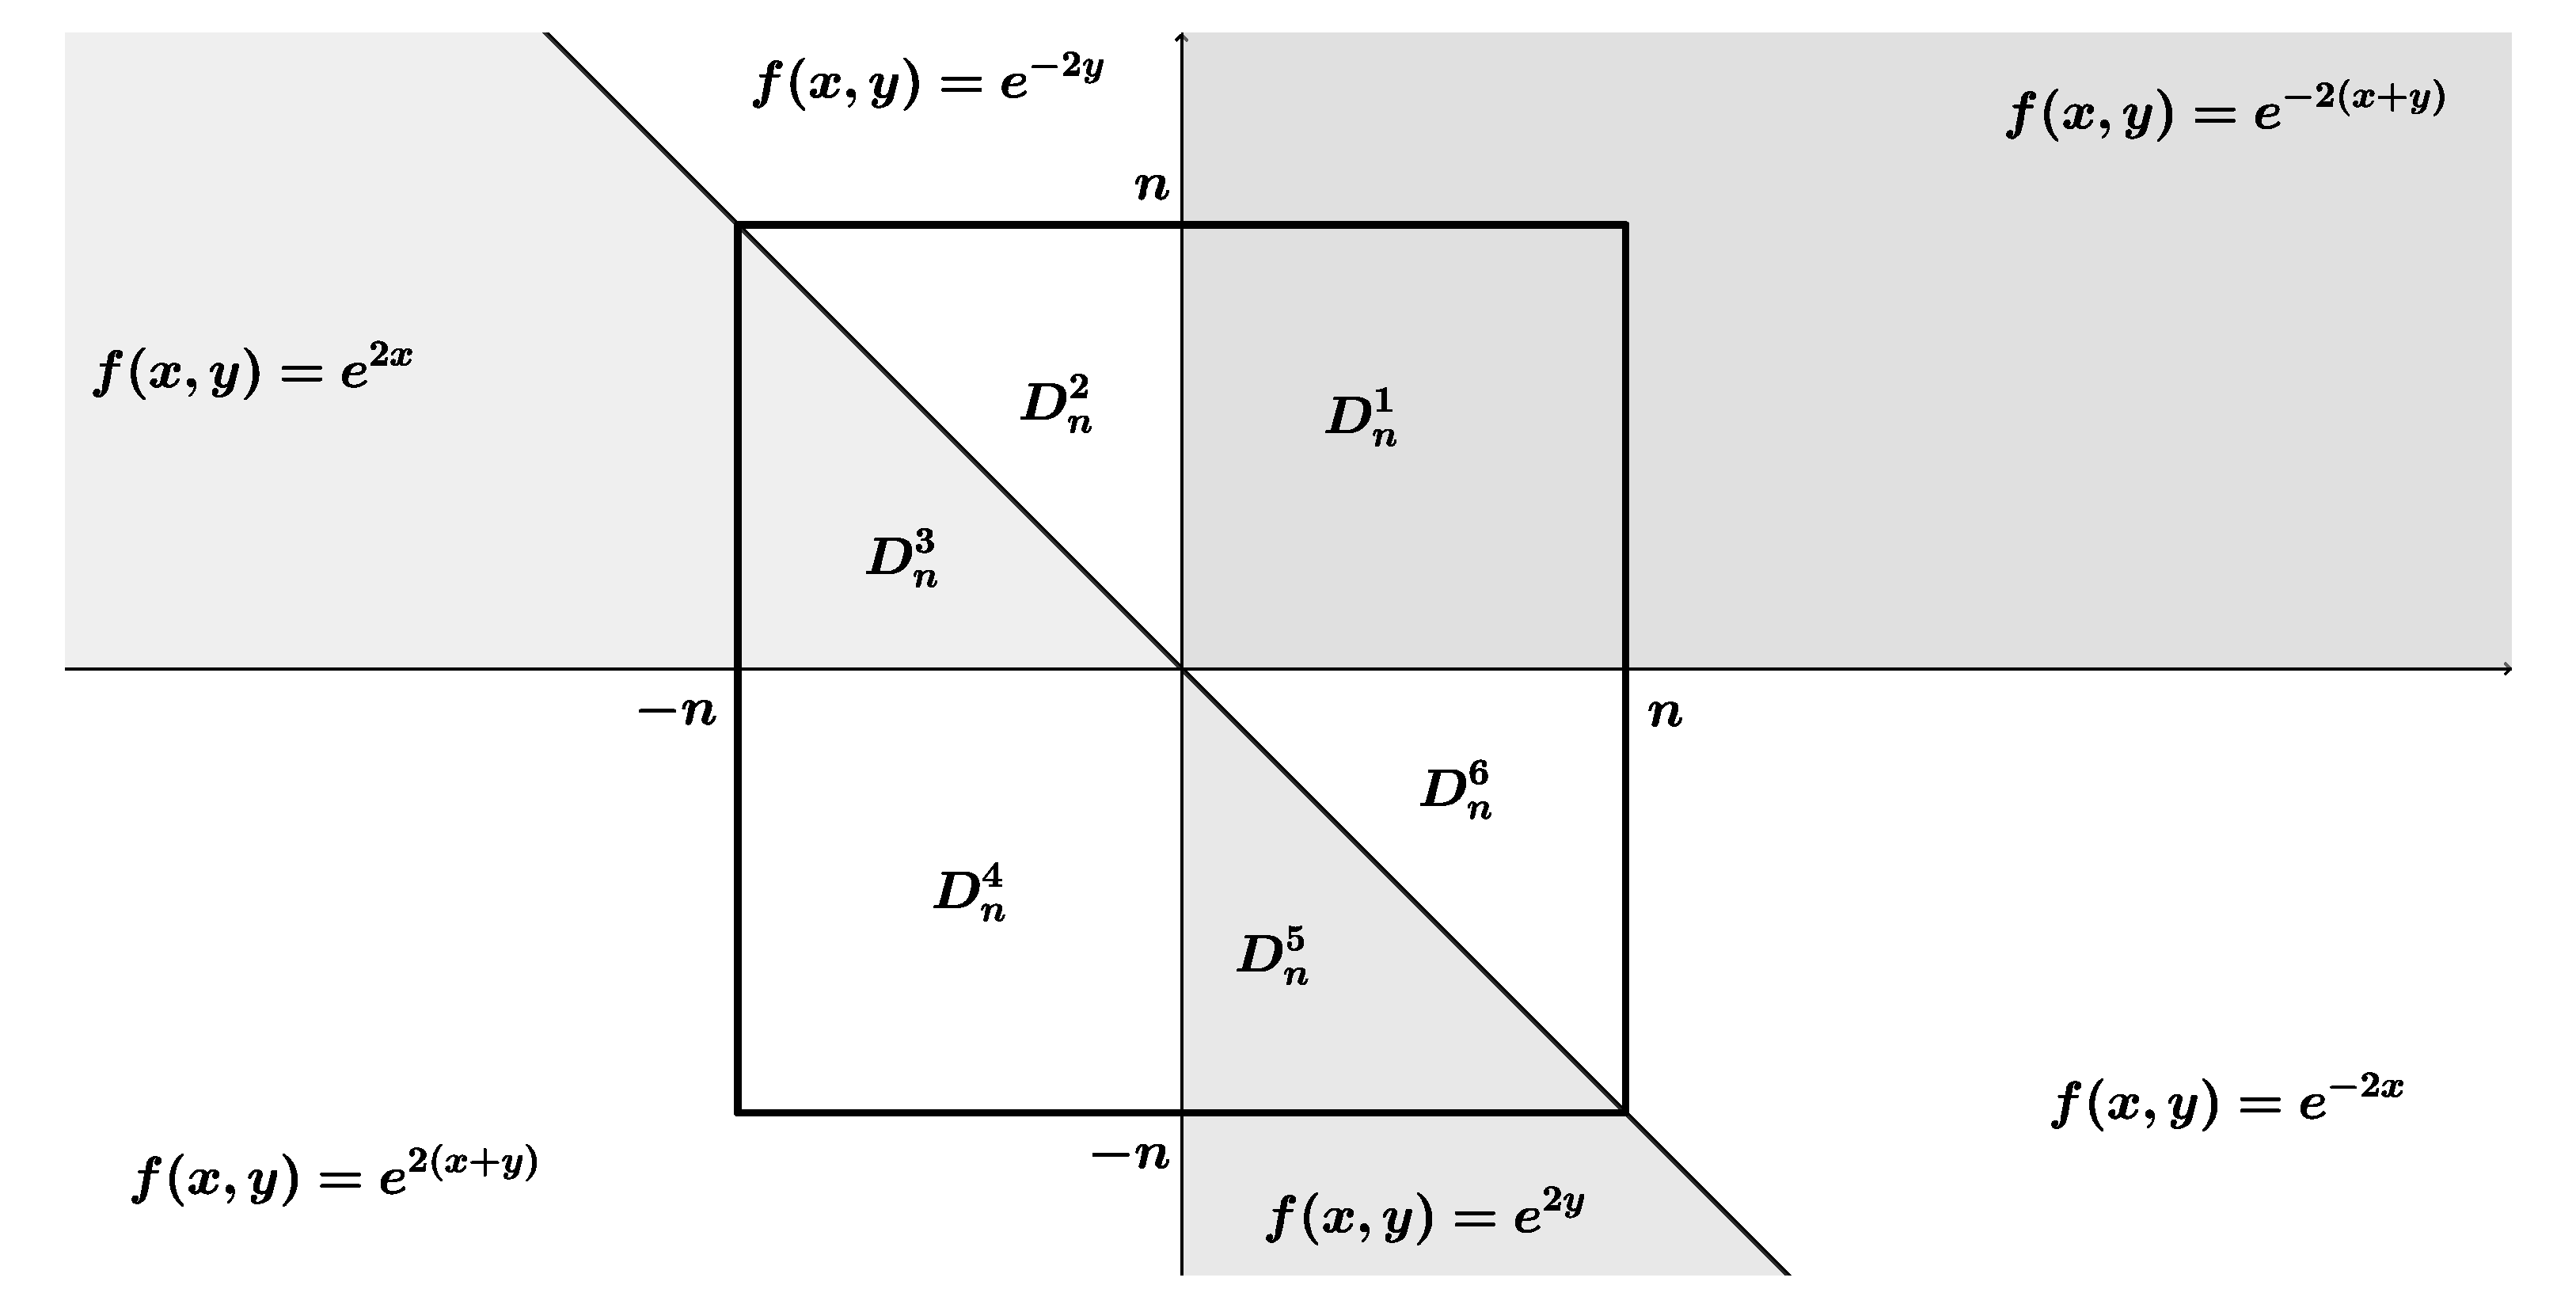
\includegraphics[height=5cm]{./pictures/no24.pdf}
       \caption{ $D_n= D_n^1 \cup D_n^2 \cup D_n^3 \cup D_n^4 \cup D_n^5 \cup D_n^6 $}\label{fig:no24}
     \end{figure}
     \begin{align*}
       & D_n^1 =\Set{(x,y)  |  0 \leq x \leq n, 0 \leq y \leq n}\\
       & D_n^2 =\Set{(x,y)  |  x \leq 0 \leq y, 0 \leq x+y, y \leq n} 
         = \Set{ (x,y) | 0 \leq y \leq n, \, -y \leq x \leq 0}\\
       & D_n^3 =\Set{(x,y)  | x \leq 0 \leq y, x+y \leq 0, -n \leq x}
         = \Set{(x,y) | -n \leq x \leq 0, \, 0 \leq y \leq -x}\\
       & D_n^4 =\Set{(x,y)  |  -n \leq x \leq 0, -n \leq y \leq 0 }\\
       & D_n^5 =\Set{(x,y)  |  y \leq 0 \leq x, x+y \leq 0, -n \leq y}
         =\Set{(x,y) | -n \leq y \leq 0, \, 0 \leq x \leq -y}\\
       & D_n^6 =\Set{(x,y)  |  y \leq 0 \leq x, 0 \leq x+y, x \leq n}
         =\Set{(x,y) | 0 \leq x \leq n, \, -x \leq y \leq 0}
     \end{align*}
     これらの共通部分はいずれも面積 $0$ の集合であるから
     \[
       \iint_{D_n} f(x,y)\ dxdy= \iint_{D_n^1}f(x,y)\ dxdy+\iint_{D_n^2}f(x,y)dxdy+ \cdots
       + \iint_{D_n^6} f(x,y)\ dxdy
     \]
     である.上式右辺の各重積分は次のように累次積分に書き直せる.
     \begin{align*}
       &\iint_{D_n^1} f(x,y) dx dy=\iint_{D_n^1} e^{-2(x+y)} dxdy
         = \int_{0}^{n} \int_{0}^{n} e^{-2(x+y)} dx dy
         = \frac{1-2e^{-2n}+e^{-4n}}{4},\\
       &\iint_{D_n^2} f(x,y) dxdy = \iint_{D_n^2} e^{-2y} dxdy
         = \int_{0}^{n} \int_{-y}^{0} e^{-2y} dx dy
         = \frac{1-2ne^{-2n}-e^{-2n}}{4},\\
       &\iint_{D_n^3} f(x,y) dxdy = \iint_{D_n^3} e^{2x} dxdy
         = \int_{-n}^{0} \int_{0}^{-x} e^{2x} dy dx
         = \frac{1-2ne^{-2n}-e^{-2n}}{4},\\
       &\iint_{D_n^4} f(x,y) dxdy= \iint_{D_n^4} e^{2(x+y)}dxdy
         =\int_{-n}^{0} \int_{-n}^{0} e^{2(x+y)} dxdy
         = \frac{1-2e^{-2n}+e^{-4n}}{4},\\
       &\iint_{D_n^5} f(x,y) dxdy= \iint_{D_n^5} e^{2y}dxdy
         = \int_{-n}^{0} \int_{0}^{-y} e^{2y} dx dy
         = \frac{1-2ne^{-2n}-e^{-2n}}{4},\\
       &\iint_{D_n^6} f(x,y) dxdy = \iint_{D_n^6} e^{-2x}dxdy
         =\int_{0}^{n} \int_{-x}^{0} e^{-2x}dydx
         = \frac{1-2ne^{-2n}-e^{-2n}}{4}.
     \end{align*}
     よって,これら6個の重積分を全て足し合わせて
     \[
       \iint_{D_n} f(x,y) \ dx dy = \frac{3}{2} - \frac{2}{e^{2n}} + \frac{1}{2e^{4n}} - \frac{2n}{e^{2n}}
     \]
     より,以下を得る.
     \[
       \iint_{D} e^{-|x|-|y|-|x+y|} \ dx dy
       = \lim_{n \to \infty} \left(  \frac{3}{2} - \frac{2}{e^{2n}} + \frac{1}{2e^{4n}} - \frac{2n}{e^{2n}}\right)
       = \frac{3}{2}.
     \]

   \end{enumerate}

\end{document}
